\documentclass{article}
% --- Korean translation support (xelatex + kotex) ---
\usepackage{kotex}
\usepackage{fontspec}
\setmainfont{NanumMyeongjo}[AutoFakeSlant=0.167]
\setsansfont{NanumGothic}[AutoFakeSlant=0.167]
\setmainhangulfont{NanumMyeongjo}[AutoFakeSlant=0.167]
\setsanshangulfont{NanumGothic}[AutoFakeSlant=0.167]
\setmonohangulfont{NanumGothicCoding}[AutoFakeSlant=0.167]
\setmonofont{NanumGothicCoding}[AutoFakeSlant=0.167]
\linespread{1.18}\selectfont
\renewcommand{\figurename}{그림}
\renewcommand{\tablename}{표}
\setlength{\parindent}{1.2em}
% --- end Korean support ---
\usepackage{amsmath}

\usepackage{arxiv}

% \usepackage[utf8]{inputenc} % allow utf-8 input % disabled for xelatex/kotex
% \usepackage[T1]{fontenc}    % use 8-bit T1 fonts % disabled for xelatex/kotex
\usepackage{hyperref}       % hyperlinks
\usepackage{url}            % simple URL typesetting
\usepackage{booktabs}       % professional-quality tables
\usepackage{amsfonts}       % blackboard math symbols
\usepackage{nicefrac}       % compact symbols for 1/2, etc.
\usepackage{microtype}      % microtypography
\usepackage{cleveref}       % smart cross-referencing
\usepackage{lipsum}         % Can be removed after putting your text content
\usepackage{graphicx}
\usepackage{doi}
\usepackage[numbers]{natbib}
\usepackage{multirow}
\usepackage{subcaption} % For creating subfigures




% Attempt to make hyperref and algorithmic work together better:
\newcommand{\theHalgorithm}{\arabic{algorithm}}

% Use the following line for the initial blind version submitted for review:

% If accepted, instead use the following line for the camera-ready submission:
% \usepackage[accepted]{icml2024}

% For theorems and such
\usepackage{amssymb}
\usepackage{mathtools}
\newcommand{\fix}{\marginpar{FIX}}
\newcommand{\new}{\marginpar{NEW}}
\RequirePackage{latexsym}
\RequirePackage{amsmath}
\RequirePackage{amsthm}
\RequirePackage{amssymb}
\RequirePackage{bm}
\RequirePackage{stmaryrd}
\RequirePackage{environ}
\RequirePackage{graphics}
\usepackage{dsfont}


\newcount\Comments  %
\Comments=1   %
\newcommand{\kibitz}[2]{\ifnum\Comments=1\textcolor{#1}{#2}\fi}
\usepackage{color}
\definecolor{red}{rgb}{1,0,0}
\newcommand{\owner}[1]{\kibitz{red}      {[CURRENT OWNER: #1]}}

\newcommand{\assign}[2][1]{\kibitz{red}      {[TODO(#1):#2]}}


\RequirePackage{xspace}
\newcommand{\Blackbox}{Black-box\xspace}
\newcommand{\blackbox}{black-box\xspace}


\makeatletter
\@ifpackageloaded{dsfont}{}{\newcommand{\mathds}[1]{\mathbb{#1}}}
\@ifpackageloaded{mathrsfs}{}{\newcommand{\mathscr}[1]{\mathcal{#1}}}
\makeatother

%%%%%%%% Environment %%%%%%%%%%%%%

% \begin{resize}[height]{width} \end{resize}
 \NewEnviron{resize}[2][!]{\resizebox{#2}{#1}{\BODY}} 
% \begin{rescale}[height_ratio]{width_ratio} \end{rescale}
 \NewEnviron{rescale}[2][]{\scalebox{#2}[#1]{\BODY}}

\makeatletter
\newcommand{\newreptheorem}[2]{
  \newtheorem*{rep@#1}{\rep@title} 
  \newenvironment{rep#1}[1]{\def\rep@title{#2 \ref*{##1}}\begin{rep@#1}}{\end{rep@#1}}
}
\makeatother
\newreptheorem{theorem}{Theorem}
\newreptheorem{claim}{Claim}

\usepackage{thm-restate}

%%%%%%%% Stock standard definitions %%%%%%%%%%%%%%%

% matrix with original font/boldsymbol/mathcal and tilde/bar/hat
\newcommand{\ab}{{\bm{a}}}
\newcommand{\bb}{{\bm{b}}}
\newcommand{\cbb}{{\bm{c}}}
\newcommand{\db}{{\bm{d}}}
\newcommand{\eb}{{\bm{e}}}
\newcommand{\fb}{{\bm{f}}}
\newcommand{\gb}{{\bm{g}}}
\newcommand{\hb}{{\bm{h}}}
\newcommand{\ib}{{\bm{i}}}
\newcommand{\jb}{{\bm{j}}}
\newcommand{\kb}{{\bm{k}}}
\newcommand{\lb}{{\bm{l}}}
\newcommand{\mb}{{\bm{m}}}
\newcommand{\nbb}{{\bm{n}}}
\newcommand{\ob}{{\bm{o}}}
\newcommand{\pb}{{\bm{p}}}
\newcommand{\qb}{{\bm{q}}}
\newcommand{\rb}{{\bm{r}}}
\newcommand{\sbb}{{\bm{s}}}
\newcommand{\tb}{{\bm{t}}}
\newcommand{\ub}{{\bm{u}}}
\newcommand{\vb}{{\bm{v}}}
\newcommand{\wb}{{\bm{w}}}
\newcommand{\xb}{{\bm{x}}}
\newcommand{\yb}{{\bm{y}}}
\newcommand{\zb}{{\bm{z}}}

\newcommand{\ba}{\ab}
\newcommand{\bc}{\cbb}
\newcommand{\bd}{\db}
\newcommand{\be}{\eb}
\newcommand{\bbf}{\fb}
\newcommand{\bff}{\fb}
\newcommand{\bg}{\gb}
\newcommand{\bh}{\hb}
\newcommand{\bi}{\ib}
\newcommand{\bj}{\jb}
\newcommand{\bk}{\kb}
\newcommand{\bl}{\lb}
\newcommand{\bbm}{\mb}
\newcommand{\bmm}{\mb}
\newcommand{\bn}{\nbb}
\newcommand{\bo}{\ob}
\newcommand{\bp}{\pb}
\newcommand{\bq}{\qb}
\newcommand{\br}{\rb}
\newcommand{\bs}{\sbb}
\newcommand{\bt}{\tb}
\newcommand{\bu}{\ub}
\newcommand{\bv}{\vb}
\newcommand{\bw}{\wb}
\newcommand{\bx}{\xb}
\newcommand{\by}{y^n}
\newcommand{\bz}{\zb}

% version with tilde
\newcommand{\atil}{\tilde{a}}
\newcommand{\btil}{\tilde{b}}
\newcommand{\ctil}{\tilde{c}}
\newcommand{\dtil}{\tilde{d}}
\newcommand{\etil}{\tilde{e}}
\newcommand{\ftil}{\tilde{f}}
\newcommand{\gtil}{\tilde{g}}
\newcommand{\htil}{\tilde{h}}
\newcommand{\itil}{\tilde{i}}
\newcommand{\jtil}{\tilde{j}}
\newcommand{\ktil}{\tilde{k}}
\newcommand{\ltil}{\tilde{l}}
\newcommand{\mtil}{\tilde{m}}
\newcommand{\ntil}{\tilde{n}}
\newcommand{\otil}{\tilde{o}}
\newcommand{\ptil}{\tilde{p}}
\newcommand{\qtil}{\tilde{q}}
\newcommand{\rtil}{\tilde{r}}
\newcommand{\stil}{\tilde{s}}
\newcommand{\ttil}{\tilde{t}}
\newcommand{\util}{\tilde{u}}
\newcommand{\vtil}{\tilde{v}}
\newcommand{\wtil}{\tilde{w}}
\newcommand{\xtil}{\tilde{x}}
\newcommand{\ytil}{\tilde{y}}
\newcommand{\ztil}{\tilde{z}}

\newcommand{\at}{\tilde{a}}
\newcommand{\bti}{\tilde{b}}
%\newcommand{\btt}{\tilde{b}}
\newcommand{\ct}{\tilde{c}}
\newcommand{\dt}{\tilde{d}}
\newcommand{\et}{\tilde{e}}
\newcommand{\ft}{\tilde{f}}
\newcommand{\gt}{\tilde{g}}
\newcommand{\hti}{\tilde{h}}
\newcommand{\htt}{\tilde{h}}
\newcommand{\iti}{\tilde{i}}
\newcommand{\itt}{\tilde{i}}
\newcommand{\jt}{\tilde{j}}
\newcommand{\kt}{\tilde{k}}
\newcommand{\lt}{\tilde{l}}
\newcommand{\mt}{\tilde{m}}
\newcommand{\nt}{\tilde{n}}
\newcommand{\ot}{\tilde{o}}
\newcommand{\pti}{\tilde{p}}
\newcommand{\ptt}{\tilde{p}}
\newcommand{\qt}{\tilde{q}}
\newcommand{\rt}{\tilde{r}}
\newcommand{\st}{\tilde{s}}
\newcommand{\tti}{\tilde{t}}
\newcommand{\ttt}{\tilde{t}}
\newcommand{\ut}{\tilde{u}}
\newcommand{\vti}{\tilde{v}}
\newcommand{\vtt}{\tilde{v}}
\newcommand{\wt}{\tilde{w}}
\newcommand{\xt}{\tilde{x}}
\newcommand{\yt}{\tilde{y}}
\newcommand{\zt}{\tilde{z}}

\newcommand{\abtil}{\tilde{\ab}}
\newcommand{\bbtil}{\tilde{\bb}}
\newcommand{\cbtil}{\tilde{\cbb}}
\newcommand{\dbtil}{\tilde{\db}}
\newcommand{\ebtil}{\tilde{\eb}}
\newcommand{\fbtil}{\tilde{\fb}}
\newcommand{\gbtil}{\tilde{\gb}}
\newcommand{\hbtil}{\tilde{\hb}}
\newcommand{\ibtil}{\tilde{\ib}}
\newcommand{\jbtil}{\tilde{\jb}}
\newcommand{\kbtil}{\tilde{\kb}}
\newcommand{\lbtil}{\tilde{\lb}}
\newcommand{\mbtil}{\tilde{\mb}}
\newcommand{\nbtil}{\tilde{\nbb}}
\newcommand{\obtil}{\tilde{\ob}}
\newcommand{\pbtil}{\tilde{\pb}}
\newcommand{\qbtil}{\tilde{\qb}}
\newcommand{\rbtil}{\tilde{\rb}}
\newcommand{\sbtil}{\tilde{\sbb}}
\newcommand{\tbtil}{\tilde{\tb}}
\newcommand{\ubtil}{\tilde{\ub}}
\newcommand{\vbtil}{\tilde{\vb}}
\newcommand{\wbtil}{\tilde{\wb}}
\newcommand{\xbtil}{\tilde{\xb}}
\newcommand{\ybtil}{\tilde{\yb}}
\newcommand{\zbtil}{\tilde{\zb}}

\newcommand{\batil}{\tilde{\ab}}
\newcommand{\bctil}{\tilde{\cbb}}
\newcommand{\bdtil}{\tilde{\db}}
\newcommand{\betil}{\tilde{\eb}}
\newcommand{\bftil}{\tilde{\fb}}
\newcommand{\bgtil}{\tilde{\gb}}
\newcommand{\bhtil}{\tilde{\hb}}
\newcommand{\bitil}{\tilde{\ib}}
\newcommand{\bjtil}{\tilde{\jb}}
\newcommand{\bktil}{\tilde{\kb}}
\newcommand{\bltil}{\tilde{\lb}}
\newcommand{\bmtil}{\tilde{\mb}}
\newcommand{\bntil}{\tilde{\nbb}}
\newcommand{\botil}{\tilde{\ob}}
\newcommand{\bptil}{\tilde{\pb}}
\newcommand{\bqtil}{\tilde{\qb}}
\newcommand{\brtil}{\tilde{\rb}}
\newcommand{\bstil}{\tilde{\sbb}}
\newcommand{\bttil}{\tilde{\tb}}
\newcommand{\butil}{\tilde{\ub}}
\newcommand{\bvtil}{\tilde{\vb}}
\newcommand{\bwtil}{\tilde{\wb}}
\newcommand{\bxtil}{\tilde{\xb}}
\newcommand{\bytil}{\tilde{\yb}}
\newcommand{\bztil}{\tilde{\zb}}

\newcommand{\bat}{\tilde{\ab}}
\newcommand{\bbt}{\tilde{\bb}}
\newcommand{\bct}{\tilde{\cbb}}
\newcommand{\bdt}{\tilde{\db}}
\newcommand{\bet}{\tilde{\eb}}
\newcommand{\bft}{\tilde{\fb}}
\newcommand{\bgt}{\tilde{\gb}}
\newcommand{\bht}{\tilde{\hb}}
\newcommand{\bit}{\tilde{\ib}}
\newcommand{\bjt}{\tilde{\jb}}
\newcommand{\bkt}{\tilde{\kb}}
\newcommand{\blt}{\tilde{\lb}}
\newcommand{\bmt}{\tilde{\mb}}
\newcommand{\bnt}{\tilde{\nbb}}
\newcommand{\boti}{\tilde{\ob}}
\newcommand{\boot}{\tilde{\ob}}
\newcommand{\bpt}{\tilde{\pb}}
\newcommand{\bqt}{\tilde{\qb}}
\newcommand{\brt}{\tilde{\rb}}
\newcommand{\bst}{\tilde{\sbb}}
\newcommand{\btti}{\tilde{\tb}}
\newcommand{\btt}{\tilde{\tb}}
\newcommand{\but}{\tilde{\ub}}
\newcommand{\bvt}{\tilde{\vb}}
\newcommand{\bwt}{\tilde{\wb}}
\newcommand{\bxt}{\tilde{\xb}}
\newcommand{\byt}{\tilde{\yb}}
\newcommand{\bzt}{\tilde{\zb}}

% version with hat
\newcommand{\ahat}{\hat{a}}
\newcommand{\bhat}{\hat{b}}
\newcommand{\chat}{\hat{c}}
\newcommand{\dhat}{\hat{d}}
\newcommand{\ehat}{\hat{e}}
\newcommand{\fhat}{\hat{f}}
\newcommand{\ghat}{\hat{g}}
\newcommand{\hhat}{\hat{h}}
\newcommand{\ihat}{\hat{i}}
\newcommand{\jhat}{\hat{j}}
\newcommand{\khat}{\hat{k}}
\newcommand{\lhat}{\hat{l}}
\newcommand{\mhat}{\hat{m}}
\newcommand{\nhat}{\hat{n}}
\newcommand{\ohat}{\hat{o}}
\newcommand{\phat}{\hat{p}}
\newcommand{\qhat}{\hat{q}}
\newcommand{\rhat}{\hat{r}}
\newcommand{\shat}{\hat{s}}
\newcommand{\that}{\hat{t}}
\newcommand{\uhat}{\hat{u}}
\newcommand{\vhat}{\hat{v}}
\newcommand{\what}{\hat{w}}
\newcommand{\xhat}{\hat{x}}
\newcommand{\yhat}{\hat{y}}
\newcommand{\zhat}{\hat{z}}
\newcommand{\pihat}{\hat{\pi}}

\newcommand{\abhat}{\hat{\ab}}
\newcommand{\bbhat}{\hat{\bb}}
\newcommand{\cbhat}{\hat{\cb}}
\newcommand{\dbhat}{\hat{\db}}
\newcommand{\ebhat}{\hat{\eb}}
\newcommand{\fbhat}{\hat{\fb}}
\newcommand{\gbhat}{\hat{\gb}}
\newcommand{\hbhat}{\hat{\hb}}
\newcommand{\ibhat}{\hat{\ib}}
\newcommand{\jbhat}{\hat{\jb}}
\newcommand{\kbhat}{\hat{\kb}}
\newcommand{\lbhat}{\hat{\lb}}
\newcommand{\mbhat}{\hat{\mb}}
\newcommand{\nbhat}{\hat{\nb}}
\newcommand{\obhat}{\hat{\ob}}
\newcommand{\pbhat}{\hat{\pb}}
\newcommand{\qbhat}{\hat{\qb}}
\newcommand{\rbhat}{\hat{\rb}}
\newcommand{\sbhat}{\hat{\sb}}
\newcommand{\tbhat}{\hat{\tb}}
\newcommand{\ubhat}{\hat{\ub}}
\newcommand{\vbhat}{\hat{\vb}}
\newcommand{\wbhat}{\hat{\wb}}
\newcommand{\xbhat}{\hat{\xb}}
\newcommand{\ybhat}{\hat{\yb}}
\newcommand{\zbhat}{\hat{\zb}}

\newcommand{\bahat}{\hat{\ab}}
\newcommand{\bchat}{\hat{\bc}}
\newcommand{\bdhat}{\hat{\db}}
\newcommand{\behat}{\hat{\eb}}
\newcommand{\bfhat}{\hat{\fb}}
\newcommand{\bghat}{\hat{\gb}}
\newcommand{\bhhat}{\hat{\hb}}
\newcommand{\bihat}{\hat{\ib}}
\newcommand{\bjhat}{\hat{\jb}}
\newcommand{\bkhat}{\hat{\kb}}
\newcommand{\blhat}{\hat{\lb}}
\newcommand{\bmhat}{\hat{\mb}}
\newcommand{\bnhat}{\hat{\nbb}}
\newcommand{\bohat}{\hat{\ob}}
\newcommand{\bphat}{\hat{\pb}}
\newcommand{\bqhat}{\hat{\qb}}
\newcommand{\brhat}{\hat{\rb}}
\newcommand{\bshat}{\hat{\sbb}}
\newcommand{\bthat}{\hat{\tb}}
\newcommand{\buhat}{\hat{\ub}}
\newcommand{\bvhat}{\hat{\vb}}
\newcommand{\bwhat}{\hat{\wb}}
\newcommand{\bxhat}{\hat{\xb}}
\newcommand{\byhat}{\hat{\yb}}
\newcommand{\bzhat}{\hat{\zb}}

% version with bar
\newcommand{\abar}{\bar{a}}
\newcommand{\bbar}{\bar{b}}
\newcommand{\cbar}{\bar{c}}
\newcommand{\dbar}{\bar{d}}
\newcommand{\ebar}{\bar{e}}
\newcommand{\fbar}{\bar{f}}
\newcommand{\gbar}{\bar{g}}
\newcommand{\hbr}{\bar{h}}
\newcommand{\ibar}{\bar{i}}
\newcommand{\jbar}{\bar{j}}
\newcommand{\kbar}{\bar{k}}
\newcommand{\lbar}{\bar{l}}
\newcommand{\mbar}{\bar{m}}
\newcommand{\nbar}{\bar{n}}
\newcommand{\obr}{\bar{o}}
\newcommand{\pbar}{\bar{p}}
\newcommand{\qbar}{\bar{q}}
\newcommand{\rbar}{\bar{r}}
\newcommand{\sbar}{\bar{s}}
\newcommand{\tbar}{\bar{t}}
\newcommand{\ubar}{\bar{u}}
\newcommand{\vbar}{\bar{v}}
\newcommand{\wbar}{\bar{w}}
\newcommand{\xbar}{\bar{x}}
\newcommand{\ybar}{\bar{y}}
\newcommand{\zbar}{\bar{z}}

\newcommand{\abbar}{\bar{\ab}}
\newcommand{\bbbar}{\bar{\bb}}
\newcommand{\cbbar}{\bar{\cb}}
\newcommand{\dbbar}{\bar{\db}}
\newcommand{\ebbar}{\bar{\eb}}
\newcommand{\fbbar}{\bar{\fb}}
\newcommand{\gbbar}{\bar{\gb}}
\newcommand{\hbbar}{\bar{\hb}}
\newcommand{\ibbar}{\bar{\ib}}
\newcommand{\jbbar}{\bar{\jb}}
\newcommand{\kbbar}{\bar{\kb}}
\newcommand{\lbbar}{\bar{\lb}}
\newcommand{\mbbar}{\bar{\mb}}
\newcommand{\nbbar}{\bar{\nbb}}
\newcommand{\obbar}{\bar{\ob}}
\newcommand{\pbbar}{\bar{\pb}}
\newcommand{\qbbar}{\bar{\qb}}
\newcommand{\rbbar}{\bar{\rb}}
\newcommand{\sbbar}{\bar{\sbb}}
\newcommand{\tbbar}{\bar{\tb}}
\newcommand{\ubbar}{\bar{\ub}}
\newcommand{\vbbar}{\bar{\vb}}
\newcommand{\wbbar}{\bar{\wb}}
\newcommand{\xbbar}{\bar{\xb}}
\newcommand{\ybbar}{\bar{\yb}}
\newcommand{\zbbar}{\bar{\zb}}

\newcommand{\babar}{\bar{\ab}}
\newcommand{\bcbar}{\bar{\bc}}
\newcommand{\bdbar}{\bar{\db}}
\newcommand{\bebar}{\bar{\eb}}
\newcommand{\bfbar}{\bar{\fb}}
\newcommand{\bgbar}{\bar{\gb}}
\newcommand{\bhbar}{\bar{\hb}}
\newcommand{\bibar}{\bar{\ib}}
\newcommand{\bjbar}{\bar{\jb}}
\newcommand{\bkbar}{\bar{\kb}}
\newcommand{\blbar}{\bar{\lb}}
\newcommand{\bmbar}{\bar{\mb}}
\newcommand{\bnbar}{\bar{\nbb}}
\newcommand{\bobar}{\bar{\ob}}
\newcommand{\bpbar}{\bar{\pb}}
\newcommand{\bqbar}{\bar{\qb}}
\newcommand{\brbar}{\bar{\rb}}
\newcommand{\bsbar}{\bar{\sbb}}
\newcommand{\btbar}{\bar{\tb}}
\newcommand{\bubar}{\bar{\ub}}
\newcommand{\bvbar}{\bar{\vb}}
\newcommand{\bwbar}{\bar{\wb}}
\newcommand{\bxbar}{\bar{\xb}}
\newcommand{\bybar}{\bar{\yb}}
\newcommand{\bzbar}{\bar{\zb}}

% matrix with original font/boldsymbol/mathcal and tilde/bar/hat
\newcommand{\Atil}{\tilde{A}}
\newcommand{\Btil}{\tilde{B}}
\newcommand{\Ctil}{\tilde{C}}
\newcommand{\Dtil}{\tilde{D}}
\newcommand{\Etil}{\tilde{E}}
\newcommand{\Ftil}{\tilde{F}}
\newcommand{\Gtil}{\tilde{G}}
\newcommand{\Htil}{\tilde{H}}
\newcommand{\Itil}{\tilde{I}}
\newcommand{\Jtil}{\tilde{J}}
\newcommand{\Ktil}{\tilde{K}}
\newcommand{\Ltil}{\tilde{L}}
\newcommand{\Mtil}{\tilde{M}}
\newcommand{\Ntil}{\tilde{N}}
\newcommand{\Otil}{\tilde{O}}
\newcommand{\Ptil}{\tilde{P}}
\newcommand{\Qtil}{\tilde{Q}}
\newcommand{\Rtil}{\tilde{R}}
\newcommand{\Stil}{\tilde{S}}
\newcommand{\Ttil}{\tilde{T}}
\newcommand{\Util}{\tilde{U}}
\newcommand{\Vtil}{\tilde{V}}
\newcommand{\Wtil}{\tilde{W}}
\newcommand{\Xtil}{\tilde{X}}
\newcommand{\Ytil}{\tilde{Y}}
\newcommand{\Ztil}{\tilde{Z}}

\newcommand{\At}{\tilde{A}}
\newcommand{\Bt}{\tilde{B}}
\newcommand{\Ct}{\tilde{C}}
\newcommand{\Dt}{\tilde{D}}
\newcommand{\Et}{\tilde{E}}
\newcommand{\Ft}{\tilde{F}}
\newcommand{\Gt}{\tilde{G}}
\newcommand{\Ht}{\tilde{H}}
\newcommand{\It}{\tilde{I}}
\newcommand{\Jt}{\tilde{J}}
\newcommand{\Kt}{\tilde{K}}
\newcommand{\Lt}{\tilde{L}}
\newcommand{\Mt}{\tilde{M}}
\newcommand{\Nt}{\tilde{N}}
\newcommand{\Ot}{\tilde{O}}
\newcommand{\Pt}{\tilde{P}}
\newcommand{\Qt}{\tilde{Q}}
\newcommand{\Rt}{\tilde{R}}
\newcommand{\St}{\tilde{S}}
\newcommand{\Tt}{\tilde{T}}
\newcommand{\Ut}{\tilde{U}}
\newcommand{\Vt}{\tilde{V}}
\newcommand{\Wt}{\tilde{W}}
\newcommand{\Xt}{\tilde{X}}
\newcommand{\Yt}{\tilde{Y}}
\newcommand{\Zt}{\tilde{Z}}

\newcommand{\Atilde}{\widetilde{A}}
\newcommand{\Btilde}{\widetilde{B}}
\newcommand{\Ctilde}{\widetilde{C}}
\newcommand{\Dtilde}{\widetilde{D}}
\newcommand{\Etilde}{\widetilde{E}}
\newcommand{\Ftilde}{\widetilde{F}}
\newcommand{\Gtilde}{\widetilde{G}}
\newcommand{\Htilde}{\widetilde{H}}
\newcommand{\Itilde}{\widetilde{I}}
\newcommand{\Jtilde}{\widetilde{J}}
\newcommand{\Ktilde}{\widetilde{K}}
\newcommand{\Ltilde}{\widetilde{L}}
\newcommand{\Mtilde}{\widetilde{M}}
\newcommand{\Ntilde}{\widetilde{N}}
\newcommand{\Otilde}{\widetilde{O}}
\newcommand{\Ptilde}{\widetilde{P}}
\newcommand{\Qtilde}{\widetilde{Q}}
\newcommand{\Rtilde}{\widetilde{R}}
\newcommand{\Stilde}{\widetilde{S}}
\newcommand{\Ttilde}{\widetilde{T}}
\newcommand{\Utilde}{\widetilde{U}}
\newcommand{\Vtilde}{\widetilde{V}}
\newcommand{\Wtilde}{\widetilde{W}}
\newcommand{\Xtilde}{\widetilde{X}}
\newcommand{\Ytilde}{\widetilde{Y}}
\newcommand{\Ztilde}{\widetilde{Z}}

\newcommand{\Abar}{\bar{A}}
\newcommand{\Bbar}{\bar{B}}
\newcommand{\Cbar}{\bar{C}}
\newcommand{\Dbar}{\bar{D}}
\newcommand{\Ebar}{\bar{E}}
\newcommand{\Fbar}{\bar{F}}
\newcommand{\Gbar}{\bar{G}}
\newcommand{\Hbar}{\bar{H}}
\newcommand{\Ibar}{\bar{I}}
\newcommand{\Jbar}{\bar{J}}
\newcommand{\Kbar}{\bar{K}}
\newcommand{\Lbar}{\bar{L}}
\newcommand{\Mbar}{\bar{M}}
\newcommand{\Nbar}{\bar{N}}
\newcommand{\Obar}{\bar{O}}
\newcommand{\Pbar}{\bar{P}}
\newcommand{\Qbar}{\bar{Q}}
\newcommand{\Rbar}{\bar{R}}
\newcommand{\Sbar}{\bar{S}}
\newcommand{\Tbar}{\bar{T}}
\newcommand{\Ubar}{\bar{U}}
\newcommand{\Vbar}{\bar{V}}
\newcommand{\Wbar}{\bar{W}}
\newcommand{\Xbar}{\bar{X}}
\newcommand{\Ybar}{\bar{Y}}
\newcommand{\Zbar}{\bar{Z}}

\newcommand{\Ahat}{\hat{A}}
\newcommand{\Bhat}{\hat{B}}
\newcommand{\Chat}{\hat{C}}
\newcommand{\Dhat}{\hat{D}}
\newcommand{\Ehat}{\hat{E}}
\newcommand{\Fhat}{\hat{F}}
\newcommand{\Ghat}{\hat{G}}
\newcommand{\Hhat}{\hat{H}}
\newcommand{\Ihat}{\hat{I}}
\newcommand{\Jhat}{\hat{J}}
\newcommand{\Khat}{\hat{K}}
\newcommand{\Lhat}{\hat{L}}
\newcommand{\Mhat}{\hat{M}}
\newcommand{\Nhat}{\hat{N}}
\newcommand{\Ohat}{\hat{O}}
\newcommand{\Phat}{\hat{P}}
\newcommand{\Qhat}{\hat{Q}}
\newcommand{\Rhat}{\hat{R}}
\newcommand{\Shat}{\hat{S}}
\newcommand{\That}{\hat{T}}
\newcommand{\Uhat}{\hat{U}}
\newcommand{\Vhat}{\hat{V}}
\newcommand{\What}{\hat{W}}
\newcommand{\Xhat}{\hat{X}}
\newcommand{\Yhat}{\hat{Y}}
\newcommand{\Zhat}{\hat{Z}}

\newcommand{\Ab}{\bm{{A}}}
\newcommand{\Bb}{\bm{{B}}}
\newcommand{\Cb}{\bm{{C}}}
\newcommand{\Db}{\bm{{D}}}
\newcommand{\Eb}{\bm{{E}}}
\newcommand{\Fb}{\bm{{F}}}
\newcommand{\Gb}{\bm{{G}}}
\newcommand{\Hb}{\bm{{H}}}
\newcommand{\Ib}{\bm{{I}}}
\newcommand{\Jb}{\bm{{J}}}
\newcommand{\Kb}{\bm{{K}}}
\newcommand{\Lb}{\bm{{L}}}
\newcommand{\Mb}{\bm{{M}}}
\newcommand{\Nb}{\bm{{N}}}
\newcommand{\Ob}{\bm{{O}}}
\newcommand{\Pb}{\bm{{P}}}
\newcommand{\Qb}{\bm{{Q}}}
\newcommand{\Rb}{\bm{{R}}}
\newcommand{\Sbb}{\bm{{S}}}
\newcommand{\Tb}{\bm{{T}}}
\newcommand{\Ub}{\bm{{U}}}
\newcommand{\Vb}{\bm{{V}}}
\newcommand{\Wb}{\bm{{W}}}
\newcommand{\Xb}{\bm{{X}}}
\newcommand{\Yb}{\bm{{Y}}}
\newcommand{\Zb}{\bm{{Z}}}

\newcommand{\bA}{\bm{{A}}}
\newcommand{\bB}{\bm{{B}}}
\newcommand{\bC}{\bm{{C}}}
\newcommand{\bD}{\bm{{D}}}
\newcommand{\bE}{\bm{{E}}}
\newcommand{\bF}{\bm{{F}}}
\newcommand{\bG}{\bm{{G}}}
\newcommand{\bH}{\bm{{H}}}
\newcommand{\bI}{\bm{{I}}}
\newcommand{\bJ}{\bm{{J}}}
\newcommand{\bK}{\bm{{K}}}
\newcommand{\bL}{\bm{{L}}}
\newcommand{\bM}{\bm{{M}}}
\newcommand{\bN}{\bm{{N}}}
\newcommand{\bO}{\bm{{O}}}
\newcommand{\bP}{\bm{{P}}}
\newcommand{\bQ}{\bm{{Q}}}
\newcommand{\bR}{\bm{{R}}}
\newcommand{\bS}{\bm{{S}}}
\newcommand{\bT}{\bm{{T}}}
\newcommand{\bU}{\bm{{U}}}
\newcommand{\bV}{\bm{{V}}}
\newcommand{\bW}{\bm{{W}}}
\newcommand{\bX}{\bm{{X}}}
\newcommand{\bY}{\bm{{Y}}}
\newcommand{\bZ}{\bm{{Z}}}

\newcommand{\Abtil}{\tilde{\Ab}}
\newcommand{\Bbtil}{\tilde{\Bb}}
\newcommand{\Cbtil}{\tilde{\Cb}}
\newcommand{\Dbtil}{\tilde{\Db}}
\newcommand{\Ebtil}{\tilde{\Eb}}
\newcommand{\Fbtil}{\tilde{\Fb}}
\newcommand{\Gbtil}{\tilde{\Gb}}
\newcommand{\Hbtil}{\tilde{\Hb}}
\newcommand{\Ibtil}{\tilde{\Ib}}
\newcommand{\Jbtil}{\tilde{\Jb}}
\newcommand{\Kbtil}{\tilde{\Kb}}
\newcommand{\Lbtil}{\tilde{\Lb}}
\newcommand{\Mbtil}{\tilde{\Mb}}
\newcommand{\Nbtil}{\tilde{\Nb}}
\newcommand{\Obtil}{\tilde{\Ob}}
\newcommand{\Pbtil}{\tilde{\Pb}}
\newcommand{\Qbtil}{\tilde{\Qb}}
\newcommand{\Rbtil}{\tilde{\Rb}}
\newcommand{\Sbtil}{\tilde{\Sbb}}
\newcommand{\Tbtil}{\tilde{\Tb}}
\newcommand{\Ubtil}{\tilde{\Ub}}
\newcommand{\Vbtil}{\tilde{\Vb}}
\newcommand{\Wbtil}{\tilde{\Wb}}
\newcommand{\Xbtil}{\tilde{\Xb}}
\newcommand{\Ybtil}{\tilde{\Yb}}
\newcommand{\Zbtil}{\tilde{\Zb}}

\newcommand{\bAt}{\tilde{\Ab}}
\newcommand{\bBt}{\tilde{\Bb}}
\newcommand{\bCt}{\tilde{\Cb}}
\newcommand{\bDt}{\tilde{\Db}}
\newcommand{\bEt}{\tilde{\Eb}}
\newcommand{\bFt}{\tilde{\Fb}}
\newcommand{\bGt}{\tilde{\Gb}}
\newcommand{\bHt}{\tilde{\Hb}}
\newcommand{\bIt}{\tilde{\Ib}}
\newcommand{\bJt}{\tilde{\Jb}}
\newcommand{\bKt}{\tilde{\Kb}}
\newcommand{\bLt}{\tilde{\Lb}}
\newcommand{\bMt}{\tilde{\Mb}}
\newcommand{\bNt}{\tilde{\Nb}}
\newcommand{\bOt}{\tilde{\Ob}}
\newcommand{\bPt}{\tilde{\Pb}}
\newcommand{\bQt}{\tilde{\Qb}}
\newcommand{\bRt}{\tilde{\Rb}}
\newcommand{\bSt}{\tilde{\Sbb}}
\newcommand{\bTt}{\tilde{\Tb}}
\newcommand{\bUt}{\tilde{\Ub}}
\newcommand{\bVt}{\tilde{\Vb}}
\newcommand{\bWt}{\tilde{\Wb}}
\newcommand{\bXt}{\tilde{\Xb}}
\newcommand{\bYt}{\tilde{\Yb}}
\newcommand{\bZt}{\tilde{\Zb}}

\newcommand{\bAtil}{\tilde{\Ab}}
\newcommand{\bBtil}{\tilde{\Bb}}
\newcommand{\bCtil}{\tilde{\Cb}}
\newcommand{\bDtil}{\tilde{\Db}}
\newcommand{\bEtil}{\tilde{\Eb}}
\newcommand{\bFtil}{\tilde{\Fb}}
\newcommand{\bGtil}{\tilde{\Gb}}
\newcommand{\bHtil}{\tilde{\Hb}}
\newcommand{\bItil}{\tilde{\Ib}}
\newcommand{\bJtil}{\tilde{\Jb}}
\newcommand{\bKtil}{\tilde{\Kb}}
\newcommand{\bLtil}{\tilde{\Lb}}
\newcommand{\bMtil}{\tilde{\Mb}}
\newcommand{\bNtil}{\tilde{\Nb}}
\newcommand{\bOtil}{\tilde{\Ob}}
\newcommand{\bPtil}{\tilde{\Pb}}
\newcommand{\bQtil}{\tilde{\Qb}}
\newcommand{\bRtil}{\tilde{\Rb}}
\newcommand{\bStil}{\tilde{\Sbb}}
\newcommand{\bTtil}{\tilde{\Tb}}
\newcommand{\bUtil}{\tilde{\Ub}}
\newcommand{\bVtil}{\tilde{\Vb}}
\newcommand{\bWtil}{\tilde{\Wb}}
\newcommand{\bXtil}{\tilde{\Xb}}
\newcommand{\bYtil}{\tilde{\Yb}}
\newcommand{\bZtil}{\tilde{\Zb}}

\newcommand{\bAtilde}{\widetilde{\Ab}}
\newcommand{\bBtilde}{\widetilde{\Bb}}
\newcommand{\bCtilde}{\widetilde{\Cb}}
\newcommand{\bDtilde}{\widetilde{\Db}}
\newcommand{\bEtilde}{\widetilde{\Eb}}
\newcommand{\bFtilde}{\widetilde{\Fb}}
\newcommand{\bGtilde}{\widetilde{\Gb}}
\newcommand{\bHtilde}{\widetilde{\Hb}}
\newcommand{\bItilde}{\widetilde{\Ib}}
\newcommand{\bJtilde}{\widetilde{\Jb}}
\newcommand{\bKtilde}{\widetilde{\Kb}}
\newcommand{\bLtilde}{\widetilde{\Lb}}
\newcommand{\bMtilde}{\widetilde{\Mb}}
\newcommand{\bNtilde}{\widetilde{\Nb}}
\newcommand{\bOtilde}{\widetilde{\Ob}}
\newcommand{\bPtilde}{\widetilde{\Pb}}
\newcommand{\bQtilde}{\widetilde{\Qb}}
\newcommand{\bRtilde}{\widetilde{\Rb}}
\newcommand{\bStilde}{\widetilde{\Sbb}}
\newcommand{\bTtilde}{\widetilde{\Tb}}
\newcommand{\bUtilde}{\widetilde{\Ub}}
\newcommand{\bVtilde}{\widetilde{\Vb}}
\newcommand{\bWtilde}{\widetilde{\Wb}}
\newcommand{\bXtilde}{\widetilde{\Xb}}
\newcommand{\bYtilde}{\widetilde{\Yb}}
\newcommand{\bZtilde}{\widetilde{\Zb}}

\newcommand{\Abbar}{\bar{\Ab}}
\newcommand{\Bbbar}{\bar{\Bb}}
\newcommand{\Cbbar}{\bar{\Cb}}
\newcommand{\Dbbar}{\bar{\Db}}
\newcommand{\Ebbar}{\bar{\Eb}}
\newcommand{\Fbbar}{\bar{\Fb}}
\newcommand{\Gbbar}{\bar{\Gb}}
\newcommand{\Hbbar}{\bar{\Hb}}
\newcommand{\Ibbar}{\bar{\Ib}}
\newcommand{\Jbbar}{\bar{\Jb}}
\newcommand{\Kbbar}{\bar{\Kb}}
\newcommand{\Lbbar}{\bar{\Lb}}
\newcommand{\Mbbar}{\bar{\Mb}}
\newcommand{\Nbbar}{\bar{\Nb}}
\newcommand{\Obbar}{\bar{\Ob}}
\newcommand{\Pbbar}{\bar{\Pb}}
\newcommand{\Qbbar}{\bar{\Qb}}
\newcommand{\Rbbar}{\bar{\Rb}}
\newcommand{\Sbbar}{\bar{\Sbb}}
\newcommand{\Tbbar}{\bar{\Tb}}
\newcommand{\Ubbar}{\bar{\Ub}}
\newcommand{\Vbbar}{\bar{\Vb}}
\newcommand{\Wbbar}{\bar{\Wb}}
\newcommand{\Xbbar}{\bar{\Xb}}
\newcommand{\Ybbar}{\bar{\Yb}}
\newcommand{\Zbbar}{\bar{\Zb}}

\newcommand{\bAbar}{\bar{\Ab}}
\newcommand{\bBbar}{\bar{\Bb}}
\newcommand{\bCbar}{\bar{\Cb}}
\newcommand{\bDbar}{\bar{\Db}}
\newcommand{\bEbar}{\bar{\Eb}}
\newcommand{\bFbar}{\bar{\Fb}}
\newcommand{\bGbar}{\bar{\Gb}}
\newcommand{\bHbar}{\bar{\Hb}}
\newcommand{\bIbar}{\bar{\Ib}}
\newcommand{\bJbar}{\bar{\Jb}}
\newcommand{\bKbar}{\bar{\Kb}}
\newcommand{\bLbar}{\bar{\Lb}}
\newcommand{\bMbar}{\bar{\Mb}}
\newcommand{\bNbar}{\bar{\Nb}}
\newcommand{\bObar}{\bar{\Ob}}
\newcommand{\bPbar}{\bar{\Pb}}
\newcommand{\bQbar}{\bar{\Qb}}
\newcommand{\bRbar}{\bar{\Rb}}
\newcommand{\bSbar}{\bar{\Sbb}}
\newcommand{\bTbar}{\bar{\Tb}}
\newcommand{\bUbar}{\bar{\Ub}}
\newcommand{\bVbar}{\bar{\Vb}}
\newcommand{\bWbar}{\bar{\Wb}}
\newcommand{\bXbar}{\bar{\Xb}}
\newcommand{\bYbar}{\bar{\Yb}}
\newcommand{\bZbar}{\bar{\Zb}}

\newcommand{\Abhat}{\hat{\Ab}}
\newcommand{\Bbhat}{\hat{\Bb}}
\newcommand{\Cbhat}{\hat{\Cb}}
\newcommand{\Dbhat}{\hat{\Db}}
\newcommand{\Ebhat}{\hat{\Eb}}
\newcommand{\Fbhat}{\hat{\Fb}}
\newcommand{\Gbhat}{\hat{\Gb}}
\newcommand{\Hbhat}{\hat{\Hb}}
\newcommand{\Ibhat}{\hat{\Ib}}
\newcommand{\Jbhat}{\hat{\Jb}}
\newcommand{\Kbhat}{\hat{\Kb}}
\newcommand{\Lbhat}{\hat{\Lb}}
\newcommand{\Mbhat}{\hat{\Mb}}
\newcommand{\Nbhat}{\hat{\Nb}}
\newcommand{\Obhat}{\hat{\Ob}}
\newcommand{\Pbhat}{\hat{\Pb}}
\newcommand{\Qbhat}{\hat{\Qb}}
\newcommand{\Rbhat}{\hat{\Rb}}
\newcommand{\Sbhat}{\hat{\Sbb}}
\newcommand{\Tbhat}{\hat{\Tb}}
\newcommand{\Ubhat}{\hat{\Ub}}
\newcommand{\Vbhat}{\hat{\Vb}}
\newcommand{\Wbhat}{\hat{\Wb}}
\newcommand{\Xbhat}{\hat{\Xb}}
\newcommand{\Ybhat}{\hat{\Yb}}
\newcommand{\Zbhat}{\hat{\Zb}}

\newcommand{\bAhat}{\hat{\Ab}}
\newcommand{\bBhat}{\hat{\Bb}}
\newcommand{\bChat}{\hat{\Cb}}
\newcommand{\bDhat}{\hat{\Db}}
\newcommand{\bEhat}{\hat{\Eb}}
\newcommand{\bFhat}{\hat{\Fb}}
\newcommand{\bGhat}{\hat{\Gb}}
\newcommand{\bHhat}{\hat{\Hb}}
\newcommand{\bIhat}{\hat{\Ib}}
\newcommand{\bJhat}{\hat{\Jb}}
\newcommand{\bKhat}{\hat{\Kb}}
\newcommand{\bLhat}{\hat{\Lb}}
\newcommand{\bMhat}{\hat{\Mb}}
\newcommand{\bNhat}{\hat{\Nb}}
\newcommand{\bOhat}{\hat{\Ob}}
\newcommand{\bPhat}{\hat{\Pb}}
\newcommand{\bQhat}{\hat{\Qb}}
\newcommand{\bRhat}{\hat{\Rb}}
\newcommand{\bShat}{\hat{\Sbb}}
\newcommand{\bThat}{\hat{\Tb}}
\newcommand{\bUhat}{\hat{\Ub}}
\newcommand{\bVhat}{\hat{\Vb}}
\newcommand{\bWhat}{\hat{\Wb}}
\newcommand{\bXhat}{\hat{\Xb}}
\newcommand{\bYhat}{\hat{\Yb}}
\newcommand{\bZhat}{\hat{\Zb}}

% mathcal version 
\newcommand{\Acal}{\mathcal{A}}
\newcommand{\Bcal}{\mathcal{B}}
\newcommand{\Ccal}{\mathcal{C}}
\newcommand{\Dcal}{\mathcal{D}}
\newcommand{\Ecal}{\mathcal{E}}
\newcommand{\Fcal}{\mathcal{F}}
\newcommand{\Gcal}{\mathcal{G}}
\newcommand{\Hcal}{\mathcal{H}}
\newcommand{\Ical}{\mathcal{I}}
\newcommand{\Jcal}{\mathcal{J}}
\newcommand{\Kcal}{\mathcal{K}}
\newcommand{\Lcal}{\mathcal{L}}
\newcommand{\Mcal}{\mathcal{M}}
\newcommand{\Ncal}{\mathcal{N}}
\newcommand{\Ocal}{\mathcal{O}}
\newcommand{\Pcal}{\mathcal{P}}
\newcommand{\Qcal}{\mathcal{Q}}
\newcommand{\Rcal}{\mathcal{R}}
\newcommand{\Scal}{{\mathcal{S}}}
\newcommand{\Tcal}{{\mathcal{T}}}
\newcommand{\Ucal}{\mathcal{U}}
\newcommand{\Vcal}{\mathcal{V}}
\newcommand{\Wcal}{\mathcal{W}}
\newcommand{\Xcal}{\mathcal{X}}
\newcommand{\Ycal}{\mathcal{Y}}
\newcommand{\Zcal}{\mathcal{Z}}

\newcommand{\cA}{\mathcal{A}}
\newcommand{\cB}{\mathcal{B}}
\newcommand{\cC}{\mathcal{C}}
\newcommand{\cD}{\mathcal{D}}
\newcommand{\cE}{\mathcal{E}}
\newcommand{\cF}{\mathcal{F}}
\newcommand{\cG}{\mathcal{G}}
\newcommand{\cH}{\mathcal{H}}
\newcommand{\cI}{\mathcal{I}}
\newcommand{\cJ}{\mathcal{J}}
\newcommand{\cK}{\mathcal{K}}
\newcommand{\cL}{\mathcal{L}}
\newcommand{\cM}{\mathcal{M}}
\newcommand{\cN}{\mathcal{N}}
\newcommand{\cO}{\mathcal{O}}
\newcommand{\cP}{\mathcal{P}}
\newcommand{\cQ}{\mathcal{Q}}
\newcommand{\cR}{\mathcal{R}}
\newcommand{\cS}{\mathcal{S}}
\newcommand{\cT}{\mathcal{T}}
\newcommand{\cU}{\mathcal{U}}
\newcommand{\cV}{\mathcal{V}}
\newcommand{\cW}{\mathcal{W}}
\newcommand{\cX}{\mathcal{X}}
\newcommand{\cY}{\mathcal{Y}}
\newcommand{\cZ}{\mathcal{Z}}

\newcommand{\Acaltil}{\tilde{\cA}}
\newcommand{\Bcaltil}{\tilde{\cB}}
\newcommand{\Ccaltil}{\tilde{\cC}}
\newcommand{\Dcaltil}{\tilde{\cD}}
\newcommand{\Ecaltil}{\tilde{\cE}}
\newcommand{\Fcaltil}{\tilde{\cF}}
\newcommand{\Gcaltil}{\tilde{\cG}}
\newcommand{\Hcaltil}{\tilde{\cH}}
\newcommand{\Icaltil}{\tilde{\cI}}
\newcommand{\Jcaltil}{\tilde{\cJ}}
\newcommand{\Kcaltil}{\tilde{\cK}}
\newcommand{\Lcaltil}{\tilde{\cL}}
\newcommand{\Mcaltil}{\tilde{\cM}}
\newcommand{\Ncaltil}{\tilde{\cN}}
\newcommand{\Ocaltil}{\tilde{\cO}}
\newcommand{\Pcaltil}{\tilde{\cP}}
\newcommand{\Qcaltil}{\tilde{\cQ}}
\newcommand{\Rcaltil}{\tilde{\cR}}
\newcommand{\Scaltil}{\tilde{\cS}}
\newcommand{\Tcaltil}{\tilde{\cT}}
\newcommand{\Ucaltil}{\tilde{\cU}}
\newcommand{\Vcaltil}{\tilde{\cV}}
\newcommand{\Wcaltil}{\tilde{\cW}}
\newcommand{\Xcaltil}{\tilde{\cX}}
\newcommand{\Ycaltil}{\tilde{\cY}}
\newcommand{\Zcaltil}{\tilde{\cZ}}

\newcommand{\cAtil}{\tilde{\cA}}
\newcommand{\cBtil}{\tilde{\cB}}
\newcommand{\cCtil}{\tilde{\cC}}
\newcommand{\cDtil}{\tilde{\cD}}
\newcommand{\cEtil}{\tilde{\cE}}
\newcommand{\cFtil}{\tilde{\cF}}
\newcommand{\cGtil}{\tilde{\cG}}
\newcommand{\cHtil}{\tilde{\cH}}
\newcommand{\cItil}{\tilde{\cI}}
\newcommand{\cJtil}{\tilde{\cJ}}
\newcommand{\cKtil}{\tilde{\cK}}
\newcommand{\cLtil}{\tilde{\cL}}
\newcommand{\cMtil}{\tilde{\cM}}
\newcommand{\cNtil}{\tilde{\cN}}
\newcommand{\cOtil}{\tilde{\cO}}
\newcommand{\cPtil}{\tilde{\cP}}
\newcommand{\cQtil}{\tilde{\cQ}}
\newcommand{\cRtil}{\tilde{\cR}}
\newcommand{\cStil}{\tilde{\cS}}
\newcommand{\cTtil}{\tilde{\cT}}
\newcommand{\cUtil}{\tilde{\cU}}
\newcommand{\cVtil}{\tilde{\cV}}
\newcommand{\cWtil}{\tilde{\cW}}
\newcommand{\cXtil}{\tilde{\cX}}
\newcommand{\cYtil}{\tilde{\cY}}
\newcommand{\cZtil}{\tilde{\cZ}}

\newcommand{\cAt}{\tilde{\cA}}
\newcommand{\cBt}{\tilde{\cB}}
\newcommand{\cCt}{\tilde{\cC}}
\newcommand{\cDt}{\tilde{\cD}}
\newcommand{\cEt}{\tilde{\cE}}
\newcommand{\cFt}{\tilde{\cF}}
\newcommand{\cGt}{\tilde{\cG}}
\newcommand{\cHt}{\tilde{\cH}}
\newcommand{\cIt}{\tilde{\cI}}
\newcommand{\cJt}{\tilde{\cJ}}
\newcommand{\cKt}{\tilde{\cK}}
\newcommand{\cLt}{\tilde{\cL}}
\newcommand{\cMt}{\tilde{\cM}}
\newcommand{\cNt}{\tilde{\cN}}
\newcommand{\cOt}{\tilde{\cO}}
\newcommand{\cPt}{\tilde{\cP}}
\newcommand{\cQt}{\tilde{\cQ}}
\newcommand{\cRt}{\tilde{\cR}}
\newcommand{\cSt}{\tilde{\cS}}
\newcommand{\cTt}{\tilde{\cT}}
\newcommand{\cUt}{\tilde{\cU}}
\newcommand{\cVt}{\tilde{\cV}}
\newcommand{\cWt}{\tilde{\cW}}
\newcommand{\cXt}{\tilde{\cX}}
\newcommand{\cYt}{\tilde{\cY}}
\newcommand{\cZt}{\tilde{\cZ}}

\newcommand{\cAtilde}{\widetilde{\cA}}
\newcommand{\cBtilde}{\widetilde{\cB}}
\newcommand{\cCtilde}{\widetilde{\cC}}
\newcommand{\cDtilde}{\widetilde{\cD}}
\newcommand{\cEtilde}{\widetilde{\cE}}
\newcommand{\cFtilde}{\widetilde{\cF}}
\newcommand{\cGtilde}{\widetilde{\cG}}
\newcommand{\cHtilde}{\widetilde{\cH}}
\newcommand{\cItilde}{\widetilde{\cI}}
\newcommand{\cJtilde}{\widetilde{\cJ}}
\newcommand{\cKtilde}{\widetilde{\cK}}
\newcommand{\cLtilde}{\widetilde{\cL}}
\newcommand{\cMtilde}{\widetilde{\cM}}
\newcommand{\cNtilde}{\widetilde{\cN}}
\newcommand{\cOtilde}{\widetilde{\cO}}
\newcommand{\cPtilde}{\widetilde{\cP}}
\newcommand{\cQtilde}{\widetilde{\cQ}}
\newcommand{\cRtilde}{\widetilde{\cR}}
\newcommand{\cStilde}{\widetilde{\cS}}
\newcommand{\cTtilde}{\widetilde{\cT}}
\newcommand{\cUtilde}{\widetilde{\cU}}
\newcommand{\cVtilde}{\widetilde{\cV}}
\newcommand{\cWtilde}{\widetilde{\cW}}
\newcommand{\cXtilde}{\widetilde{\cX}}
\newcommand{\cYtilde}{\widetilde{\cY}}
\newcommand{\cZtilde}{\widetilde{\cZ}}

\newcommand{\Acalhat}{\hat{\cA}}
\newcommand{\Bcalhat}{\hat{\cB}}
\newcommand{\Ccalhat}{\hat{\cC}}
\newcommand{\Dcalhat}{\hat{\cD}}
\newcommand{\Ecalhat}{\hat{\cE}}
\newcommand{\Fcalhat}{\hat{\cF}}
\newcommand{\Gcalhat}{\hat{\cG}}
\newcommand{\Hcalhat}{\hat{\cH}}
\newcommand{\Icalhat}{\hat{\cI}}
\newcommand{\Jcalhat}{\hat{\cJ}}
\newcommand{\Kcalhat}{\hat{\cK}}
\newcommand{\Lcalhat}{\hat{\cL}}
\newcommand{\Mcalhat}{\hat{\cM}}
\newcommand{\Ncalhat}{\hat{\cN}}
\newcommand{\Ocalhat}{\hat{\cO}}
\newcommand{\Pcalhat}{\hat{\cP}}
\newcommand{\Qcalhat}{\hat{\cQ}}
\newcommand{\Rcalhat}{\hat{\cR}}
\newcommand{\Scalhat}{\hat{\cS}}
\newcommand{\Tcalhat}{\hat{\cT}}
\newcommand{\Ucalhat}{\hat{\cU}}
\newcommand{\Vcalhat}{\hat{\cV}}
\newcommand{\Wcalhat}{\hat{\cW}}
\newcommand{\Xcalhat}{\hat{\cX}}
\newcommand{\Ycalhat}{\hat{\cY}}
\newcommand{\Zcalhat}{\hat{\cZ}}

\newcommand{\cAhat}{\hat{\cA}}
\newcommand{\cBhat}{\hat{\cB}}
\newcommand{\cChat}{\hat{\cC}}
\newcommand{\cDhat}{\hat{\cD}}
\newcommand{\cEhat}{\hat{\cE}}
\newcommand{\cFhat}{\hat{\cF}}
\newcommand{\cGhat}{\hat{\cG}}
\newcommand{\cHhat}{\hat{\cH}}
\newcommand{\cIhat}{\hat{\cI}}
\newcommand{\cJhat}{\hat{\cJ}}
\newcommand{\cKhat}{\hat{\cK}}
\newcommand{\cLhat}{\hat{\cL}}
\newcommand{\cMhat}{\hat{\cM}}
\newcommand{\cNhat}{\hat{\cN}}
\newcommand{\cOhat}{\hat{\cO}}
\newcommand{\cPhat}{\hat{\cP}}
\newcommand{\cQhat}{\hat{\cQ}}
\newcommand{\cRhat}{\hat{\cR}}
\newcommand{\cShat}{\hat{\cS}}
\newcommand{\cThat}{\hat{\cT}}
\newcommand{\cUhat}{\hat{\cU}}
\newcommand{\cVhat}{\hat{\cV}}
\newcommand{\cWhat}{\hat{\cW}}
\newcommand{\cXhat}{\hat{\cX}}
\newcommand{\cYhat}{\hat{\cY}}
\newcommand{\cZhat}{\hat{\cZ}}

\newcommand{\Acalbar}{\bar{\cA}}
\newcommand{\Bcalbar}{\bar{\cB}}
\newcommand{\Ccalbar}{\bar{\cC}}
\newcommand{\Dcalbar}{\bar{\cD}}
\newcommand{\Ecalbar}{\bar{\cE}}
\newcommand{\Fcalbar}{\bar{\cF}}
\newcommand{\Gcalbar}{\bar{\cG}}
\newcommand{\Hcalbar}{\bar{\cH}}
\newcommand{\Icalbar}{\bar{\cI}}
\newcommand{\Jcalbar}{\bar{\cJ}}
\newcommand{\Kcalbar}{\bar{\cK}}
\newcommand{\Lcalbar}{\bar{\cL}}
\newcommand{\Mcalbar}{\bar{\cM}}
\newcommand{\Ncalbar}{\bar{\cN}}
\newcommand{\Ocalbar}{\bar{\cO}}
\newcommand{\Pcalbar}{\bar{\cP}}
\newcommand{\Qcalbar}{\bar{\cQ}}
\newcommand{\Rcalbar}{\bar{\cR}}
\newcommand{\Scalbar}{\bar{\cS}}
\newcommand{\Tcalbar}{\bar{\cT}}
\newcommand{\Ucalbar}{\bar{\cU}}
\newcommand{\Vcalbar}{\bar{\cV}}
\newcommand{\Wcalbar}{\bar{\cW}}
\newcommand{\Xcalbar}{\bar{\cX}}
\newcommand{\Ycalbar}{\bar{\cY}}
\newcommand{\Zcalbar}{\bar{\cZ}}

\newcommand{\cAbar}{\bar{\cA}}
\newcommand{\cBbar}{\bar{\cB}}
\newcommand{\cCbar}{\bar{\cC}}
\newcommand{\cDbar}{\bar{\cD}}
\newcommand{\cEbar}{\bar{\cE}}
\newcommand{\cFbar}{\bar{\cF}}
\newcommand{\cGbar}{\bar{\cG}}
\newcommand{\cHbar}{\bar{\cH}}
\newcommand{\cIbar}{\bar{\cI}}
\newcommand{\cJbar}{\bar{\cJ}}
\newcommand{\cKbar}{\bar{\cK}}
\newcommand{\cLbar}{\bar{\cL}}
\newcommand{\cMbar}{\bar{\cM}}
\newcommand{\cNbar}{\bar{\cN}}
\newcommand{\cObar}{\bar{\cO}}
\newcommand{\cPbar}{\bar{\cP}}
\newcommand{\cQbar}{\bar{\cQ}}
\newcommand{\cRbar}{\bar{\cR}}
\newcommand{\cSbar}{\bar{\cS}}
\newcommand{\cTbar}{\bar{\cT}}
\newcommand{\cUbar}{\bar{\cU}}
\newcommand{\cVbar}{\bar{\cV}}
\newcommand{\cWbar}{\bar{\cW}}
\newcommand{\cXbar}{\bar{\cX}}
\newcommand{\cYbar}{\bar{\cY}}
\newcommand{\cZbar}{\bar{\cZ}}

% mathscr version
\newcommand{\sA}{\mathscr{A}}
\newcommand{\sB}{\mathscr{B}}
\newcommand{\sC}{\mathscr{C}}
\newcommand{\sD}{\mathscr{D}}
\newcommand{\sE}{\mathscr{E}}
\newcommand{\sF}{\mathscr{F}}
\newcommand{\sG}{\mathscr{G}}
\newcommand{\sH}{\mathscr{H}}
\newcommand{\sI}{\mathscr{I}}
\newcommand{\sJ}{\mathscr{J}}
\newcommand{\sK}{\mathscr{K}}
\newcommand{\sL}{\mathscr{L}}
\newcommand{\sM}{\mathscr{M}}
\newcommand{\sN}{\mathscr{N}}
\newcommand{\sO}{\mathscr{O}}
\newcommand{\sP}{\mathscr{P}}
\newcommand{\sQ}{\mathscr{Q}}
\newcommand{\sR}{\mathscr{R}}
\newcommand{\sS}{\mathscr{S}}
\newcommand{\sT}{\mathscr{T}}
\newcommand{\sU}{\mathscr{U}}
\newcommand{\sV}{\mathscr{V}}
\newcommand{\sW}{\mathscr{W}}
\newcommand{\sX}{\mathscr{X}}
\newcommand{\sY}{\mathscr{Y}}
\newcommand{\sZ}{\mathscr{Z}}

\newcommand{\sAbar}{\bar{\sA}}
\newcommand{\sBbar}{\bar{\sB}}
\newcommand{\sCbar}{\bar{\sC}}
\newcommand{\sDbar}{\bar{\sD}}
\newcommand{\sEbar}{\bar{\sE}}
\newcommand{\sFbar}{\bar{\sF}}
\newcommand{\sGbar}{\bar{\sG}}
\newcommand{\sHbar}{\bar{\sH}}
\newcommand{\sIbar}{\bar{\sI}}
\newcommand{\sJbar}{\bar{\sJ}}
\newcommand{\sKbar}{\bar{\sK}}
\newcommand{\sLbar}{\bar{\sL}}
\newcommand{\sMbar}{\bar{\sM}}
\newcommand{\sNbar}{\bar{\sN}}
\newcommand{\sObar}{\bar{\sO}}
\newcommand{\sPbar}{\bar{\sP}}
\newcommand{\sQbar}{\bar{\sQ}}
\newcommand{\sRbar}{\bar{\sR}}
\newcommand{\sSbar}{\bar{\sS}}
\newcommand{\sTbar}{\bar{\sT}}
\newcommand{\sUbar}{\bar{\sU}}
\newcommand{\sVbar}{\bar{\sV}}
\newcommand{\sWbar}{\bar{\sW}}
\newcommand{\sXbar}{\bar{\sX}}
\newcommand{\sYbar}{\bar{\sY}}
\newcommand{\sZbar}{\bar{\sZ}}

\newcommand{\sAhat}{\hat{\sA}}
\newcommand{\sBhat}{\hat{\sB}}
\newcommand{\sChat}{\hat{\sC}}
\newcommand{\sDhat}{\hat{\sD}}
\newcommand{\sEhat}{\hat{\sE}}
\newcommand{\sFhat}{\hat{\sF}}
\newcommand{\sGhat}{\hat{\sG}}
\newcommand{\sHhat}{\hat{\sH}}
\newcommand{\sIhat}{\hat{\sI}}
\newcommand{\sJhat}{\hat{\sJ}}
\newcommand{\sKhat}{\hat{\sK}}
\newcommand{\sLhat}{\hat{\sL}}
\newcommand{\sMhat}{\hat{\sM}}
\newcommand{\sNhat}{\hat{\sN}}
\newcommand{\sOhat}{\hat{\sO}}
\newcommand{\sPhat}{\hat{\sP}}
\newcommand{\sQhat}{\hat{\sQ}}
\newcommand{\sRhat}{\hat{\sR}}
\newcommand{\sShat}{\hat{\sS}}
\newcommand{\sThat}{\hat{\sT}}
\newcommand{\sUhat}{\hat{\sU}}
\newcommand{\sVhat}{\hat{\sV}}
\newcommand{\sWhat}{\hat{\sW}}
\newcommand{\sXhat}{\hat{\sX}}
\newcommand{\sYhat}{\hat{\sY}}
\newcommand{\sZhat}{\hat{\sZ}}

\newcommand{\sAtilde}{\widetilde{\sA}}
\newcommand{\sBtilde}{\widetilde{\sB}}
\newcommand{\sCtilde}{\widetilde{\sC}}
\newcommand{\sDtilde}{\widetilde{\sD}}
\newcommand{\sEtilde}{\widetilde{\sE}}
\newcommand{\sFtilde}{\widetilde{\sF}}
\newcommand{\sGtilde}{\widetilde{\sG}}
\newcommand{\sHtilde}{\widetilde{\sH}}
\newcommand{\sItilde}{\widetilde{\sI}}
\newcommand{\sJtilde}{\widetilde{\sJ}}
\newcommand{\sKtilde}{\widetilde{\sK}}
\newcommand{\sLtilde}{\widetilde{\sL}}
\newcommand{\sMtilde}{\widetilde{\sM}}
\newcommand{\sNtilde}{\widetilde{\sN}}
\newcommand{\sOtilde}{\widetilde{\sO}}
\newcommand{\sPtilde}{\widetilde{\sP}}
\newcommand{\sQtilde}{\widetilde{\sQ}}
\newcommand{\sRtilde}{\widetilde{\sR}}
\newcommand{\sStilde}{\widetilde{\sS}}
\newcommand{\sTtilde}{\widetilde{\sT}}
\newcommand{\sUtilde}{\widetilde{\sU}}
\newcommand{\sVtilde}{\widetilde{\sV}}
\newcommand{\sWtilde}{\widetilde{\sW}}
\newcommand{\sXtilde}{\widetilde{\sX}}
\newcommand{\sYtilde}{\widetilde{\sY}}
\newcommand{\sZtilde}{\widetilde{\sZ}}

\newcommand{\sAt}{\tilde{\sA}}
\newcommand{\sBt}{\tilde{\sB}}
\newcommand{\sCt}{\tilde{\sC}}
\newcommand{\sDt}{\tilde{\sD}}
\newcommand{\sEt}{\tilde{\sE}}
\newcommand{\sFt}{\tilde{\sF}}
\newcommand{\sGt}{\tilde{\sG}}
\newcommand{\sHt}{\tilde{\sH}}
\newcommand{\sIt}{\tilde{\sI}}
\newcommand{\sJt}{\tilde{\sJ}}
\newcommand{\sKt}{\tilde{\sK}}
\newcommand{\sLt}{\tilde{\sL}}
\newcommand{\sMt}{\tilde{\sM}}
\newcommand{\sNt}{\tilde{\sN}}
\newcommand{\sOt}{\tilde{\sO}}
\newcommand{\sPt}{\tilde{\sP}}
\newcommand{\sQt}{\tilde{\sQ}}
\newcommand{\sRt}{\tilde{\sR}}
\newcommand{\sSt}{\tilde{\sS}}
\newcommand{\sTt}{\tilde{\sT}}
\newcommand{\sUt}{\tilde{\sU}}
\newcommand{\sVt}{\tilde{\sV}}
\newcommand{\sWt}{\tilde{\sW}}
\newcommand{\sXt}{\tilde{\sX}}
\newcommand{\sYt}{\tilde{\sY}}
\newcommand{\sZt}{\tilde{\sZ}}

% mathds version
\newcommand{\dA}{\mathds{A}}
\newcommand{\dB}{\mathds{B}}
\newcommand{\dC}{\mathds{C}}
\newcommand{\dD}{\mathds{D}}
\newcommand{\dE}{\mathds{E}}
\newcommand{\dF}{\mathds{F}}
\newcommand{\dG}{\mathds{G}}
\newcommand{\dH}{\mathds{H}}
\newcommand{\dI}{\mathds{I}}
\newcommand{\dJ}{\mathds{J}}
\newcommand{\dK}{\mathds{K}}
\newcommand{\dL}{\mathds{L}}
\newcommand{\dM}{\mathds{M}}
\newcommand{\dN}{\mathds{N}}
\newcommand{\dO}{\mathds{O}}
\newcommand{\dP}{\mathds{P}}
\newcommand{\dQ}{\mathds{Q}}
\newcommand{\dR}{\mathds{R}}
\newcommand{\dS}{\mathds{S}}
\newcommand{\dT}{\mathds{T}}
\newcommand{\dU}{\mathds{U}}
\newcommand{\dV}{\mathds{V}}
\newcommand{\dW}{\mathds{W}}
\newcommand{\dX}{\mathds{X}}
\newcommand{\dY}{\mathds{Y}}
\newcommand{\dZ}{\mathds{Z}}

\newcommand{\dAbar}{\bar{\dA}}
\newcommand{\dBbar}{\bar{\dB}}
\newcommand{\dCbar}{\bar{\dC}}
\newcommand{\dDbar}{\bar{\dD}}
\newcommand{\dEbar}{\bar{\dE}}
\newcommand{\dFbar}{\bar{\dF}}
\newcommand{\dGbar}{\bar{\dG}}
\newcommand{\dHbar}{\bar{\dH}}
\newcommand{\dIbar}{\bar{\dI}}
\newcommand{\dJbar}{\bar{\dJ}}
\newcommand{\dKbar}{\bar{\dK}}
\newcommand{\dLbar}{\bar{\dL}}
\newcommand{\dMbar}{\bar{\dM}}
\newcommand{\dNbar}{\bar{\dN}}
\newcommand{\dObar}{\bar{\dO}}
\newcommand{\dPbar}{\bar{\dP}}
\newcommand{\dQbar}{\bar{\dQ}}
\newcommand{\dRbar}{\bar{\dR}}
\newcommand{\dSbar}{\bar{\dS}}
\newcommand{\dTbar}{\bar{\dT}}
\newcommand{\dUbar}{\bar{\dU}}
\newcommand{\dVbar}{\bar{\dV}}
\newcommand{\dWbar}{\bar{\dW}}
\newcommand{\dXbar}{\bar{\dX}}
\newcommand{\dYbar}{\bar{\dY}}
\newcommand{\dZbar}{\bar{\dZ}}

\newcommand{\dAhat}{\hat{\dA}}
\newcommand{\dBhat}{\hat{\dB}}
\newcommand{\dChat}{\hat{\dC}}
\newcommand{\dDhat}{\hat{\dD}}
\newcommand{\dEhat}{\hat{\dE}}
\newcommand{\dFhat}{\hat{\dF}}
\newcommand{\dGhat}{\hat{\dG}}
\newcommand{\dHhat}{\hat{\dH}}
\newcommand{\dIhat}{\hat{\dI}}
\newcommand{\dJhat}{\hat{\dJ}}
\newcommand{\dKhat}{\hat{\dK}}
\newcommand{\dLhat}{\hat{\dL}}
\newcommand{\dMhat}{\hat{\dM}}
\newcommand{\dNhat}{\hat{\dN}}
\newcommand{\dOhat}{\hat{\dO}}
\newcommand{\dPhat}{\hat{\dP}}
\newcommand{\dQhat}{\hat{\dQ}}
\newcommand{\dRhat}{\hat{\dR}}
\newcommand{\dShat}{\hat{\dS}}
\newcommand{\dThat}{\hat{\dT}}
\newcommand{\dUhat}{\hat{\dU}}
\newcommand{\dVhat}{\hat{\dV}}
\newcommand{\dWhat}{\hat{\dW}}
\newcommand{\dXhat}{\hat{\dX}}
\newcommand{\dYhat}{\hat{\dY}}
\newcommand{\dZhat}{\hat{\dZ}}

\newcommand{\dAtilde}{\widetilde{\dA}}
\newcommand{\dBtilde}{\widetilde{\dB}}
\newcommand{\dCtilde}{\widetilde{\dC}}
\newcommand{\dDtilde}{\widetilde{\dD}}
\newcommand{\dEtilde}{\widetilde{\dE}}
\newcommand{\dFtilde}{\widetilde{\dF}}
\newcommand{\dGtilde}{\widetilde{\dG}}
\newcommand{\dHtilde}{\widetilde{\dH}}
\newcommand{\dItilde}{\widetilde{\dI}}
\newcommand{\dJtilde}{\widetilde{\dJ}}
\newcommand{\dKtilde}{\widetilde{\dK}}
\newcommand{\dLtilde}{\widetilde{\dL}}
\newcommand{\dMtilde}{\widetilde{\dM}}
\newcommand{\dNtilde}{\widetilde{\dN}}
\newcommand{\dOtilde}{\widetilde{\dO}}
\newcommand{\dPtilde}{\widetilde{\dP}}
\newcommand{\dQtilde}{\widetilde{\dQ}}
\newcommand{\dRtilde}{\widetilde{\dR}}
\newcommand{\dStilde}{\widetilde{\dS}}
\newcommand{\dTtilde}{\widetilde{\dT}}
\newcommand{\dUtilde}{\widetilde{\dU}}
\newcommand{\dVtilde}{\widetilde{\dV}}
\newcommand{\dWtilde}{\widetilde{\dW}}
\newcommand{\dXtilde}{\widetilde{\dX}}
\newcommand{\dYtilde}{\widetilde{\dY}}
\newcommand{\dZtilde}{\widetilde{\dZ}}

\newcommand{\dAt}{\tilde{\dA}}
\newcommand{\dBt}{\tilde{\dB}}
\newcommand{\dCt}{\tilde{\dC}}
\newcommand{\dDt}{\tilde{\dD}}
\newcommand{\dEt}{\tilde{\dE}}
\newcommand{\dFt}{\tilde{\dF}}
\newcommand{\dGt}{\tilde{\dG}}
\newcommand{\dHt}{\tilde{\dH}}
\newcommand{\dIt}{\tilde{\dI}}
\newcommand{\dJt}{\tilde{\dJ}}
\newcommand{\dKt}{\tilde{\dK}}
\newcommand{\dLt}{\tilde{\dL}}
\newcommand{\dMt}{\tilde{\dM}}
\newcommand{\dNt}{\tilde{\dN}}
\newcommand{\dOt}{\tilde{\dO}}
\newcommand{\dPt}{\tilde{\dP}}
\newcommand{\dQt}{\tilde{\dQ}}
\newcommand{\dRt}{\tilde{\dR}}
\newcommand{\dSt}{\tilde{\dS}}
\newcommand{\dTt}{\tilde{\dT}}
\newcommand{\dUt}{\tilde{\dU}}
\newcommand{\dVt}{\tilde{\dV}}
\newcommand{\dWt}{\tilde{\dW}}
\newcommand{\dXt}{\tilde{\dX}}
\newcommand{\dYt}{\tilde{\dY}}
\newcommand{\dZt}{\tilde{\dZ}}

\renewcommand{\vec}[1]{\mathbf{\boldsymbol{#1}}}

\newcommand{\avec}{\vec{a}}
\newcommand{\bvec}{\vec{b}}
\newcommand{\cvec}{\vec{c}}
\newcommand{\dvec}{\vec{d}}
\newcommand{\evec}{\vec{e}}
\newcommand{\fvec}{\vec{f}}
\newcommand{\gvec}{\vec{g}}
\newcommand{\hvec}{\vec{h}}
\newcommand{\ivec}{\vec{i}}
\newcommand{\jvec}{\vec{j}}
\newcommand{\kvec}{\vec{k}}
\newcommand{\lvec}{\vec{l}}
\newcommand{\mvec}{\vec{m}}
\newcommand{\nvec}{\vec{n}}
\newcommand{\ovec}{\vec{o}}
\newcommand{\pvec}{\vec{p}}
\newcommand{\qvec}{\vec{q}}
\newcommand{\rvec}{\vec{r}}
\newcommand{\svec}{\vec{s}}
\newcommand{\tvec}{\vec{t}}
\newcommand{\uvec}{\vec{u}}
\newcommand{\vvec}{\vec{v}}
\newcommand{\wvec}{\vec{w}}
\newcommand{\xvec}{\vec{x}}
\newcommand{\yvec}{\vec{y}}
\newcommand{\zvec}{\vec{z}}

\newcommand{\va}{\vec{a}}
\newcommand{\vecb}{\vec{b}}
\newcommand{\vc}{\vec{c}}
\newcommand{\vd}{\vec{d}}
\newcommand{\ve}{\vec{e}}
\newcommand{\vf}{\vec{f}}
\newcommand{\vg}{\vec{g}}
\newcommand{\vh}{\vec{h}}
\newcommand{\vi}{\vec{i}}
\newcommand{\vj}{\vec{j}}
\newcommand{\vk}{\vec{k}}
\newcommand{\vl}{\vec{l}}
\newcommand{\vm}{\vec{m}}
\newcommand{\vn}{\vec{n}}
\newcommand{\vo}{\vec{o}}
\newcommand{\vp}{\vec{p}}
\newcommand{\vq}{\vec{q}}
\newcommand{\vr}{\vec{r}}
\newcommand{\vs}{\vec{s}}
\newcommand{\vt}{\vec{t}}
\newcommand{\vu}{\vec{u}}
\newcommand{\vv}{\vec{v}}
\newcommand{\vw}{\vec{w}}
\newcommand{\vx}{\vec{x}}
\newcommand{\vy}{\vec{y}}
\newcommand{\vz}{\vec{z}}

\newcommand{\Avec}{\vec{A}}
\newcommand{\Bvec}{\vec{B}}
\newcommand{\Cvec}{\vec{C}}
\newcommand{\Dvec}{\vec{D}}
\newcommand{\Evec}{\vec{E}}
\newcommand{\Fvec}{\vec{F}}
\newcommand{\Gvec}{\vec{G}}
\newcommand{\Hvec}{\vec{H}}
\newcommand{\Ivec}{\vec{I}}
\newcommand{\Jvec}{\vec{J}}
\newcommand{\Kvec}{\vec{K}}
\newcommand{\Lvec}{\vec{L}}
\newcommand{\Mvec}{\vec{M}}
\newcommand{\Nvec}{\vec{N}}
\newcommand{\Ovec}{\vec{O}}
\newcommand{\Pvec}{\vec{P}}
\newcommand{\Qvec}{\vec{Q}}
\newcommand{\Rvec}{\vec{R}}
\newcommand{\Svec}{\vec{S}}
\newcommand{\Tvec}{\vec{T}}
\newcommand{\Uvec}{\vec{U}}
\newcommand{\Vvec}{\vec{V}}
\newcommand{\Wvec}{\vec{W}}
\newcommand{\Xvec}{\vec{X}}
\newcommand{\Yvec}{\vec{Y}}
\newcommand{\Zvec}{\vec{Z}}

\newcommand{\Amat}{\Ab}
\newcommand{\Bmat}{\Bb}
\newcommand{\Cmat}{\Cb}
\newcommand{\Dmat}{\Db}
\newcommand{\Emat}{\Eb}
\newcommand{\Fmat}{\Fb}
\newcommand{\Gmat}{\Gb}
\newcommand{\Hmat}{\Hb}
\newcommand{\Imat}{\Ib}

\newcommand{\Vmat}{\Vb}
\newcommand{\Wmat}{\Wb}
\newcommand{\Xmat}{\Xb}
\newcommand{\Ymat}{\Yb}
\newcommand{\Zmat}{\Zb}
\newcommand{\VV}{\mathrm{Var}}


\newcommand{\yvecbar}{\bar{\vec{y}}}
\newcommand{\wvecbar}{\bar{\vec{w}}}
\newcommand{\xvecbar}{\bar{\vec{x}}}
\newcommand{\yvectil}{\tilde{\vec{y}}}
\newcommand{\yvechat}{\hat{\vec{y}}}


%%%%%%%% Theorems and Friends %%%%%%%%%%%%%%%

%% Some style files might actually define these variables.
%% So don't mess with them if they are already defined

\ifx\BlackBox\undefined
\newcommand{\BlackBox}{\rule{1.5ex}{1.5ex}}  % end of proof
\fi

\ifx\QED\undefined
\def\QED{~\rule[-1pt]{5pt}{5pt}\par\medskip}
\fi

\ifx\proof\undefined
\newenvironment{proof}{\par\noindent{\bf Proof\ }}{\hfill\BlackBox\\[2mm]}
\fi

\ifx\Proof\undefined
\newcommand{\Proof}{\noindent{\bf Proof.}~}
\fi

\ifx\theorem\undefined
\newtheorem{theorem}{Theorem}
\fi

\ifx\example\undefined
\newtheorem{example}{Example}
\fi

\ifx\property\undefined
\newtheorem{property}{Property}
\fi

\ifx\lemma\undefined
%\newtheorem{lemma}[theorem]{Lemma}
\newtheorem{lemma}{Lemma}
\fi

\ifx\proposition\undefined
%\newtheorem{proposition}[theorem]{Proposition}
\newtheorem{proposition}{Proposition}
\fi

\ifx\remark\undefined
%\newtheorem{remark}[theorem]{Remark}
\newtheorem{remark}{Remark}
\fi

\ifx\corollary\undefined
%\newtheorem{corollary}[theorem]{Corollary}
\newtheorem{corollary}{Corollary}
\fi

\ifx\definition\undefined
\newtheorem{definition}{Definition}
\fi

\ifx\conjecture\undefined
%\newtheorem{conjecture}[theorem]{Conjecture}
\newtheorem{conjecture}{Conjecture}
\fi

\ifx\axiom\undefined
\newtheorem{axiom}[theorem]{Axiom}
\fi

\ifx\claim\undefined
%\newtheorem{claim}[theorem]{Claim}
\newtheorem{claim}{Claim}
\fi

\ifx\assumption\undefined
\newtheorem{assumption}{Assumption}
\fi

% \renewcommand{\qedsymbol}{$\blacksquare$}


%%%%%%%% Widely accepted Sets and Symbols %%%%%%%%%%%%%%%

\newcommand{\done}{\mathds{1}} % Indicator with 1
\newcommand{\dAA}{\mathds{A}} 
\newcommand{\BB}{\mathds{B}} 
\newcommand{\CC}{\mathds{C}} % Complex numbers
\newcommand{\DD}{\mathds{D}} 
\newcommand{\EE}{\mathds{E}} % Expectation
\newcommand{\FF}{\mathds{F}} % Fexpectation
\newcommand{\GG}{\mathds{G}} 
\newcommand{\HH}{\mathds{H}} % Arbitrary field
\newcommand{\II}{\mathds{I}} % Delta Indicator with I
\newcommand{\JJ}{\mathds{J}} 
\newcommand{\KK}{\mathds{K}} % Arbitrary field
\newcommand{\LL}{\mathds{L}} 
\newcommand{\MM}{\mathds{M}} % Median
\newcommand{\NN}{\mathbb{N}} % Natural numbers
\newcommand{\OO}{\mathds{O}} 
\newcommand{\PP}{\mathds{P}} % Probability
\newcommand{\QQ}{\mathds{Q}} % Rationals
\newcommand{\RR}{\mathbb{R}} % Real numbers
\newcommand{\dSS}{\mathbb{S}} 
\newcommand{\RRbar}{\overline{\RR}} % Real numbers
\newcommand{\TT}{\mathds{T}} 
\newcommand{\UU}{\mathds{U}} 
\newcommand{\WW}{\mathds{W}} 
\newcommand{\XX}{\mathds{X}}
\newcommand{\YY}{\mathds{Y}}
\newcommand{\ZZ}{\mathds{Z}} % Integers

%%%%%%%% Mathematical Operations %%%%%%%%%%%%%%%

\newcommand*{\mini}{\operatorname*{minimize}}
\newcommand*{\maxi}{\operatorname*{maximize}}
\newcommand*{\argmin}{\operatorname*{argmin}}
\newcommand*{\argmax}{\operatorname*{argmax}}
\newcommand*{\arginf}{\operatorname*{arginf}}
\newcommand*{\argsup}{\operatorname*{argsup}}

\let\originalleft\left
\let\originalright\right
\renewcommand{\left}{\mathopen{}\mathclose\bgroup\originalleft}
\renewcommand{\right}{\aftergroup\egroup\originalright}

% version with default argument: e.g., \diag => diag ; \diag[A] => diag(A)
\newcommand{\co}[1][]{\def\tst{#1}\ifx\tst\empty\operatorname{co}\else\operatorname{co}\left(#1\right)\fi}
\newcommand{\core}[1][]{\def\tst{#1}\ifx\tst\empty\operatorname{core}\else\operatorname{core}\left(#1\right)\fi}
\newcommand{\diag}[1][]{\def\tst{#1}\ifx\tst\empty\operatorname{diag}\else\operatorname{diag}\left(#1\right)\fi}
\newcommand{\dom}[1][]{\def\tst{#1}\ifx\tst\empty\operatorname{dom}\else\operatorname{dom}\left(#1\right)\fi}
\newcommand{\expect}[1][]{\def\tst{#1}\ifx\tst\empty\operatorname{\mathds{E}}\else\operatorname{\mathds{E}}\ssbr{#1}\fi}
%\newcommand{\ind}[1][]{\def\tst{#1}\ifx\tst\empty\operatorname{\mathds{I}}\else\operatorname{\mathds{I}}\left[#1\right]\fi}
\newcommand{\lap}[1][]{\def\tst{#1}\ifx\tst\empty\operatorname{\bf Lap}\else\operatorname{\bf Lap}\left(#1\right)\fi}
\newcommand{\prob}[1][]{\def\tst{#1}\ifx\tst\empty\operatorname{\mathds{P}}\else\operatorname{\mathds{P}}\ssbr{#1}\fi}
\newcommand{\proj}[1][]{\def\tst{#1}\ifx\tst\empty\operatorname{\mathcal{P}}\else\operatorname{\mathcal{P}}\left(#1\right)\fi}
\newcommand{\prox}[1][]{\def\tst{#1}\ifx\tst\empty\operatorname{prox}\else\operatorname{prox}\left(#1\right)\fi}
\newcommand{\rank}[1][]{\def\tst{#1}\ifx\tst\empty\operatorname{rank}\else\operatorname{rank}\left(#1\right)\fi}
\newcommand{\sgn}[1][]{\def\tst{#1}\ifx\tst\empty\operatorname{sign}\else\operatorname{sign}\left(#1\right)\fi}
\newcommand{\sign}[1][]{\def\tst{#1}\ifx\tst\empty\operatorname{sign}\else\operatorname{sign}\left(#1\right)\fi}
\newcommand{\tr}[1][]{\def\tst{#1}\ifx\tst\empty\operatorname{tr}\else\operatorname{tr}\left(#1\right)\fi}
\newcommand{\trace}[1][]{\def\tst{#1}\ifx\tst\empty\operatorname{tr}\else\operatorname{tr}\left(#1\right)\fi}
\newcommand{\traj}[1][]{\def\tst{#1}\ifx\tst\empty\operatorname{Traj}\else\operatorname{Traj}\left(#1\right)\fi}
\newcommand{\var}[1][]{\def\tst{#1}\ifx\tst\empty\operatorname{\mathds{V}}\else\operatorname{\mathds{V}}\left[#1\right]\fi}
\newcommand{\vect}[1][]{\def\tst{#1}\ifx\tst\empty\operatorname{vec}\else\operatorname{vec}\left(#1\right)\fi}

\newcommand{\cov}{\mathrm{Cov}}
\newcommand{\conv}{\mathrm{conv}}
\newcommand{\const}{\mathrm{constant}}
\newcommand{\ri}{\operatorname{ri}}
\newcommand{\cl}{\operatorname{cl}}
\newcommand{\intr}{\operatorname{int}}
%\newcommand{\bd}{\operatorname{bd}}
\newcommand{\emp}{\operatorname{emp}}
\newcommand{\nnz}{\operatorname{nnz}}
\newcommand{\eproof}{$\null\hfill\blacksquare$}
\renewcommand{\O}{{\cO}}
\newcommand{\softO}[1]{{\widetilde{\cO}}\rbr{#1}}

% version with argument
\newcommand{\Co}[1]{\co[#1]}
\newcommand{\Core}[1]{\core[#1]}
\newcommand{\Diag}[1]{\diag[#1]}
\newcommand{\Dom}[1]{\dom[#1]}
\newcommand{\Expect}[2][]{\underset{#1}{\EE}\ssbr{{#2}}}
\newcommand{\Ind}[1]{\ind[#1]}
\newcommand{\Lap}[1]{\lap[#1]}
\newcommand{\Prob}[1]{\prob[#1]}
\newcommand{\Proj}[2][]{\mathcal{P}_{#1}\sbr{#2}}
\newcommand{\Prox}[2][]{\operatorname{prox}_{#1}\rbr{#2}}
\newcommand{\Rank}[1]{\rank[#1]}
\newcommand{\Sgn}[1]{\sgn[#1]}
\newcommand{\Sign}[1]{\sign[#1]}
\newcommand{\Tr}[1]{\trace[#1]}
\newcommand{\Trace}[1]{\trace[#1]}
\newcommand{\Traj}[1]{\traj[#1]}
% \newcommand{\Var}[1]{\var[#1]}
\newcommand{\Vect}[1]{\vect[#1]}

%%%%%%%% Utility functions %%%%%%%%%%%%%%%

\newcommand{\eq}[1]{(\ref{#1})}
\newcommand{\mymatrix}[2]{\left[\begin{array}{#1} #2 \end{array}\right]}


\newcommand{\mychoose}[2]{\left(\begin{array}{c} #1 \\ #2 \end{array}\right)}
\newcommand{\mydet}[1]{\det\left[ #1 \right]}
\newcommand{\myspan}[1]{\mathrm{span}\cbr{#1}}
\newcommand{\smallfrac}[2]{{\textstyle \frac{#1}{#2}}}
\newcommand{\pwrt}[1]{\frac{\partial}{\partial #1}}
\newcommand{\ppwrt}[1]{\frac{\partial^2}{(\partial #1)^2}}
\newcommand{\aleq}{\preccurlyeq}
\newcommand{\ageq}{\succcurlyeq}

%%%%%%%% Short Forms %%%%%%%%%%%%%%%

\newcommand{\ea}{\emph{et al.}}
\newcommand{\eg}{\emph{e.g.}}
\newcommand{\ie}{\emph{i.e.}}
\newcommand{\iid}{\emph{iid}}
\newcommand{\cf}{\emph{cf.}\ }
\newcommand{\wrt}{\emph{w.r.t.}\ }

%%%%%%%% Brackets %%%%%%%%%%%%%%%

\newcommand{\rbr}[1]{\left({#1}\right)}
\newcommand{\sbr}[1]{\left[{#1}\right]}
\newcommand{\cbr}[1]{\left\{{#1}\right\}}
\newcommand{\nbr}[1]{\left\|{#1}\right\|}
\newcommand{\abr}[1]{\left\langle{#1}\right\rangle}
\newcommand{\abs}[1]{\left|{#1}\right|}
\newcommand{\floor}[1]{\left\lfloor {#1} \right\rfloor}
\newcommand{\ceil}[1]{\left\lceil {#1} \right\rceil}
\newcommand{\inner}[2]{\left\langle {#1},{#2} \right\rangle}
\newcommand{\norm}[1]{\left\|{#1}\right\|}
\newcommand{\frob}[1]{\norm{#1}_\text{F}}
\newcommand{\fro}[1]{\norm{#1}_\text{F}}
\newcommand{\onenorm}[1]{\norm{#1}_1}
\newcommand{\twonorm}[1]{\norm{#1}_2}
\newcommand{\infnorm}[1]{\norm{#1}_{\infty}}
\newcommand{\trnorm}[1]{\norm{#1}_{\text{tr}}}
\newcommand{\ccc}[1]{\left|\!\left|\!\left|{#1}\right|\!\right|\!\right|}
\newcommand{\bsd}[1]{\left\llbracket{#1}\right\rrbracket}
\newcommand{\ssbr}[1]{\left\llbracket{#1}\right\rrbracket}
\newcommand{\sembrack}[1]{\left\llbracket{#1}\right\rrbracket}

%%%%%%%%%%%%%%%  Mathematical Constants  %%%%%%%%%%%%%%%

\newcommand{\one}{{\bm{1}}}  % Identity
\newcommand{\zero}{{\bm{0}}} % Zero
\newcommand{\bone}{{\bm{1}}}  % Identity
\newcommand{\bzero}{{\bm{0}}} % Zero
\def\b0{\bm{0}} % Zero
\newcommand{\half}{\frac{1}{2}}
\newcommand{\sqrttwo}{\sqrt{2}}
\newcommand{\invsqrttwo}{\frac{1}{\sqrt{2}}}
\newcommand{\rmd}{\ensuremath{\mathrm{d}}}
\newcommand*{\diff}[1][]{\mathop{}\!{\mathrm{d}^{#1}}}

%%%%%%%% Greek Symbols %%%%%%%%%%%%%%%

\newcommand{\sigmab}{\bm{\sigma}}
\newcommand{\Sigmab}{\mathbf{\Sigma}}

\newcommand{\val}{\vec{\alpha}}
\newcommand{\valpha}{\vec{\alpha}}
\newcommand{\AL}{\vec{\alpha}}
\newcommand{\vbeta}{\vec{\beta}}
\newcommand{\vga}{\vec{\gamma}}
\newcommand{\vgamma}{\vec{\gamma}}
\newcommand{\vde}{\vec{\delta}}
\newcommand{\vdelta}{\vec{\delta}}
\newcommand{\veps}{\vec{\epsilon}}
\newcommand{\vepsilon}{\vec{\epsilon}}
\newcommand{\vze}{\vec{\zeta}}
\newcommand{\vzeta}{\vec{\zeta}}
\newcommand{\veta}{\vec{\eta}}
\newcommand{\vth}{\vec{\theta}}
\newcommand{\vtheta}{\vec{\theta}}
\newcommand{\viota}{\vec{\iota}}
\newcommand{\vkappa}{\vec{\kappa}}
\newcommand{\vlambda}{\vec{\lambda}}
\newcommand{\vmu}{\vec{\mu}}
\newcommand{\vnu}{\vec{\nu}}
\newcommand{\vxi}{\vec{\xi}}
\newcommand{\vpi}{\vec{\pi}}
\newcommand{\vrho}{\vec{\rho}}
\newcommand{\vsig}{\vec{\sigma}}
\newcommand{\vsigma}{\vec{\sigma}}
\newcommand{\vtau}{\vec{\tau}}
\newcommand{\vupsilon}{\vec{\upsilon}}
\newcommand{\vphi}{\vec{\phi}}
\newcommand{\vchi}{\vec{\chi}}
\newcommand{\vpsi}{\vec{\psi}}
\newcommand{\vomega}{\vec{\omega}}

\newcommand{\bal}{\vec{\alpha}}
\newcommand{\balpha}{\vec{\alpha}}
\newcommand{\bbeta}{\vec{\beta}}
\newcommand{\bga}{\vec{\gamma}}
\newcommand{\bgamma}{\vec{\gamma}}
\newcommand{\bde}{\vec{\delta}}
\newcommand{\bdelta}{\vec{\delta}}
\newcommand{\beps}{\vec{\epsilon}}
\newcommand{\bepsilon}{\vec{\epsilon}}
\newcommand{\bze}{\vec{\zeta}}
\newcommand{\bzeta}{\vec{\zeta}}
\newcommand{\boldeta}{\vec{\eta}}
\newcommand{\bth}{\vec{\theta}}
\newcommand{\btheta}{\vec{\theta}}
\newcommand{\biota}{\vec{\iota}}
\newcommand{\bkappa}{\vec{\kappa}}
\newcommand{\blambda}{\vec{\lambda}}
\newcommand{\bmu}{\vec{\mu}}
\newcommand{\bnu}{\vec{\nu}}
\newcommand{\bxi}{\vec{\xi}}
\newcommand{\bpi}{\vec{\pi}}
\newcommand{\brho}{\vec{\rho}}
\newcommand{\bsig}{\vec{\sigma}}
\newcommand{\bsigma}{\vec{\sigma}}
\newcommand{\btau}{\vec{\tau}}
\newcommand{\bupsilon}{\vec{\upsilon}}
\newcommand{\bphi}{\vec{\phi}}
\newcommand{\bchi}{\vec{\chi}}
\newcommand{\bpsi}{\vec{\psi}}
\newcommand{\bomega}{\vec{\omega}}

\newcommand{\ALbar}{\bar{\val}}
\newcommand{\balbar}{\bar{\val}}
\newcommand{\balphabar}{\bar{\val}}
\newcommand{\bbetabar}{\bar{\vbeta}}
\newcommand{\bgabar}{\bar{\vgamma}}
\newcommand{\bgammabar}{\bar{\vgamma}}
\newcommand{\bdebar}{\bar{\vdelta}}
\newcommand{\bdeltabar}{\bar{\vdelta}}
\newcommand{\bepsbar}{\bar{\vepsilon}}
\newcommand{\bepsilonbar}{\bar{\vepsilon}}
\newcommand{\bzebar}{\bar{\vzeta}}
\newcommand{\bzetabar}{\bar{\vzeta}}
\newcommand{\boldetabar}{\bar{\veta}}
\newcommand{\bthbar}{\bar{\vtheta}}
\newcommand{\bthetabar}{\bar{\vtheta}}
\newcommand{\biotabar}{\bar{\viota}}
\newcommand{\bkappabar}{\bar{\vkappa}}
\newcommand{\blambdabar}{\bar{\vlambda}}
\newcommand{\bmubar}{\bar{\vmu}}
\newcommand{\bnubar}{\bar{\vnu}}
\newcommand{\bxibar}{\bar{\vxi}}
\newcommand{\bpibar}{\bar{\vpi}}
\newcommand{\brhobar}{\bar{\vrho}}
\newcommand{\bsigbar}{\bar{\vsigma}}
\newcommand{\bsigmabar}{\bar{\vsigma}}
\newcommand{\btaubar}{\bar{\vtau}}
\newcommand{\bupsilonbar}{\bar{\vupsilon}}
\newcommand{\bphibar}{\bar{\vphi}}
\newcommand{\bchibar}{\bar{\vchi}}
\newcommand{\bpsibar}{\bar{\vpsi}}
\newcommand{\bomegabar}{\bar{\vomega}}

\newcommand{\ALhat}{\hat{\val}}
\newcommand{\balhat}{\hat{\val}}
\newcommand{\balphahat}{\hat{\val}}
\newcommand{\bbetahat}{\hat{\vbeta}}
\newcommand{\bgahat}{\hat{\vgamma}}
\newcommand{\bgammahat}{\hat{\vgamma}}
\newcommand{\bdehat}{\hat{\vdelta}}
\newcommand{\bdeltahat}{\hat{\vdelta}}
\newcommand{\bepshat}{\hat{\vepsilon}}
\newcommand{\bepsilonhat}{\hat{\vepsilon}}
\newcommand{\bzehat}{\hat{\vzeta}}
\newcommand{\bzetahat}{\hat{\vzeta}}
\newcommand{\boldetahat}{\hat{\veta}}
\newcommand{\bthhat}{\hat{\vtheta}}
\newcommand{\bthetahat}{\hat{\vtheta}}
\newcommand{\biotahat}{\hat{\viota}}
\newcommand{\bkappahat}{\hat{\vkappa}}
\newcommand{\blambdahat}{\hat{\vlambda}}
\newcommand{\bmuhat}{\hat{\vmu}}
\newcommand{\bnuhat}{\hat{\vnu}}
\newcommand{\bxihat}{\hat{\vxi}}
\newcommand{\bpihat}{\hat{\vpi}}
\newcommand{\brhohat}{\hat{\vrho}}
\newcommand{\bsighat}{\hat{\vsigma}}
\newcommand{\bsigmahat}{\hat{\vsigma}}
\newcommand{\btauhat}{\hat{\vtau}}
\newcommand{\bupsilonhat}{\hat{\vupsilon}}
\newcommand{\bphihat}{\hat{\vphi}}
\newcommand{\bchihat}{\hat{\vchi}}
\newcommand{\bpsihat}{\hat{\vpsi}}
\newcommand{\bomegahat}{\hat{\vomega}}

\newcommand{\ALtil}{\tilde{\val}}
\newcommand{\baltil}{\tilde{\val}}
\newcommand{\balphatil}{\tilde{\val}}
\newcommand{\bbetatil}{\tilde{\vbeta}}
\newcommand{\bgatil}{\tilde{\vgamma}}
\newcommand{\bgammatil}{\tilde{\vgamma}}
\newcommand{\bdetil}{\tilde{\vdelta}}
\newcommand{\bdeltatil}{\tilde{\vdelta}}
\newcommand{\bepstil}{\tilde{\vepsilon}}
\newcommand{\bepsilontil}{\tilde{\vepsilon}}
\newcommand{\bzetil}{\tilde{\vzeta}}
\newcommand{\bzetatil}{\tilde{\vzeta}}
\newcommand{\boldetatil}{\tilde{\veta}}
\newcommand{\bthtil}{\tilde{\vtheta}}
\newcommand{\bthetatil}{\tilde{\vtheta}}
\newcommand{\biotatil}{\tilde{\viota}}
\newcommand{\bkappatil}{\tilde{\vkappa}}
\newcommand{\blambdatil}{\tilde{\vlambda}}
\newcommand{\bmutil}{\tilde{\vmu}}
\newcommand{\bnutil}{\tilde{\vnu}}
\newcommand{\bxitil}{\tilde{\vxi}}
\newcommand{\bpitil}{\tilde{\vpi}}
\newcommand{\brhotil}{\tilde{\vrho}}
\newcommand{\bsigtil}{\tilde{\vsigma}}
\newcommand{\bsigmatil}{\tilde{\vsigma}}
\newcommand{\btautil}{\tilde{\vtau}}
\newcommand{\bupsilontil}{\tilde{\vupsilon}}
\newcommand{\bphitil}{\tilde{\vphi}}
\newcommand{\bchitil}{\tilde{\vchi}}
\newcommand{\bpsitil}{\tilde{\vpsi}}
\newcommand{\bomegatil}{\tilde{\vomega}}

\newcommand{\ALtilde}{\widetilde{\val}}
\newcommand{\baltilde}{\widetilde{\val}}
\newcommand{\balphatilde}{\widetilde{\val}}
\newcommand{\bbetatilde}{\widetilde{\vbeta}}
\newcommand{\bgatilde}{\widetilde{\vgamma}}
\newcommand{\bgammatilde}{\widetilde{\vgamma}}
\newcommand{\bdetilde}{\widetilde{\vdelta}}
\newcommand{\bdeltatilde}{\widetilde{\vdelta}}
\newcommand{\bepstilde}{\widetilde{\vepsilon}}
\newcommand{\bepsilontilde}{\widetilde{\vepsilon}}
\newcommand{\bzetilde}{\widetilde{\vzeta}}
\newcommand{\bzetatilde}{\widetilde{\vzeta}}
\newcommand{\boldetatilde}{\widetilde{\veta}}
\newcommand{\bthtilde}{\widetilde{\vtheta}}
\newcommand{\bthetatilde}{\widetilde{\vtheta}}
\newcommand{\biotatilde}{\widetilde{\viota}}
\newcommand{\bkappatilde}{\widetilde{\vkappa}}
\newcommand{\blambdatilde}{\widetilde{\vlambda}}
\newcommand{\bmutilde}{\widetilde{\vmu}}
\newcommand{\bnutilde}{\widetilde{\vnu}}
\newcommand{\bxitilde}{\widetilde{\vxi}}
\newcommand{\bpitilde}{\widetilde{\vpi}}
\newcommand{\brhotilde}{\widetilde{\vrho}}
\newcommand{\bsigtilde}{\widetilde{\vsigma}}
\newcommand{\bsigmatilde}{\widetilde{\vsigma}}
\newcommand{\btautilde}{\widetilde{\vtau}}
\newcommand{\bupsilontilde}{\widetilde{\vupsilon}}
\newcommand{\bphitilde}{\widetilde{\vphi}}
\newcommand{\bchitilde}{\widetilde{\vchi}}
\newcommand{\bpsitilde}{\widetilde{\vpsi}}
\newcommand{\bomegatilde}{\widetilde{\vomega}}

\newcommand{\ALt}{\tilde{\val}}
\newcommand{\balt}{\tilde{\val}}
\newcommand{\balphat}{\hat{\val}}
\newcommand{\bbetat}{\tilde{\vbeta}}
\newcommand{\bgat}{\tilde{\vgamma}}
\newcommand{\bgammat}{\tilde{\vgamma}}
\newcommand{\bdet}{\tilde{\vdelta}}
\newcommand{\bdeltat}{\tilde{\vdelta}}
\newcommand{\bepst}{\tilde{\vepsilon}}
\newcommand{\bepsilont}{\tilde{\vepsilon}}
\newcommand{\bzet}{\tilde{\vzeta}}
\newcommand{\bzetat}{\tilde{\vzeta}}
\newcommand{\boldetat}{\tilde{\veta}}
\newcommand{\btht}{\tilde{\vtheta}}
\newcommand{\bthetat}{\tilde{\vtheta}}
\newcommand{\biotat}{\tilde{\viota}}
\newcommand{\bkappat}{\tilde{\vkappa}}
\newcommand{\blambdat}{\tilde{\vlambda}}
\newcommand{\bmut}{\tilde{\vmu}}
\newcommand{\bnut}{\tilde{\vnu}}
\newcommand{\bxit}{\tilde{\vxi}}
\newcommand{\bpit}{\tilde{\vpi}}
\newcommand{\brhot}{\tilde{\vrho}}
\newcommand{\bsigt}{\tilde{\vsigma}}
\newcommand{\bsigmat}{\tilde{\vsigma}}
\newcommand{\btaut}{\tilde{\vtau}}
\newcommand{\bupsilont}{\tilde{\vupsilon}}
\newcommand{\bphit}{\tilde{\vphi}}
\newcommand{\bchit}{\tilde{\vchi}}
\newcommand{\bpsit}{\tilde{\vpsi}}
\newcommand{\bomegat}{\tilde{\vomega}}

\newcommand{\albar}{\bar{\al}}
\newcommand{\alphabar}{\bar{\al}}
\newcommand{\betabar}{\bar{\beta}}
\newcommand{\gabar}{\bar{\gamma}}
\newcommand{\gammabar}{\bar{\gamma}}
\newcommand{\debar}{\bar{\delta}}
\newcommand{\deltabar}{\bar{\delta}}
\newcommand{\epsbar}{\bar{\epsilon}}
\newcommand{\epsilonbar}{\bar{\epsilon}}
\newcommand{\zebar}{\bar{\zeta}}
\newcommand{\zetabar}{\bar{\zeta}}
\newcommand{\etabar}{\bar{\eta}}
\newcommand{\thbar}{\bar{\theta}}
\newcommand{\thetabar}{\bar{\theta}}
\newcommand{\iotabar}{\bar{\iota}}
\newcommand{\kappabar}{\bar{\kappa}}
\newcommand{\lambdabar}{\bar{\lambda}}
\newcommand{\mubar}{\bar{\mu}}
\newcommand{\nubar}{\bar{\nu}}
\newcommand{\xibar}{\bar{\xi}}
\newcommand{\pibar}{\bar{\pi}}
\newcommand{\rhobar}{\bar{\rho}}
\newcommand{\sigbar}{\bar{\sigma}}
\newcommand{\sigmabar}{\bar{\sigma}}
\newcommand{\taubar}{\bar{\tau}}
\newcommand{\upsilonbar}{\bar{\upsilon}}
\newcommand{\phibar}{\bar{\phi}}
\newcommand{\chibar}{\bar{\chi}}
\newcommand{\psibar}{\bar{\psi}}
\newcommand{\omegabar}{\bar{\omega}}

\newcommand{\alhat}{\hat{\al}}
\newcommand{\alphahat}{\hat{\al}}
\newcommand{\betahat}{\hat{\beta}}
\newcommand{\gahat}{\hat{\gamma}}
\newcommand{\gammahat}{\hat{\gamma}}
\newcommand{\dehat}{\hat{\delta}}
\newcommand{\deltahat}{\hat{\delta}}
\newcommand{\epshat}{\hat{\epsilon}}
\newcommand{\epsilonhat}{\hat{\epsilon}}
\newcommand{\zehat}{\hat{\zeta}}
\newcommand{\zetahat}{\hat{\zeta}}
\newcommand{\etahat}{\hat{\eta}}
\newcommand{\thhat}{\hat{\theta}}
\newcommand{\thetahat}{\hat{\theta}}
\newcommand{\iotahat}{\hat{\iota}}
\newcommand{\kappahat}{\hat{\kappa}}
\newcommand{\lambdahat}{\hat{\lambda}}
\newcommand{\muhat}{\hat{\mu}}
\newcommand{\nuhat}{\hat{\nu}}
\newcommand{\xihat}{\hat{\xi}}
\newcommand{\rhohat}{\hat{\rho}}
\newcommand{\sighat}{\hat{\sigma}}
\newcommand{\sigmahat}{\hat{\sigma}}
\newcommand{\tauhat}{\hat{\tau}}
\newcommand{\upsilonhat}{\hat{\upsilon}}
\newcommand{\phihat}{\hat{\phi}}
\newcommand{\chihat}{\hat{\chi}}
\newcommand{\psihat}{\hat{\psi}}
\newcommand{\omegahat}{\hat{\omega}}

\newcommand{\alphatil}{\tilde{\alpha}}
\newcommand{\betatil}{\tilde{\beta}}
\newcommand{\gatil}{\tilde{\gamma}}
\newcommand{\gammatil}{\tilde{\gamma}}
\newcommand{\deltatil}{\tilde{\delta}}
\newcommand{\epstil}{\tilde{\epsilon}}
\newcommand{\epsilontil}{\tilde{\epsilon}}
\newcommand{\zetil}{\tilde{\zeta}}
\newcommand{\zetatil}{\tilde{\zeta}}
\newcommand{\etatil}{\tilde{\eta}}
\newcommand{\thetatil}{\tilde{\theta}}
\newcommand{\iotatil}{\tilde{\iota}}
\newcommand{\kappatil}{\tilde{\kappa}}
\newcommand{\lambdatil}{\tilde{\lambda}}
\newcommand{\mutil}{\tilde{\mu}}
\newcommand{\nutil}{\tilde{\nu}}
\newcommand{\xitil}{\tilde{\xi}}
\newcommand{\pitil}{\tilde{\pi}}
\newcommand{\rhotil}{\tilde{\rho}}
\newcommand{\sigtil}{\tilde{\sigma}}
\newcommand{\sigmatil}{\tilde{\sigma}}
\newcommand{\tautil}{\tilde{\tau}}
\newcommand{\upsilontil}{\tilde{\upsilon}}
\newcommand{\phitil}{\tilde{\phi}}
\newcommand{\chitil}{\tilde{\chi}}
\newcommand{\psitil}{\tilde{\psi}}
\newcommand{\omegatil}{\tilde{\omega}}

\newcommand{\alphat}{\tilde{\alpha}}
\newcommand{\betat}{\tilde{\beta}}
\newcommand{\gammat}{\tilde{\gamma}}
\newcommand{\deltat}{\tilde{\delta}}
\newcommand{\epsilont}{\tilde{\epsilon}}
\newcommand{\epst}{\tilde{\epsilon}}
\newcommand{\zetat}{\tilde{\zeta}}
\newcommand{\etat}{\tilde{\eta}}
\newcommand{\thetat}{\tilde{\theta}}
\newcommand{\iotat}{\tilde{\iota}}
\newcommand{\kappat}{\tilde{\kappa}}
\newcommand{\lambdat}{\tilde{\lambda}}
\newcommand{\mut}{\tilde{\mu}}
\newcommand{\nut}{\tilde{\nu}}
\newcommand{\xit}{\tilde{\xi}}
\newcommand{\pit}{\tilde{\pi}}
\newcommand{\rhot}{\tilde{\rho}}
\newcommand{\sigt}{\tilde{\sigma}}
\newcommand{\sigmat}{\tilde{\sigma}}
\newcommand{\taut}{\tilde{\tau}}
\newcommand{\upsilont}{\tilde{\upsilon}}
\newcommand{\phit}{\tilde{\phi}}
\newcommand{\chit}{\tilde{\chi}}
\newcommand{\psit}{\tilde{\psi}}
\newcommand{\omegat}{\tilde{\omega}}

% Upper Case Greek Symbols
\newcommand{\Gammabar}{\bar{\Gamma}}
\newcommand{\Deltabar}{\bar{\Delta}}
\newcommand{\Thetabar}{\bar{\Theta}}
\newcommand{\Lambdabar}{\bar{\Lambda}}
\newcommand{\Xibar}{\bar{\Xi}}
\newcommand{\Pibar}{\bar{\Pi}}
\newcommand{\Sigmabar}{\bar{\Sigma}}
\newcommand{\Upsilonbar}{\bar{\Upsilon}}
\newcommand{\Phibar}{\bar{\Phi}}
\newcommand{\Psibar}{\bar{\Psi}}
\newcommand{\Omegabar}{\bar{\Omega}}

\newcommand{\Gammahat}{\hat{\Gamma}}
\newcommand{\Deltahat}{\hat{\Delta}}
\newcommand{\Thetahat}{\hat{\Theta}}
\newcommand{\Lambdahat}{\hat{\Lambda}}
\newcommand{\Xihat}{\hat{\Xi}}
\newcommand{\Pihat}{\hat{\Pi}}
\newcommand{\Sigmahat}{\hat{\Sigma}}
\newcommand{\Upsilonhat}{\hat{\Upsilon}}
\newcommand{\Phihat}{\hat{\Phi}}
\newcommand{\Psihat}{\hat{\Psi}}
\newcommand{\Omegahat}{\hat{\Omega}}

\newcommand{\Gammatil}{\tilde{\Gamma}}
\newcommand{\Deltatil}{\tilde{\Delta}}
\newcommand{\Thetatil}{\tilde{\Theta}}
\newcommand{\Lambdatil}{\tilde{\Lambda}}
\newcommand{\Xitil}{\tilde{\Xi}}
\newcommand{\Pitil}{\tilde{\Pi}}
\newcommand{\Sigmatil}{\tilde{\Sigma}}
\newcommand{\Upsilontil}{\tilde{\Upsilon}}
\newcommand{\Phitil}{\tilde{\Phi}}
\newcommand{\Psitil}{\tilde{\Psi}}
\newcommand{\Omegatil}{\tilde{\Omega}}

\newcommand{\Gammatilde}{\widetilde{\Gamma}}
\newcommand{\Deltatilde}{\widetilde{\Delta}}
\newcommand{\Thetatilde}{\widetilde{\Theta}}
\newcommand{\Lambdatilde}{\widetilde{\Lambda}}
\newcommand{\Xitilde}{\widetilde{\Xi}}
\newcommand{\Pitilde}{\widetilde{\Pi}}
\newcommand{\Sigmatilde}{\widetilde{\Sigma}}
\newcommand{\Upsilontilde}{\widetilde{\Upsilon}}
\newcommand{\Phitilde}{\widetilde{\Phi}}
\newcommand{\Psitilde}{\widetilde{\Psi}}
\newcommand{\Omegatilde}{\widetilde{\Omega}}

\newcommand{\Gammat}{\tilde{\Gamma}}
\newcommand{\Deltat}{\tilde{\Delta}}
\newcommand{\Thetat}{\tilde{\Theta}}
\newcommand{\Lambdat}{\tilde{\Lambda}}
\newcommand{\Xit}{\tilde{\Xi}}
\newcommand{\Pit}{\tilde{\Pi}}
\newcommand{\Sigmat}{\tilde{\Sigma}}
\newcommand{\Upsilont}{\tilde{\Upsilon}}
\newcommand{\Phit}{\tilde{\Phi}}
\newcommand{\Psit}{\tilde{\Psi}}
\newcommand{\Omegat}{\tilde{\Omega}}

% others
\newcommand{\valbar}{\bar{\val}}
\newcommand{\valhat}{\hat{\val}}
\newcommand{\valtil}{\tilde{\val}}
\newcommand{\vthtil}{\tilde{\vth}}
\newcommand{\vthhat}{\hat{\vth}}
\newcommand{\vthbar}{\bar{\vth}}
\newcommand{\vbetatil}{\tilde{\vbeta}}
\newcommand{\vbetahat}{\hat{\vbeta}}

\newcommand{\alphavec}{\val}
\newcommand{\alphavecbar}{\bar{\val}}
\newcommand{\alphavechat}{\hat{\val}}
\newcommand{\alphavectil}{\tilde{\val}}
\newcommand{\betavec}{\vec{\beta}}
\newcommand{\gammavec}{\vec{\gamma}}
\newcommand{\deltavec}{\vec{\delta}}
\newcommand{\etavec}{\vec{\eta}}
\newcommand{\phivec}{\vec{\phi}}
\newcommand{\psivec}{\vec{\psi}}
\newcommand{\thetavec}{\vec{\theta}}
\newcommand{\muvec}{\vec{\mu}}
\newcommand{\xivec}{\vec{\xi}}
\newcommand{\chivec}{\vec{\chi}}
\newcommand{\lambdavec}{\vec{\lambda}}

\newcommand{\alphab}{\boldsymbol{\alpha}}
\newcommand{\phib}{\boldsymbol{\phi}}
\newcommand{\epsilonb}{\boldsymbol{\epsilon}}
\newcommand{\betab}{\boldsymbol{\beta}}
\newcommand{\gammab}{\boldsymbol{\gamma}}
\newcommand{\thetab}{\boldsymbol{\theta}}
\newcommand{\mub}{\boldsymbol{\mu}}
\newcommand{\xib}{\boldsymbol{\xi}}
\newcommand{\Deltab}{\boldsymbol{\Delta}}
\newcommand{\Pib}{\boldsymbol{\Pi}}
\newcommand{\etab}{\boldsymbol{\eta}}
\newcommand{\taub}{\boldsymbol{\tau}}
\newcommand{\lambdab}{\boldsymbol{\lambda}}
\newcommand{\elltil}{\tilde{\ell}}
\newcommand{\rhob}{\boldsymbol{\rho}}

\newcommand{\delhat}{\hat{\delta}}
\newcommand{\delbar}{\bar{\delta}}

\newcommand{\lambdavectil}{\tilde{\vec{\lambda}}}


%%%% Symbols specific to this project %%%%%

\newcommand{\Poisson}{\mathrm{Poisson}}

\def\*#1{\mathbf{#1}}
\def\_#1{\mathcal{#1}}
\def\-#1{\mathbb{#1}}
\def\=#1{\pmb{#1}}

\newcommand{\bra}[1]{\left[#1\right]}
\newcommand{\pa}[1]{\left(#1\right)}
\newcommand{\mat}[1]{\begin{matrix}#1\end{matrix}}
\newcommand{\pmat}[1]{\pa{\mat{#1}}}
\newcommand{\bmat}[1]{\bra{\mat{#1}}}

\newcommand{\Ibest}{I_{\text{best}}}
\newcommand{\gap}{\textsc{gap}}

\newcommand{\ind}[1]{\bone\left\{ #1 \right\}}

\def\EE{{\mathbb{E}}}\def\PP{{\mathbb{P}}}

\newcommand{\RegExp}{\mathsf{R}}
\newcommand{\RegEmp}{\widehat{\mathsf{R}}}
\newcommand{\thetals}{\hat{\pmb{\theta}}_{\mathrm{ls}}}
\newcommand{\thetawls}{\hat{\pmb{\theta}}_{\mathrm{wls}}}
\newcommand{\thetamle}{\hat{\pmb{\theta}}_{\mathrm{mle}}}
\newcommand{\thetaopt}{\pmb{\theta}^{*}}
\newcommand{\thetamleone}{\hat{\theta}_{\mathrm{mle}}}
\newcommand{\thetaoptone}{\theta^{*}}
\newcommand{\thetalsone}{\hat{\theta}_{\mathrm{ls}}}
\newcommand{\thetabet}{\hat{\pmb{\theta}}(\pmb{\beta})}
\newcommand{\ball}{\-B}
\newcommand{\sphere}{\-S}
\newcommand{\subg}{\mathrm{subG}}
\newcommand{\im}{i_{min}}
\newcommand{\eig}{\mathrm{eig}}
\newcommand{\lmax}{\lambda_{\mathrm{max}}}
\newcommand{\lmin}{\lambda_{\mathrm{min}}}
\newcommand{\dtheta}{\nabla_{\thetab}}
\newcommand{\stir}{\mathrm{Stirling}}
\newcommand{\eptilde}{\tilde{\pmb{\epsilon}}}
\newcommand{\rs}[1]{\textcolor{red}{[RS: #1]}}
\newcommand{\worst}[1]{\textcolor{red}{#1}}
\newcommand{\best}[1]{\textcolor{blue}{#1}}
\definecolor{dgreen}{rgb}{0.0, 0.5, 0.0}
\newcommand{\secondbest}[1]{\textcolor{dgreen}{#1}}
\newcommand{\secondworst}[1]{\textcolor{orange}{#1}}
\newcommand{\tmax}{w}
\newcommand{\xmax}{R}
\newcommand{\Rel}{\mathsc{Rel}}
\newcommand{\Relhat}{\widehat{\mathsc{Rel}}}
\newcommand{\pred}{\widehat{y}}
\newcommand{\e}{\boldsymbol{e}}
% \newcommand{\mse}{\mathrm{mse}}
\newcommand{\ours}{TimesFM}
%%%%%%%%%%%%%%%%%%%%%%%%%%discard pages%%%%%%%%%%%%%%%%%%%%%

\newcommand{\yzedit}[2]{\sout{#1} \textcolor{red}{#2}}
\newcommand{\ppm}[2]{#1 $\pm$ #2}
\newcommand{\rev}[1]{{#1}}
\usepackage{pdfpages}

%%%%%%%%%%%%%%%%%%%%%%%%%%%%%%%%%%%%%%%%%%%%%%%%%%%%%%%

\usepackage{parskip}

\newcommand\blfootnote[1]{%
  \begingroup
  \renewcommand\thefootnote{}\footnote{#1}%
  \addtocounter{footnote}{-1}%
  \endgroup
}
\newcommand\numberthis{\addtocounter{equation}{1}\tag{\theequation}}

%\iclrfinalcopy % Uncomment for camera-ready version, but NOT for submission.

\author{ Abhimanyu Das
	\And
	Weihao kong 
    \And
    Rajat Sen
    \And
    Yichen Zhou \\
    \And
    Google Research \\
	\texttt{\{abhidas, weihaokong, senrajat, yichenzhou\}@google.com} \\
	%% \AND
	%% Coauthor \\
	%% Affiliation \\
	%% Address \\
	%% \texttt{email} \\
	%% \And
	%% Coauthor \\
	%% Affiliation \\
	%% Address \\
	%% \texttt{email} \\
	%% \And
	%% Coauthor \\
	%% Affiliation \\
	%% Address \\
	%% \texttt{email} \\
}

\title{시계열 예측을 위한 디코더 전용 기반 모델}


\begin{document}
\maketitle



\begin{abstract}
\blfootnote{저자명은 알파벳순으로 나열했다.}
자연어 처리(NLP)를 위한 대규모 언어 모델의 최근 발전에 힘입어 우리는 다양한 공개 데이터세트에 대한 기본 제로샷 성능이 각 개별 데이터세트에 대한 최첨단 감독 예측 모델의 정확도에 근접하는 예측용 시계열 기반 모델을 설계합니다. 우리 모델은 실제 데이터 세트와 합성 데이터 세트로 구성된 대규모 시계열 코퍼스를 사용하여 입력 패칭을 갖춘 디코더 스타일 주의 모델 사전 교육을 기반으로 합니다. 이전에 볼 수 없었던 다양한 예측 데이터 세트에 대한 실험은 모델이 다양한 도메인, 예측 범위 및 시간적 세분성에 걸쳐 정확한 제로샷 예측을 생성할 수 있음을 시사합니다.


\end{abstract}

\section{서론}
\label{sec:intro}

시계열 데이터는 소매, 금융, 제조, 의료, 자연과학 등 다양한 영역에서 어디에나 존재합니다. 이러한 많은 영역에서 시계열 데이터의 가장 중요한 사용 사례 중 하나는 예측입니다. 시계열 예측은 소매 공급망 최적화, 에너지 및 교통 예측, 일기 예보와 같은 여러 과학 및 산업 애플리케이션에 매우 중요합니다. 최근에는 딥러닝 모델~\citep{salinas2020deepar,oreshkin2019n}이 대중적인 접근 방식으로 등장했습니다.
풍부한 다변량 시계열 데이터를 예측하기 위해 ARIMA 또는 GARCH~\citep{box1968some}과 같은 기존 통계 접근 방식보다 성능이 뛰어난 경우가 많습니다. M5 대회~\citep{makridakis2022m5} 및 IARAI Traffic4cast 대회~\citep{pmlr-v133-kopp21a}와 같은 여러 예측 대회에서 심층 네트워크 기반 솔루션이 매우 좋은 성과를 거두었습니다.

동시에 우리는 다운스트림 NLP 작업을 위한 대규모 기반 모델에서 자연어 처리(NLP) 영역의 급속한 발전을 목격하고 있습니다. LLM(대형 언어 모델)은 텍스트를 생성하고, 언어를 번역하고, 다양한 종류의 창의적인 콘텐츠를 작성하고, 유익한 방식으로 질문에 답변하는 데 사용할 수 있기 때문에 인기가 높아지고 있습니다~\citep{radford2019language}. 그들은 방대한 양의 데이터에 대해 훈련을 받았고 이를 통해 인간 언어의 패턴을 배울 수 있습니다. 이는 종종 제로샷 학습 모드에서 다양한 다운스트림 작업에 사용할 수 있는 매우 강력한 도구가 됩니다.

이는 "대량의 시계열 데이터에 대해 훈련된 사전 훈련된 대규모 모델이 이전에 볼 수 없었던 데이터 세트에 대한 시계열 예측에 유용할 수 있는 시간적 패턴을 학습할 수 있습니까?"라는 질문을 촉발합니다. 특히, 우수한 제로샷 기본 예측 성능을 얻는 시계열 기반 모델을 설계할 수 있습니까? 가능하다면 이러한 사전 훈련된 시계열 기반 모델은 추가 훈련 부담이 없고 컴퓨팅 요구 사항이 크게 감소한다는 점에서 다운스트림 예측 사용자에게 상당한 이점을 제공할 것입니다. 시계열 예측을 위한 이러한 기본 모델이 가능하다는 것은 즉각적으로 명확하지 않습니다. NLP와 달리 시계열에 대해 잘 정의된 어휘나 문법이 없습니다. 또한 이러한 모델은 다양한 기록 길이(컨텍스트), 예측 길이(수평) 및 시간 단위로 예측을 지원해야 합니다. 게다가 언어 모델 사전 학습을 위한 엄청난 양의 공개 텍스트 데이터와 달리 방대한 양의 시계열 데이터를 쉽게 사용할 수 없습니다. 이러한 문제에도 불구하고 우리는 위의 질문에 긍정적으로 답할 수 있는 증거를 제공합니다.

특히, 우리는 시계열 예측을 위한 단일 기반 모델인 \emph{\ours}를 설계합니다. 이 모델은 이전에 볼 수 없었던 다양한 도메인의 다양한 예측 데이터세트에 적용할 때 최첨단 제로샷 정확도에 가깝습니다(이러한 데이터세트에 대해 개별적으로 훈련된 최고의 감독 모델과 ​​비교). 우리 모델은 추론 시 다양한 예측 기록 길이, 예측 길이 및 시간 세분화에 걸쳐 잘 작동할 수 있습니다. 기초 모델의 핵심 요소는 두 가지입니다. 1) 실제 세계(주로 웹 검색 쿼리\footnote{\url{https://trends.google.com}} 및 Wikipedia 페이지 방문\footnote{\url{https://wikimedia.org/api/rest_v1/}}의 시계열 데이터)와 합성 데이터를 모두 사용하여 구축된 대규모 시계열 코퍼스(기본 모델 훈련에 필요한 데이터의 양과 다양성을 충족함), 2) 효율적으로 입력 패칭을 갖춘 디코더 스타일 어텐션 아키텍처 이 시계열 코퍼스에 대해 사전 훈련되었습니다.


최신 대규모 언어 모델과 비교하여 시계열 기반 모델은 매개변수 크기(200M 매개변수)와 사전 학습 데이터 크기(O(100B) 시점) 모두에서 훨씬 작습니다. 그러나 우리는 그러한 규모에서도 제로 샷 성능이 다양한 시계열 데이터 세트에 대한 완전 감독 접근 방식의 정확도에 가까운 예측을 위한 실용적인 기반 모델을 사전 훈련하는 것이 가능하다는 것을 보여줍니다. 우리의 작업은 또한 GPT-3 및 LLama-2와 같은 대규모 언어 모델을 기본 제로샷 예측기로 권장하는 최근 작업~\citep{gruver2023large}과 달리 처음부터 시계열 데이터로만 훈련된 기초 모델이 적은 비용으로 훨씬 더 나은 제로샷 성능을 얻을 수 있음을 시사합니다.

\section{관련 연구}
\label{sec:related}
지난 10년 동안 딥 러닝 모델~\citep{salinas2020deepar, oreshkin2019n}은 대규모 훈련 데이터 세트가 있는 경우 시계열 예측에서 강력한 경쟁자로 등장했으며 ARIMA 및 지수 평활화~\citep{mckenzie1984general}와 같은 전통적인 통계 방법을 능가하는 것으로 나타났습니다. 예측 모델은 다음과 같이 광범위하게 분류될 수 있습니다. (i) ARIMA, 지수 평활~\citep{mckenzie1984general} 및 Prophet~\citep{taylor2018forecasting}과 같은 비자기 회귀 모델과 같은 전통적인 방법을 포함하는 지역 단변량 모델. 이러한 모델은 해당 시계열의 미래를 예측하기 위해 데이터 세트의 각 시계열에 대해 개별적으로 훈련됩니다. (ii) DeepAR~\citep{salinas2020deepar}, Temporal Convolutions~\citep{borovykh2017conditional}, N-BEATS~\citep{oreshkin2019n}과 같은 전역 일변량 모델과 ~\citep{nie2022time, das2023longterm}과 같은 장기 예측 모델은 많은 시계열에 대해 전 세계적으로 훈련되었지만 추론 중에 시계열의 미래를 자체 과거 및 기타 관련 공변량의 함수로 예측합니다. (iii) 모든 시계열의 미래를 예측하기 위해 데이터세트의 모든 시계열의 과거를 취하는 전역 다변량 모델. 이러한 모델에는 기존 VAR 모델~\citep{zivot2006vector}뿐만 아니라 ~\citep{sen2019think, zhou2022fedformer, chen2023tsmixer}과 같은 딥 러닝 모델이 포함됩니다.

위에 인용된 모든 작업은 주로 PatchTST~\citep{nie2022time} 및 N-BEATS~\citep{oreshkin2019n}을 제외하고 감독되는 설정에 적용되었습니다. PatchTST에는 준지도 설정의 데이터 세트 간 전이 학습에 대한 섹션이 있습니다.
%The input patching in our decoder-only model is inspired by~\citep{nie2022time}.
\citep{oreshkin2021meta}은 또한 N-BEATS 아키텍처가 다양한 소스-타겟 데이터 세트 쌍 간의 전송 학습에 적합하다는 것을 보여줍니다. 그러나 이러한 작업 중 어느 것도 과다한 데이터 세트에서 작동할 수 있는 단일 기반 모델을 훈련하는 것을 목표로 하지 않습니다. 시계열 전이 학습에 대한 심층적인 논의를 위해 독자에게 ~\citep{ma2023survey} 설문조사를 참조하도록 안내합니다.

시계열 예측을 위해 대규모 언어 모델을 재사용하거나 미세 조정하는 최근 작업이 있었습니다. 특히 ~\citep{gruver2023large}은 제로샷 예측 성능을 위해 GPT-3 및 LLaMA-2와 같은 사전 훈련된 LLM을 벤치마킹합니다. 나중에 보여주듯이, 우리 모델은 이러한 모델 크기의 아주 작은 부분에서도 훨씬 뛰어난 제로 샷 성능을 얻습니다.
\citep{zhou2023one} 및 \citep{chang2023llm4ts}은 시계열 예측 작업을 위해 GPT-2~\citep{radford2019language} 백본 모델을 미세 조정하는 방법을 보여줍니다.
%\citep{chang2023llm4ts} is a follow up works along the same lines.  
%Both the works have a section on zero-shot forecasting on a target dataset after having trained on a source dataset. 
%For instance Table-18~\citep{zhou2023one} shows M4 to M3 transfer.
전이 학습 연구(소스 데이터 세트에 대해 학습한 후 대상 데이터 세트에 대한 예측)를 제외하고 이 논문은
주로 대상 데이터 세트에서 사전 훈련된 모델을 미세 조정하는 데 중점을 두며, 다양한 데이터 세트에서 뛰어난 제로샷 성능을 갖춘 단일 기초 모델을 사전 훈련하는 데는 중점을 두지 않습니다. 우리가 아는 한, TimeGPT-1~\citep{garza2023timegpt}의 최근 작업은 시계열 예측을 위한 제로샷 기반 모델에 대한 유일한 병렬 작업입니다. 그러나 이 모델은 공개적으로 접근할 수 없으며, 여러 모델 세부 정보와 벤치마크 데이터 세트가 공개되지 않았습니다.

% On the other hand, the discussion on a transformer based, patched-decoder style, pre-trained, foundation forecasting model is minimal. Regarding transformers,~\citep{zeng2023transformers} challenged the effectiveness of transformer variants~\citep{wen2022transformers} (\yzedit{}{notably, Informer, Autoformer, FEDformer, etc (cite?)}) on long term time-series forecasting by showing that a simple linear structured model (DLinear) is capable of outperforming those deep, transformer based models. Similarly \citep{oreshkin2019n} introduced N-BEATS, a feedforward model observing block structures and skip connection without attention mechanism that achieved good results. 

% \citep{nie2022time} later justified the use of transformers by involving sub-series level patches and channel independence which achieved the SotA results. It also demonstrated that such model entitled as PatchTST can be pre-trained to later adapt to new domains through finetuning. This pre-training idea is also explored by~\citep{zhou2023one}, in which the authors shared the discovery that by employing the GPT-2 backbone~\citep{radford2019language} and finetuning a task specific head, the resulting model is capable of performing long term time-series forecasting decently well.

% \yzedit{}{tIDE?}

\section{문제 정의}
\label{sec:pdef}
당면 과제는 시계열의 과거 $C$ 시점을 컨텍스트로 취하고 미래 $H$ 시점을 예측하는 범용 제로샷 예측기를 구축하는 것입니다. 컨텍스트를 $\*y_{1:L} := \{y_1, \cdots, y_L\}$으로 표시하고 여기서는 인덱스에 대해 numpy와 같은 표기법을 따릅니다. 마찬가지로 지평선의 실제 값은 $\*y_{L+1:L+H}$으로 표시됩니다. 사전 훈련된 단일 모델을 구축하고 있으므로 훈련 시간 동안 데이터세트 특정 동적 또는 정적 공변량을 가질 수 없습니다.
% However, the datetime column is ubiquitous in all time-series data, so we can optionally have date derived features like day or the week, month of the year etc processed into a vector at each time-point $t$, denoted by $\*x_{t} \in \-R^{r}$. 
% %See Appendix~\ref{app:sec:datefeatures} for details. 
% Such features could be available for forecasting in both the context and horizon, represented as $\*x_{1:L+H}$. 
그런 다음 임무는 모든 시계열 컨텍스트를 지평선에 매핑할 수 있는 기반 모델을 학습하는 것입니다.
\begin{equation}
     f: \left( \*y_{1:L} \right) \longrightarrow \hat{\*y}_{L+1:L+H}.
\end{equation}

예측의 정확성은 실제 값에 대한 근접성을 정량화하는 메트릭(예: 방정식~\ref{eq:mae}에 정의된 평균 절대 오류(MAE))으로 측정할 수 있습니다.

\section{모델 아키텍처}
\label{sec:model}
시계열 예측을 위한 기본 모델은 다양한 상황과 지평선 길이에 적응할 수 있어야 하며 대규모 사전 학습 데이터 세트의 모든 패턴을 인코딩할 수 있는 충분한 용량을 갖추고 있어야 합니다. 변환기는 NLP~\citep{radford2019language}에서 다양한 컨텍스트 길이에 적응할 수 있는 것으로 나타났습니다. 그러나 시계열별 디자인 선택에는 여러 가지가 있습니다. 우리 아키텍처의 주요 지침 원칙은 다음과 같습니다.

{\it 패치.} 최근 장기 예측 작업에서 패치 기반 모델링의 성공에 영감을 받아~\citep{nie2022time} 또한 학습 중에 시계열을 패치로 분할하기로 선택했습니다. 시계열 패치는 언어 모델의 토큰과 자연스럽게 유사하며 패치는 성능을 향상시키는 것으로 나타났습니다. 또한 변환기에 공급되는 토큰 수가 패치 길이만큼 줄어들기 때문에 추론 속도가 향상됩니다. 반면에 패치 길이를 컨텍스트 길이까지 늘리면 디코더 전용 교육 및 이에 따른 효율성에서 멀어지게 됩니다. 이에 대해서는 ~\ref{sec:ablation} 섹션에서 자세히 살펴보겠습니다.

{\it 디코더 전용 모델.} 우리 아키텍처와 PatchTST~\citep{nie2022time}의 주요 차이점은 우리 모델이 디코더 전용 모드~\citep{liu2018generating}에서 학습된다는 것입니다. 즉, 일련의 입력 패치가 주어지면 모델은 모든 과거 패치의 함수로 다음 패치를 예측하도록 최적화됩니다. LLM과 유사하게 이는 전체 컨텍스트 창에서 병렬로 수행될 수 있으며 다양한 수의 입력 패치를 확인한 후 모델이 자동으로 미래를 예측할 수 있도록 합니다.

{\it 더 긴 출력 패치.} LLM에서 출력은 항상 한 번에 하나의 토큰씩 자동 회귀 방식으로 생성됩니다. 그러나 긴 지평선 예측에서는 전체 지평선을 직접 예측하는 것이 다단계 자동 회귀 디코딩보다 더 나은 정확도를 제공하는 것으로 관찰되었습니다~\citep{zeng2022transformers}. 그러나 이는 우리의 주요 목표인 제로샷 예측의 경우처럼 지평선 길이가 선험적으로 알려지지 않은 경우에는 불가능합니다.

우리는 예측을 위한 출력 패치가 입력 패치보다 길도록 허용하여 중간 지점을 제안합니다. 예를 들어, 입력 패치 길이가 32이고 출력 패치 길이가 128이라고 가정합니다. 훈련 중에 모델은 처음 32개 시점을 사용하여 다음 128개 시간 단계를 예측하고, 처음 64개 시점을 사용하여 시간 단계 65~192를 예측하고, 처음 96개 시점을 사용하여 시간 단계 97~224를 예측하는 등의 방식으로 동시에 훈련됩니다. 추론 중에 모델에 길이가 256인 새로운 시계열이 주어지고 미래의 다음 256개 시간 단계를 예측하는 작업이 할당되었다고 가정합니다. 모델은 먼저 257~384 시간 단계에 대한 미래 예측을 생성한 다음 초기 256 길이 입력과 생성된 출력을 조건으로 하여 385~512 시간 단계를 생성합니다. 반면, 모델에서 출력 패치 길이가 입력 패치 길이 32로 고정된 경우 동일한 작업에 대해 위의 2단계 대신 8개의 자동 회귀 생성 단계를 거쳐야 합니다. 그러나 절충안이 있습니다. 출력 패치 길이가 너무 길면 사전 훈련 데이터의 월별, 연간 시계열과 같이 출력 패치 길이보다 길이가 짧은 시계열을 처리하기가 어렵습니다.

{\it 패치 마스킹.} 패치를 순진하게 사용하는 경우 모델은 입력 패치 길이의 배수인 컨텍스트 길이에 대해서만 잘 예측하는 방법만 학습할 수 있습니다. 따라서 우리는 훈련 중에 마스킹을 주의 깊게 사용합니다. 컨텍스트 창 시작 부분의 전체 패치뿐만 아니라 일부 패치도 데이터 배치에서 마스킹할 수 있습니다. 모델이 1부터 최대 컨텍스트 길이까지 가능한 모든 컨텍스트 길이를 볼 수 있도록 훈련 중에 특정 무작위 마스킹 전략(나중에 설명)을 사용합니다.

이제 기본 원칙을 언급했으므로 다음으로 모델 아키텍처(그림~\ref{fig:model}에 설명됨)의 각 구성 요소를 공식적으로 설명합니다. 이를 \ours ~(\textbf{T}ime-\textbf{s}eries \textbf{F}oundation \textbf{M}odel)이라고 합니다.

\begin{figure*}[h]
\centering
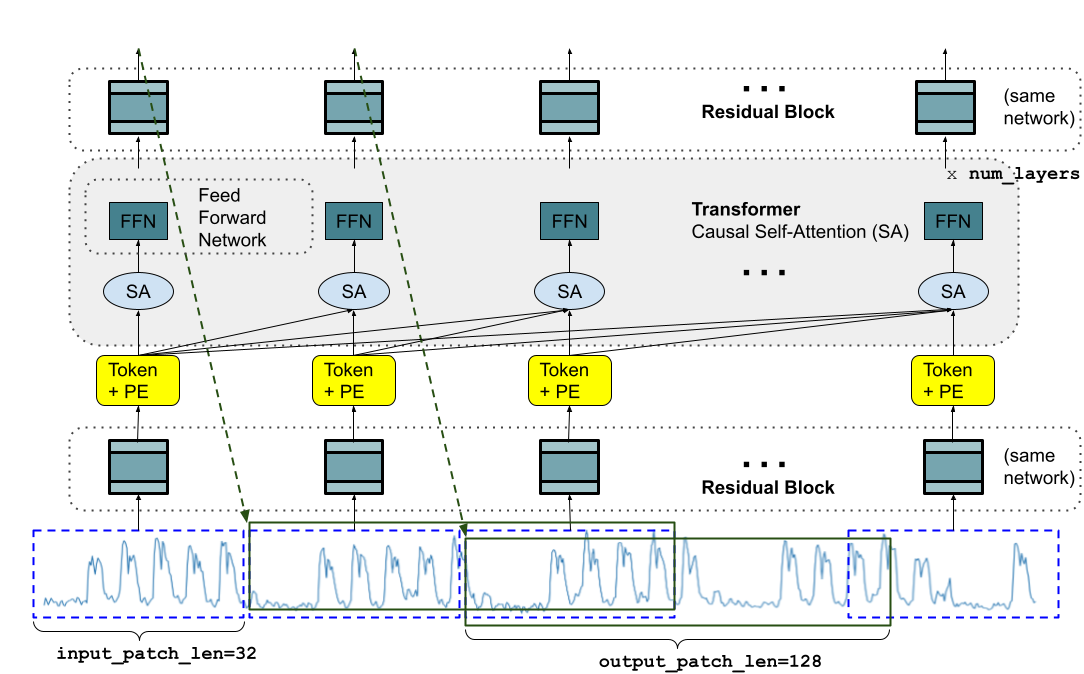
\includegraphics[width=0.75\linewidth]{fts_new_v2.png}
\caption{훈련 중 \ours~모델 아키텍처에 대한 그림을 제공합니다. 여기서는 입력 패치로 분할할 수 있는 특정 길이의 입력 시계열을 보여줍니다. 각 패치는 변환기 레이어의 모델 차원에 대한 잔차 블록(모델 정의에 정의된 대로)에 의해 벡터로 처리됩니다. 그런 다음 벡터는 위치 인코딩에 추가되고 $n_l$ 적층 변환기 레이어에 공급됩니다. SA는 self-attention(다중 헤드 인과 주의를 사용함)을 나타내며 FFN은 변환기의 완전 연결 레이어입니다. 그런 다음 출력 토큰은 잔여 블록을 통해 \texttt{output\textunderscore patch\textunderscore len} 크기의 출력에 매핑됩니다. 이는 지금까지 모델에서 확인한 마지막 입력 패치 이후의 시간 창에 대한 예측입니다.}
\label{fig:model}
\end{figure*}

{\bf 입력 레이어.} 입력 레이어의 작업은 시계열을 변환기 레이어에 대한 입력 토큰으로 전처리하는 것입니다. 먼저 입력을 겹치지 않는 연속 패치로 나눕니다. 그런 다음 각 패치는 Residual Block에 의해 \texttt{model\textunderscore 희미한} 크기의 벡터로 처리됩니다. 입력과 함께 바이너리 패딩 마스크 $\*m_{1:L}$도 제공합니다. 여기서 $1$은 $\*y_{1:L}$의 해당 입력이 무시되어야 함을 나타내고 그 반대의 경우도 마찬가지입니다. 잔여 블록은 본질적으로 ~\citep{das2023longterm}에 정의된 것과 유사한 건너뛰기 연결이 있는 하나의 숨겨진 레이어가 있는 MLP(Multi-layer Perceptron) 블록입니다.

% The mixture of experts implementation we use is identical to the top-2 gating using in~\citep{lepikhin2020gshard}. We shall see in Section~\ref{sec:emp} that the MoE layer helps the network adapt to different granularities. 

즉, 입력 $\*y_{1:L}$은 \texttt{input\textunderscore patch\textunderscore len}($p$) 크기의 패치로 분할됩니다. $j$번째 패치는 $\tilde{\*y}_j = \*y_{p(j-1)+1:pj}$으로 표시될 수 있습니다.  마찬가지로 마스크를 $\tilde{\*m}_j = \*m_{p(j-1)+1:pj}$으로 패치할 수도 있습니다. 그러면 후속 변환기 레이어에 대한 $j$번째 입력 토큰은 다음과 같이 표시될 수 있습니다.
\begin{align}
    \*t_j = \texttt{InputResidualBlock}(\tilde{\*y}_j\odot (1 - \tilde{\*m}_j)) + \texttt{PE}_j \label{eq:input}
\end{align}
여기서 $\texttt{PE}_j$은 원래 변환기 문서~\citep{vaswani2017attention}에 정의된 $j$번째 위치 인코딩을 나타냅니다. $N = \floor{L/p}$ 이러한 입력 토큰이 있습니다.

{\bf Stacked Transformer.} 우리 모델의 매개변수 대부분은 서로 겹쳐진 \texttt{num\textunderscore 레이어}($n_l$) 변환기 레이어에 있습니다. 이러한 각 계층에는 표준 다중 헤드 SA(Self-Attention)와 FFN(Feed-Forward Network)이 있습니다. 주요 하이퍼파라미터는 입력 토큰 $\*t_j$의 크기와 헤드 수(\texttt{num\textunderscore 헤드})와 동일한 \texttt{model\textunderscore 희미}입니다. FFN의 숨겨진 크기도 \texttt{model\textunderscore 희미}와 동일하게 설정했습니다. 우리는 각 출력 토큰이 시퀀스에서 앞에 오는 입력 토큰(해당 입력 토큰 포함)에만 주의를 기울일 수 있다는 인과적 주의를 사용합니다. 이는 방정식으로 설명할 수 있습니다.
\begin{align*}
    \*o_j = \texttt{StackedTransformer} ((\*t_1,\dot{m}_1), & \cdots, (\*t_{j},  \dot{m}_j ) ), \numberthis \label{eq:stacked}
\end{align*}
모든 $j \in [N]$에 대해. $\dot{m}_j$은 $\min\{\*m_{p(j-1)+1:pj}\}$으로 정의된 $j$번째 토큰에 대한 마스킹 표시기입니다. 즉, 패치에 마스킹되지 않은 시점이 있는 경우 해당 토큰은 마스킹되지 않은 것으로 표시됩니다. 완전히 가려진 모든 패치에는 원인적 self attention이 적용되지 않습니다.

% \begin{remark}
% \label{rem:padding}
% It might seem that with the above architecture we can only support context lengths that are multiples of \texttt{input\textunderscore patch\textunderscore len} ($p$). However, with a simple use of padding we can support any context length ranging from 1 to maximum training context length. We supply a binary padding mask $\*m_{1:L}$ where $1$ denotes that the corresponding input in $\*x_{1:L}$ should be ignored and vice-versa. Then $\tilde{\*x}_j$ can be pointwise multiplied by $1 - \*m_{p(j-1):pj}$ before feeding it to Eq.~\eqref{eq:input}. Moreover patches that are completely masked out can be excluded from the attention in Eq.~\eqref{eq:stacked}.
% \end{remark}

{\bf 출력 레이어.} 남은 작업은 출력 토큰을 예측에 매핑하는 것입니다. 우리는 디코더 전용 모드로 훈련합니다. 즉, 각 출력 토큰은 해당하는 마지막 입력 패치를 따르는 시계열 부분을 예측할 수 있어야 합니다. 이는 ~\citep{radford2019language}과 같은 널리 사용되는 대규모 언어 모델에 일반적입니다. 그러나 시계열 기초 모델의 주요 차이점 중 하나는 입력 패치 길이가 출력 패치 길이와 같을 필요가 없다는 것입니다. 즉, 지금까지 본 입력 패치의 인코딩된 정보를 기반으로 시계열의 더 큰 덩어리를 예측할 수 있어야 합니다. 출력 패치 길이를 \texttt{output\textunderscore patch\textunderscore len}($h$)으로 설정합니다. 우리는 또 다른 잔여 블록을 사용하여 출력 토큰을 예측에 매핑합니다. 이는 다음과 같이 설명될 수 있습니다.
\begin{align}
    \hat{\*y}_{pj+1: pj + h} = \texttt{OutputResidualBlock} \left( \*o_j \right). \label{eq:output}
\end{align}

따라서 $\*y_{1:pj}$의 모든 데이터를 $\*o_j$으로 인코딩하고 이를 사용하여 후속 $h$ 시점 ​​$\*y_{pj+1: pj + h}$을 예측합니다. 이는 하나의 훈련 미니 배치의 모든 패치에 대해 수행됩니다.

{\bf 손실 함수.} 이 작업에서는 점 예측에 중점을 둡니다. 따라서 MSE(Mean Squared Error)와 같은 학습 중에 포인트 예측 손실을 사용할 수 있습니다. 훈련 중 최소화되는 손실은 다음과 같이 표현될 수 있습니다.
\begin{align}
    \texttt{TrainLoss} = \frac{1}{N}\sum_{j=1}^{N} \mathrm{MSE}\left(\hat{\*y}_{pj+1: pj + h}, \*y_{pj+1: pj + h}\right).
\end{align}

확률적 예측에 관심이 있는 경우 각 출력 패치에 대해 여러 개의 출력 헤드를 갖는 것이 쉽습니다. 각 헤드는 ~\citep{wen2017multi}과 같이 별도의 분위수 손실을 최소화합니다. 또 다른 접근법은 확률 분포군의 로짓을 출력하고 확률적 예측에 대한 최대 우도 손실을 최소화하는 것입니다~\citep{awasthi2021benefits,salinas2020deepar}.

{\bf 훈련.} 우리는 시계열 및 시계열에 대한 모든 창을 통과하는 디코더 전용 방식의 표준 미니 배치 경사하강법을 사용하여 모델을 훈련합니다. 유일한 비표준 부분은 훈련 중에 마스크를 샘플링하는 방식입니다. 배치의 각 시계열에 대해 $0$과 $p-1$ 사이에서 임의의 숫자 $r$을 샘플링합니다. 그런 다음 $\*m_{1:r} = 1$을 설정하고 나머지는 0으로 설정합니다. 즉, \rev{out}을 첫 번째 입력 패치의 일부로 마스크합니다. 그러나 이는 1부터 최대 훈련 컨텍스트 길이까지 모든 입력 컨텍스트 길이를 포괄하는 데 충분합니다. 아래 예를 사용하여 이를 설명합니다.

최대 컨텍스트 길이가 512이고 $p=32$이라고 가정합니다. 그런 다음 $r=4$이 첫 번째 패치($\*o_1$)를 본 후의 출력 예측이 $28=32-4$ 시점을 본 후 예측하도록 최적화되고, 다음 패치($\*o_2$)의 출력이 $28+32$ 시점을 본 후 예측하도록 최적화되는 식입니다. 이러한 모든 $r$에 대해 이 인수가 반복되면 모델은 $512$까지 가능한 모든 컨텍스트 길이를 확인합니다.

{\bf 추론.} 훈련된 네트워크는 대규모 언어 모델과 유사한 자동 회귀 디코딩을 사용하여 \textit{any} 범위에 대한 예측을 생성하는 데 사용될 수 있습니다. $\*y_{1:L}$ 입력이 주어지면(단순화를 위해 $L$이 $p$의 배수라고 가정) 먼저 $\hat{\*y}_{L+1: L + h}$을 예측할 수 있습니다. 그런 다음 연결된 벡터 $\tilde{\*y}_{1:L+h} = [\*y_{1:L}; \hat{\*y}_{L+1: L + h}]$을 네트워크에 대한 입력으로 사용하여 다음 출력 패치 예측 $\hat{\*y}_{L+h+1: L + 2h}$ 등을 생성할 수 있습니다. $L$이 $p$의 배수가 아닌 경우 간단히 0을 추가하여 $p$의 배수로 만들고 마스크의 해당 항목을 1로 표시합니다.

%We name our model \textbf{Pre}trained \textbf{D}e\textbf{c}oder for \textbf{T}ime-series (\ours).
%We name our \textbf{T}ime-\textbf{s}eries \textbf{F}oundation \textbf{M}odel as \ours.

\section{사전학습 세부 사항}
\label{sec:pretrain}

우리는 배포된 모델을 통해 제공하려는 예측 사용 사례를 이상적으로 포착하는 다양한 도메인, 추세 및 계절성 패턴과 시간 세분성을 나타내는 대량의 시간 데이터를 사전 학습 코퍼스에 포함하기를 원합니다. 기초 모델을 교육하는 데 필요한 데이터의 양과 다양성을 충족하는 대규모 시계열 데이터 세트를 찾는 것은 어렵습니다. 우리는 Google 트렌드, Wiki 페이지뷰 통계 및 합성 시계열이라는 세 가지 주요 소스에서 모델을 훈련하는 데 사용되는 대량의 데이터를 소싱하여 이 문제를 해결합니다. 요약하면 주요 데이터 소스는 다음과 같습니다.

{\it Google Trends.} Google Trends~\footnote{\url{https://trends.google.com}}는 수백만 개의 검색어에 대한 시간 경과에 따른 검색 관심도를 파악합니다. 우리는 2007년부터 2022년까지 15년 동안의 검색 관심도를 기준으로 약 22,000개 정도의 헤드 쿼리를 선택합니다. 이러한 헤드 쿼리를 넘어서는 시계열은 50\%보다 희박해집니다. 우리는 시간별, 일별, 주별, 월별 세부 단위로 이러한 쿼리에 대한 시간 경과에 따른 검색 관심도를 다운로드하여 데이터 세트를 구성합니다. 날짜 범위는 시간별의 경우 2018년 1월부터 2019년 12월까지이고 기타 세부사항의 경우 2007년 1월부터 2021년 12월입니다.  추세 데이터 세트는 대략 \rev{0.5B} 시점에 해당합니다.

{\it Wiki Pageviews.} Wiki Pageviews~\footnote{\url{https://en.wikipedia.org/wiki/Wikipedia:Pageview_statistics}}는 모든 Wikimedia 페이지의 시간별 보기를 캡처합니다. 2012년 1월부터 2023년 11월까지의 모든 페이지 조회수 데이터를 다운로드하고, 페이지별 조회수를 시간별, 일별, 주별, 월별 단위로 정리 및 집계하고, 0이 너무 많은 페이지 조회 시계열을 필터링합니다. 최종 자료에는 대략 \rev{300B} 시점이 포함됩니다.

{\it 합성 데이터.} 사전 학습 데이터의 또 다른 주요 구성 요소는 합성 출처입니다. 우리는 ARMA~\citep{mckenzie1984general} 프로세스, 계절 패턴(서로 다른 주파수의 사인과 코사인의 혼합), 추세(선형, 몇 가지 변화 지점이 있는 지수형) 및 계단 함수에 대한 생성기를 만듭니다. 합성 시계열은 이러한 프로세스 중 하나 이상을 추가로 조합한 것일 수 있습니다. 우리는 각각 길이가 2048개 시점인 3M 합성 시계열을 생성합니다. 합성 데이터 생성에 대한 자세한 내용은 부록~\ref{app:syn}에 나와 있습니다.

{\it 기타 실제 데이터 소스.} Wiki 및 추세 데이터와 함께 공개적으로 사용 가능한 여러 데이터 세트의 시계열도 사전 학습 코퍼스에 추가합니다. M4 데이터 세트~\citep{makridakis2022m5}, 시간별 및 15분 전기 및 시간별 교통 데이터 세트(~\citep{zhou2021informer} 참조)의 모든 세부사항을 추가합니다. 또한 ~\citep{zhou2021informer}의 평가에 사용되는 10분 단위 날씨 데이터세트를 추가합니다. M4는 총 약 100,000개의 시계열로 세분성이 잘 혼합되어 있습니다. 교통 및 전기는 각각 수만 개의 시점을 갖는 $>$ 800 및 $>$ 300 시계열을 포함하는 대규모 장기 예측 데이터 세트입니다. 또한 ~\citep{libcitylong}의 15분 단위 트래픽 시계열을 모두 추가합니다.


\begin{table}[!ht]
    \centering
    \caption{TimesFM 사전 훈련 데이터 세트의 구성.}
    % \resizebox{0.\textwidth}{!}{
    \begin{tabular}{llrr}
    \toprule
    \multicolumn{1}{c}{Dataset} & \multicolumn{1}{c}{Granularity} & \multicolumn{1}{c}{\# Time series} & \multicolumn{1}{c}{\# Time points} \\ \midrule
    Synthetic & & 3,000,000 & 6,144,000,000  \\
    Electricity & Hourly & 321 & 8,443,584  \\
    Traffic & Hourly & 862 & 15,122,928  \\
    날씨~\citep{zhou2021informer} & 10분 & 42 & 2,213,232  \\
    파보리타 세일 & Daily & 111,840 & 139,179,538  \\
    리브시티~\citep{libcitylong} & 15분 & 6,159 & 34,253,622  \\
    M4 시간당 & Hourly & 414 & 353,500  \\
    M4 매일 & Daily & 4,227  & 9,964,658  \\
    M4 월간 & Monthly & 48,000 & 10,382,411  \\
    M4 분기별 & Quarterly & 24,000 & 2,214,108  \\
    M4 연간 & Yearly & 22,739 & 840,644  \\
    매시간 위키 & Hourly & 5,608,693 & 239,110,787,496  \\
    위키 데일리 & Daily & 68,448,204 & 115,143,501,240  \\
    위키 주간 & Weekly & 66,579,850 & 16,414,251,948  \\
    월간 위키 & Monthly & 63,151,306 & 3,789,760,907  \\
    시간별 동향 & Hourly & 22,435 & 393,043,680  \\
    일일 트렌드 & Daily & 22,435 & 122,921,365  \\
    주간 동향 & Weekly & 22,435 & 16,585,438  \\
    월간 동향 & Monthly & 22,435 & 3,821,760 \\
    \bottomrule
    \end{tabular}
    % }
    \label{tab:train_data}
\end{table}
{\bf 데이터 세트 혼합 및 훈련.} 모든 세분성 \rev{및 데이터 세트}에 충분한 가중치를 부여하는 것을 목표로 하는 이러한 데이터 세트에 대한 혼합 분포에 대해 훈련합니다. 학습 로더는 \rev{80@P4@@} 실제 데이터와 \rev{20\%} 합성을 샘플링하며, 실제 데이터 혼합은 그룹에 시간별 + 시간별, 일별, 주별 및 월별 데이터 세트에 동일한 가중치를 제공합니다.
시계열 길이가 허용할 때마다 최대 컨텍스트 길이 512로 훈련합니다. 주간 단위로 보기에는 충분히 긴 시계열이 없습니다. 따라서 최대 컨텍스트 길이인 256이 사용됩니다. 같은 이유로 $\geq$ 월별 세분성 데이터를 학습하는 동안 최대 컨텍스트 길이 64가 사용됩니다. 또한 가역적 인스턴스 정규화 ~\citep{kim2021reversible}의 표준 정규화 부분만 사용합니다. 즉, 각 시계열의 컨텍스트는 컨텍스트의 첫 번째 입력 패치의 컨텍스트 평균 및 표준 편차에 따라 조정됩니다.


\begin{figure*}[!ht]
  \centering
  \begin{subfigure}[b]{0.3\textwidth}
     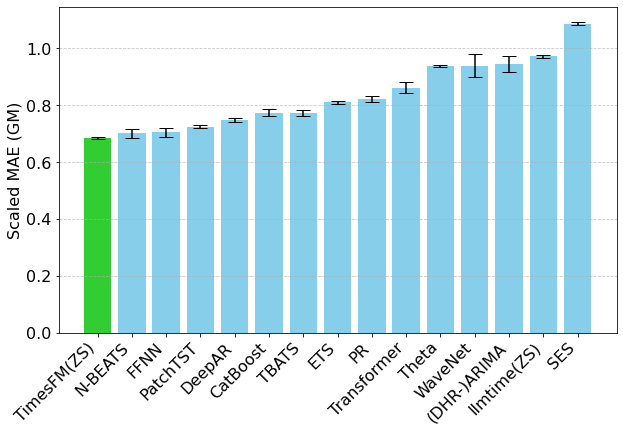
\includegraphics[width=\textwidth]{monash_mae_gm.png} % 'placeholder1'을 이미지 파일 이름으로 바꾸세요.
     \caption{\scriptsize{\rev{Monash Archive}~\citep{godahewa2021monash}}}
     \label{fig:monash_mae}
  \end{subfigure}
  \hfill % 하위 그림 사이에 약간의 공백을 추가합니다.
  \begin{subfigure}[b]{0.3\textwidth}
     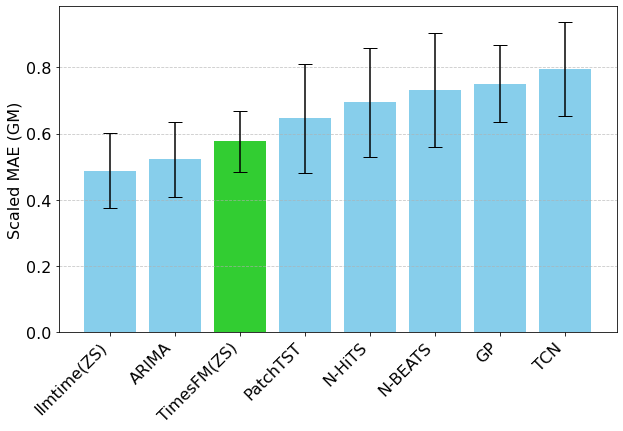
\includegraphics[width=\textwidth]{darts_chart_200m_gm_final.png} % 'placeholder2'를 이미지 파일 이름으로 바꾸세요.
     \caption{\scriptsize{\rev{Darts}~\citep{herzen2022darts}}}
     \label{fig:darts}
  \end{subfigure}
  \hfill % 하위 그림 사이에 약간의 공백을 추가합니다.
  \begin{subfigure}[b]{0.3\textwidth}
     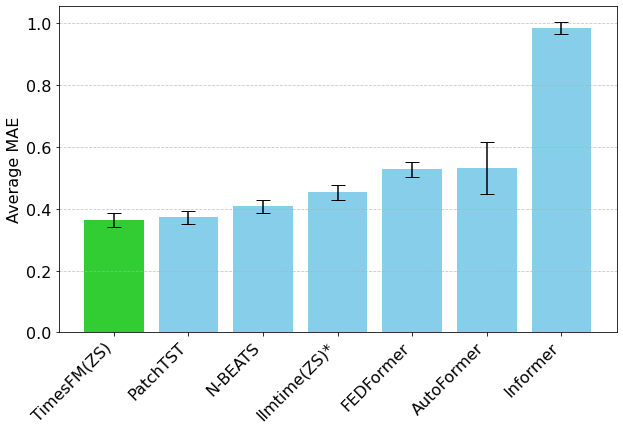
\includegraphics[width=\textwidth]{autoformer_chart_200m_final.png} % 'placeholder3'을 이미지 파일 이름으로 바꾸세요.
     \caption{\scriptsize{ETT (Horizons 96 and 192)~\citep{zhou2021informer}}}
     \label{fig:informer}
  \end{subfigure}
\caption{우리는 세 가지 데이터 세트 그룹의 평균 성능을 보고합니다. 모든 수치에서 측정항목이 낮을수록 더 좋고 오류 막대는 하나의 표준 오류를 나타냅니다. 기준선 중에서 \rev{만} \ours~및 llmtime은 제로샷입니다. (a)에서는 Monash 데이터세트에 대한 결과를 보고합니다. \rev{데이터세트의 규모가 다르기 때문에 순진한 기준선의 MAE로 조정된 MAE의 기하 평균(GM)을 사용합니다}. \ours~가 상위 모델임을 알 수 있습니다. (b)에서는 Darts 벤치마크에서 유사한 규모의 MAE를 보고합니다. \ours~는 이 경우 ARIMA 및 llmtime인 최고 성능 방법의 중요성 내에 있습니다. 이러한 데이터 세트에는 각각 하나의 시계열이 있으므로 통계 방법은 딥 러닝 방법과 경쟁력이 있습니다. 마지막으로 (c)에서 우리는 4개 ETT 데이터세트, 즉 총 8개 작업에 대한 96개 및 192개 지평선 예측 작업에 대한 \rev{평균} MAE를 보고합니다. \ours~와 PatchTST가 가장 성능이 좋은 모델입니다.}
  \label{fig:all_bar_charts}
\end{figure*}

\section{실증 결과}
\label{sec:emp}

우리는 각 그룹의 최고 성능 기준과 비교하여 잘 알려진 공개 데이터세트의 세 그룹에 대한 제로샷 설정에서 모델을 평가합니다. 이러한 데이터 세트는 사전 훈련 데이터에서 의도적으로 제외되었습니다. 우리는 \textit{single} 사전 훈련된 모델이 각 특정 작업에 대해 기준선이 특별히 훈련되거나 조정된 경우에도 벤치마크에서 기준선 모델의 성능에 근접하거나 능가할 수 있음을 보여줍니다. 그 후, 우리는 아키텍처에서 이루어진 다양한 선택을 정당화하는 절제 연구를 수행합니다.

\subsection{제로샷 평가}
\label{sec:zeroshot}
모델 성능을 벤치마킹하기 위해 일반적으로 사용되는 세 가지 예측 그룹을 선택합니다.
다양한 도메인, 크기, 세분성 및 지평선 길이를 포괄하는 데이터 세트: Darts~\citep{herzen2022darts}, Monash~\citep{godahewa2021monash} 및 Informer 데이터 세트~\citep{zhou2021informer}, 다른 기준에 대해 기초 모델의 일반화 능력을 테스트합니다.

모든 경우에 우리는 \rev{표준 테스트 분할 또는 다른 문헌의 일반적인 테스트 분할을 사용하여} 데이터세트의 공식 측정항목 및 확장에 대한 성능을 보고합니다. 아래에 결과 요약을 제시합니다. 자세한 내용은 부록~\ref{app:moreexp}에서 확인할 수 있습니다. 부록~\ref{app:moremodels}에서 모델에 대한 하이퍼 매개변수 및 기타 세부 정보를 제공합니다.

% In order to present the average results on each dataset groups we need to aggregate the metrics in such a way that they reflect the hardness of the individual datasets and also not be skewed by different scales in each dataset. Therefore, we report the percentage improvement of the algorithms over a \textit{Naive} method that outputs the constant prediction set to the mean of the context window. The percentage improvements are then averaged across all the datasets in each group.

{\bf Monash~\citep{godahewa2021monash}.} Monash 아카이브는 금융, 수요 예측, 날씨 및 교통을 포함한 도메인과 분에서 수년까지의 세부사항을 포괄하는 다양한 훈련 및 예측 길이의 30개 데이터세트 모음입니다. 아카이브는 지수 평활화(ETS) 및 ARIMA와 같은 여러 통계 기준과 CatBoost~\citep{prokhorenkova2018catboost}, DeepAR~\citep{salinas2020deepar} 및 WaveNet~\citep{oord2016wavenet}과 같은 감독 ML 기준에 대한 4가지 공식 측정항목을 보고합니다. llmtime~\citep{gruver2023large}에 이어 Monash Huggingface 저장소~\footnote{\url{https://huggingface.co/datasets/monash_tsf}}에서 시작하여 누락된 값이 포함된 데이터세트를 필터링합니다. 이로써 부록~\ref{app:monash}에 지정하는 18개의 데이터 세트가 남습니다.

이전 작업~\citep{gruver2023large}에 이어 4가지 공식 지표 중 평균 MAE 측면에서 성과를 보고합니다(부록~\ref{app:metrics} 참조). 데이터 세트의 규모가 엄청나게 다르기 때문에 각 데이터 세트에 대해 각 시계열의 컨텍스트에서 마지막 값을 지속적으로 예측하는 순진한 기준으로 달성한 측정 항목으로 측정 항목을 정규화합니다. 그런 다음 조정된 MAE가 모든 데이터세트에 걸쳐 평균화됩니다. Scaled Aggregation은 ~\citep{gruver2023large}에서도 사용되었습니다. \rev{그림~\ref{fig:monash_mae}에서는 정규화된 측정 항목에 대해 더 강력하므로 평균화에 기하 평균(GM)을 사용합니다~\citep{fleming1986not}. 또한 부록의 Figure~\ref{fig:all_bar_charts_am}에 산술 평균 기반 집계 측정항목을 보고합니다.}

모든 데이터세트에 걸쳐 평균 조정된 MAE가 표준 오차 막대와 함께 Figure~\ref{fig:monash_mae}에 표시됩니다. \ours~의 성능을 Monash에서 구현된 기본 모델과 특정 프롬프트 기법으로 GPT-3~\citep{radford2019language}을 사용하는 제로샷 llmtime~\citep{gruver2023large} 모델과 비교합니다. 제로샷 모델은 (\textbf{Z}ero-\textbf{S}hot)으로 표시됩니다. \rev{\ours~은 이러한 데이터 세트에 대해 교육한 적이 없지만 최고의 모델입니다. 약간 더 낫지만 N-BEATS만큼 중요하지만 DeepAR~\citep{salinas2020deepar}과 같은 심층 감독 모델보다 성능이 뛰어나고 llmtime의 성능이 25\%} 이상 향상됩니다.

{\bf Darts~\citep{herzen2022darts}.} 이는 흥미로운 계절성과 덧셈+곱셈 추세를 포함하는 8개의 일변량 데이터세트 모음입니다. 우리는 TCN~\citep{lea2016temporal}, N-HiTS~\citep{challu2022nhits} 및 N-BEATS~\citep{oreshkin2019n}과 같은 Darts 패키지에 구현된 여러 기준의 성능을 보고합니다. 이러한 모든 기준은 감독됩니다. 이전과 마찬가지로 GPT-3~\citep{radford2019language}을 사용하여 llmtime~\citep{gruver2023large}의 제로샷 예측 결과도 보고합니다. SM-GP~\citep{wilson2013gaussian} 및 ARIMA~\citep{mckenzie1984general}과 같은 ~\citep{gruver2023large}의 다른 감독 기준선도 추가됩니다.

부록~\ref{app:moreexp}의 각 개별 데이터 세트에 대한 MAE인 이 데이터 세트 그룹의 공식 측정항목을 보고합니다. 그림~\ref{fig:darts}에서는 Monash 데이터세트에서와 마찬가지로 8개 데이터세트 전체에 걸쳐 평균 확장된 MAE를 제시합니다. \ours~는 이 경우 llmtime 및 계절성 ARIMA인 최상의 모델의 통계적 유의성 내에 있습니다. 이 데이터 세트 그룹에는 8개의 개별 시계열만 있으므로 표준 오류가 날카롭지 않아 모델 간의 명확한 순서를 제공하지 않습니다. 또한 ARIMA의 경우 최상의 결과를 얻으려면 매개변수에 계절성을 올바르게 인코딩해야 하므로 수동 조정이 필요합니다. 또한 이러한 데이터 세트는 설명 목적으로 수많은 시계열 블로그 게시물에 사용되므로 llmtime의 데이터 오염을 배제할 수 없습니다.


{\bf Informer~\citep{zhou2021informer}.} Informer 데이터 세트는 다양한 감독 장기 예측 방법을 벤치마킹하는 데 널리 사용되었습니다. 이러한 데이터 세트 중 일부는 사전 훈련에 사용되므로 $1$ 시간 및 $15$ 분 단위로 2년 동안 변압기 온도와 관련된 이 컬렉션의 다른 데이터 세트(ETTm1, ETTm2. ETTh1 및 ETTh2)에 중점을 둡니다. 긴 지평선 기준선은 일반적으로 llmtime~\citep{gruver2023large} 평가를 위해 수백만 개의 토큰에 해당하고 비용이 너무 많이 드는 테스트 세트에 대한 롤링 검증 결과를 보고합니다. 따라서 llmtime 이후 마지막 테스트 창에서 모든 메서드를 비교합니다. 또한 결과가 표준 정규화된 데이터 세트(훈련 부분의 통계 사용)에 보고되므로 이러한 데이터 세트에 대한 MAE를 직접 평균하는 것이 합리적입니다.

우리는 모든 방법에 대해 컨텍스트 길이가 512인 경우 수평선 길이 96과 192를 예측하는 작업을 고려합니다. 8개 작업(각각 두 개의 지평선이 있는 4개의 데이터 세트)에 대한 평균 MAE가 그림~\ref{fig:darts}에 표시됩니다. \ours~는 최고의 성능을 발휘하며 감독된 PatchTST~\citep{nie2022time} 기준선(최첨단 장기 심층 예측 방법)이 그 의미를 갖습니다. 다른 긴 지평선 방법은 이러한 데이터 세트를 훈련받았음에도 불구하고 상당히 더 나쁩니다. llmtime은 FEDFormer보다 우수하지만 통계적 유의성이 있어 PatchTST보다 나쁩니다.

\rev{부록~\ref{app:syn_exp}에 기준선과 함께 예측의 시각적 예시를 제시합니다.}


% {\bf Visualizing Forecasts.} Next, we conduct a visual inspection of the forecasts generated by \ours, first on some synthetic examples and then on the benchmark datasets.

% In Figure~\ref{fig:viz-syn-4p} we show 4 different synthetic curves: (1) sum of 5 sine curves of different periods, (2) a sine curve linearly scaled, (3) a sine curve with a linear trend, and (4) minimum of two sine curves with a linear trend. Our results suggests that \ours~picks up the trend and seasonal components readily interpretable by humans, while ARIMA and (to a lesser extent) llmtime fail in some of the instances.

% As illustrated in Figure~\ref{fig:visualization-4p}, \ours~also effectively captures these subtle characteristics within both the trend and seasonal patterns of the depicted real world time-series. For instance, in the Air Passenger dataset, \ours~correctly captures the amplitude increase with trend --this is also reflected by the fact that it attains the best MAE on this dataset (see Table~\ref{tab:darts}). In the traffic hourly example on the left, it can be seen that \ours~can correctly identify the seasonal peaks even in the presence of outliers in the context, while llmtime is thrown off.

% More examples are presented in Appendix~\ref{app:moreexp}.

% \begin{figure}[!ht]
%     \centering
%     
\includegraphics[width=1.0\linewidth]{figures/syn_4.png}
% \caption{Forecasts visualized on synthetic curves. The bottom row plots zoom in on the prediction horizon for the sake of clarity.}
% \label{fig:viz-syn-4p}
% \end{figure}

% \begin{figure}[!ht]
%     \centering
%     
\includegraphics[width=1.0\linewidth]{figures/visualization-4p-darts-monash.png}
% \caption{Forecasts visualized on Darts and Monash. The bottom row plots zoom in on the prediction horizon for the sake of clarity.}
% \label{fig:visualization-4p}
% \end{figure}

\subsection{절제 실험}
\label{sec:ablation}

\begin{figure*}[!ht]
    \centering
    \begin{subfigure}[b]{0.4\textwidth}
       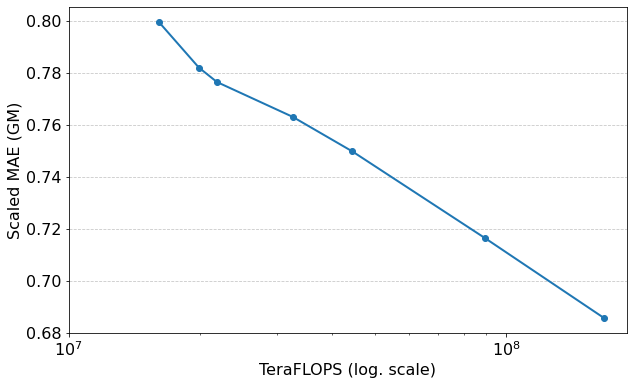
\includegraphics[width=\textwidth]{scaling_flops.png} % 'placeholder1'을 이미지 파일 이름으로 바꾸세요.
       \caption{17M, 70M 및 200M의 세 가지 모델 크기에 걸쳐 FLOPS의 함수로 Monash 데이터 세트의 확장된 MAE(GM)입니다. 처음 4개 지점은 17M 및 70M 체크포인트에서 나온 것이고 마지막 3개 지점은 200M에서 나온 것입니다.}
       \label{fig:scale}
    \end{subfigure}
    \hfill % 하위 그림 사이에 약간의 공백을 추가합니다.
    \begin{subfigure}[b]{0.4\textwidth}
       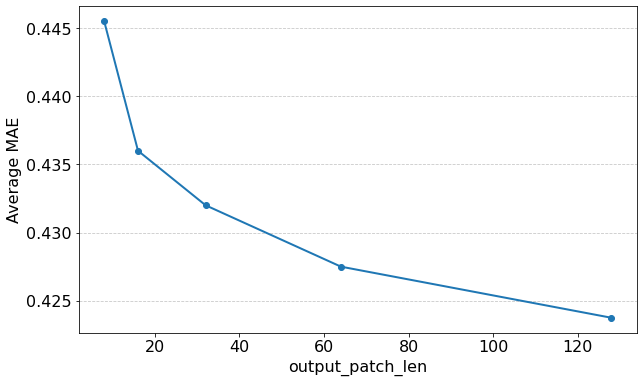
\includegraphics[width=\textwidth]{op_len_new.png} % 'placeholder2'를 이미지 파일 이름으로 바꾸세요.
       \caption{~\citep{zhou2021informer}의 원래 테스트 세트에서 ETT 데이터세트의 미래 512단계를 예측하는 작업에 대한 출력 패치 길이와 관련된 제거입니다. 우리는 4개의 ETT 데이터 세트 전체에 대한 평균을 보고합니다.}
       \label{fig:auto}
    \end{subfigure} \\
    \begin{subfigure}[b]{0.4\textwidth}
       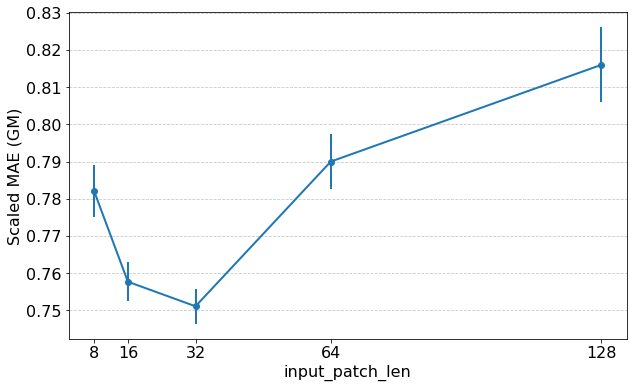
\includegraphics[width=\textwidth]{ip_len_abl_detailed.png} % 'placeholder3'을 이미지 파일 이름으로 바꾸세요.
       \caption{다양한 입력 패치 길이에 대한 Monash 데이터 세트의 70M 모델에 대한 확장된 MAE(GM)입니다. 또한 하나의 표준 오류를 나타내는 오류 막대를 표시합니다.}
       \label{fig:iplen}
    \end{subfigure}
    \hfill % 하위 그림 사이에 약간의 공백을 추가합니다.
    \begin{subfigure}[b]{0.4\textwidth}
        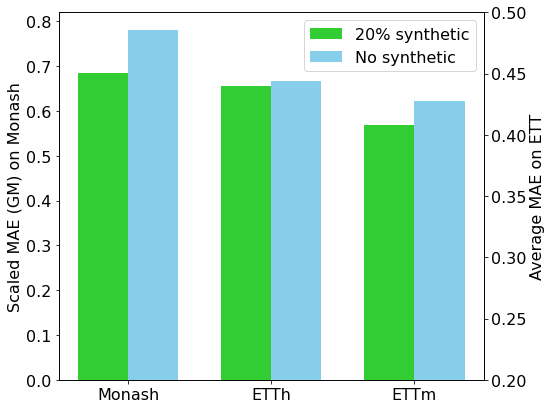
\includegraphics[width=\textwidth]{dataset_abl_new.png} % 'placeholder3'을 이미지 파일 이름으로 바꾸세요.
        \caption{왼쪽은 Monash의 평균 확장 MAE이고 오른쪽은 ETT 데이터세트의 평균 MAE입니다. 합성 데이터가 있는 모델과 없는 200M 모델의 성능을 비교합니다.}
        \label{fig:tbbbb}
     \end{subfigure}
  \caption{다양한 디자인 선택에 관한 절제 연구.}
    \label{fig:datasets-abl}
  \end{figure*}

다음으로, 모델 아키텍처에 대한 설계 결정을 알리는 여러 가지 절제 연구를 수행합니다.

{\bf 확장.} 모델의 매개변수 수와 관련된 성능 곡선은 LLM의 맥락에서 예리하게 연구된 영역이었습니다. ~\citep{kaplan2020scaling}은 언어 모델의 매개변수 수와 다운스트림 성능 사이의 관계와 같은 거듭제곱 법칙을 확립했습니다. 즉, 매개변수 수가 많을수록 성능이 향상됩니다. 그러나 ~\citep{hoffmann2022training}은 훈련 데이터 세트에서 사용 가능한 토큰 수를 기반으로 최적 모델을 계산하여 훈련하는 방법을 규정하는 보다 미묘한 확장 법칙을 확립했습니다.

\rev{우리는 17M, 70M 및 200M 크기의 \ours~모델 3개를 동일한 사전 훈련 데이터 세트를 사용하여 4096의 전역 배치 크기로 150만 반복까지 훈련하는 예비 확장 연구를 수행합니다. 그런 다음 다양한 모델 실행에서 다양한 수의 FLOPS(부동 소수점 연산)를 나타내는 체크포인트를 수집합니다. 그런 다음 Monash의 Scaled MAE(GM) 성능을 FLOPS의 함수로 그림~\ref{fig:scale}에 표시합니다. 이는 이제 LLM에서 확장 연구를 수행하는 표준 방법입니다(~\citep{gu2023mamba}과 같은 최근 작업 참조). FLOPS 수(로그 스케일)에 따라 오류가 단조롭게 감소하는 것을 분명히 볼 수 있습니다. \rev{모든 실험은 16개의 텐서 코어가 있는 TPUv5e\footnote{\url{https://cloud.google.com/tpu/docs/v5e-training}} 설정에서 수행되었습니다. 2억 모델의 경우 설정에서 150만 번의 반복을 완료하는 데 2일이 걸립니다.}}

% \begin{figure}[!ht]
%     \centering
%     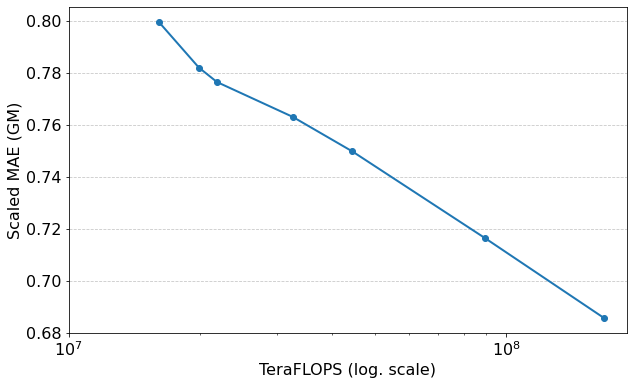
\includegraphics[width=0.8\linewidth]{scaling_flops.png}
% \caption{\rev{Scaled MAE (GM) on Monash datasets as a function of FLOPS across three model sizes 17M, 70M and 200M. The first 4 points are from 17M and 70M checkpoints while the last 3 are from 200M.}}
% \label{fig:scale}
% \end{figure}

{\bf Autoregressive Decoding.} 최근 장기 예측 작업에서~\citep{zeng2022transformers,nie2022time,das2023longterm} 디코더에서 한 번에 전체 예측 범위를 직접 예측하는 것이 긴 범위 벤치마크에서 자동 회귀 디코딩보다 더 나은 결과를 얻을 수 있다는 것이 관찰되었습니다. 기초 모델의 경우 추론 시간 이전에는 작업의 수평 길이를 알 수 없으므로 매우 긴 수평에서는 원샷 디코딩이 불가능할 수 있습니다. 그러나 앞서 언급했듯이 \texttt{output\textunderscore patch\textunderscore len}을 \texttt{input\textunderscore patch\textunderscore len}보다 길게 유지하면 자동 회귀 단계를 줄일 수 있습니다. 이는 LLM과 상당히 다른 \ours 설계의 주요 결정 중 하나였습니다. \rev{이를 보여주기 위해 우리는 ETT 테스트 세트의 원래 롤링 검증 작업에서 ETT 데이터세트에 대해 미래의 512개 시간 단계를 예측하는 작업을 선택합니다~\citep{zhou2021informer}. 그림~\ref{fig:auto}에서는 8에서 128까지 다양한 output\textunderscore patch\textunderscore len을 갖는 모델의 결과를 제시합니다. 우리는 output\textunderscore patch\textunderscore len에서 평균 MAE의 단조로운 감소를 확인합니다.}

% \begin{figure}[!ht]
%     \centering
%     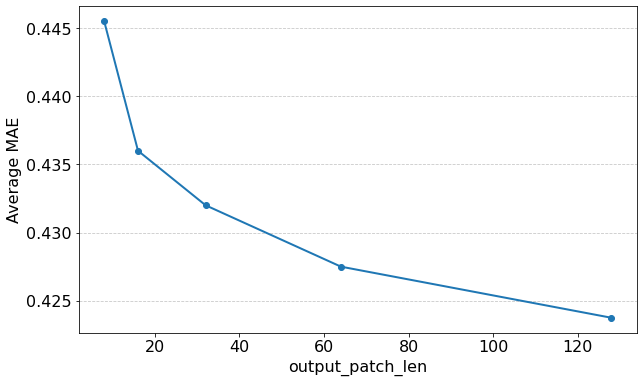
\includegraphics[width=0.7\linewidth]{op_len_new.png}
% \caption{Ablation with respect to output patch length for the task of predicting 512 steps into the future on ETT datasets on the original test set in~\citep{zhou2021informer}. We report the average across all 4 ETT datasets.}
% \label{fig:auto}
% \end{figure}

{\bf 입력 패치 길이.~} \texttt{input\textunderscore patch\textunderscore len}의 크기는 중요한 절충안을 나타냅니다. 일반적으로 값을 8에서 32로 늘리면 성능이 향상되지만 \texttt{input\textunderscore patch\textunderscore len}이 너무 높으면 모델이 디코더 전용 학습에서 인코더-디코더 스타일 학습으로 전환되기 때문에 비실용적입니다. 섹션~\ref{sec:model}의 "훈련" 단락에서는 모든 컨텍스트 길이를 지원하는 마스크 샘플링 전략을 설명합니다. 극단적인 경우 $p$이 최대 컨텍스트 길이로 설정되면 가능한 모든 컨텍스트 창을 1부터 최대 컨텍스트 길이까지 개별적으로 샘플링해야 하며 이는 인코더-디코더 스타일의 교육에 필요합니다.

\rev{그림~\ref{fig:iplen}에서는 평균 스케일링 MAE(GM) \ours(ZS) - \texttt{input\textunderscore patch\textunderscore len}이 8에서 128까지 다양한 Monash의 70M 모델을 보여줍니다. p=8 모델이 훈련하는 데 3배 느리더라도 두 모델 모두 약 1.5M 단계로 훈련되었습니다. $p=16,32$이 최고의 성능을 나타내는 것을 볼 수 있으며 양쪽 끝으로 갈수록 오류가 증가합니다. $p=32$ 모델은 $p=16$에 비해 학습 속도가 거의 두 배 빠르므로 신중한 선택이 됩니다.}

% \begin{figure}[!ht]
%     \centering
%     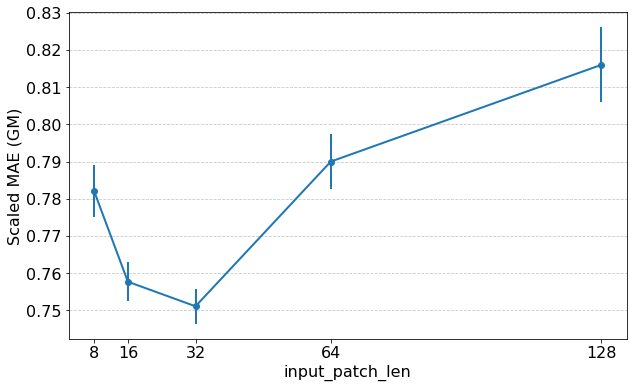
\includegraphics[width=0.7\linewidth]{ip_len_abl_detailed.png}
% \caption{Scaled MAE (GM) for our 70M models on Monash datasets for different input patch lengths. We also plot error bars denoting one standard error.}
% \label{fig:iplen}
% \end{figure}
{\bf 데이터세트 제거.}
\rev{다음으로 합성 데이터의 필요성을 보여드리겠습니다. 직관적으로, 실제 데이터 세트의 대부분은 시간별 데이터에 대한 24개 시점 기간과 같은 특정 주기적 패턴을 갖는 시간별, 일별 등과 같은 세분성을 일반적으로 발견했습니다. 이로 인해 모델이 과소대표된 주파수에 대해 잘 일반화되지 않을 수 있습니다. 혼합에 합성 데이터를 추가하지 않고 2억 모델을 훈련하고 Figure~\ref{fig:datasets-abl}에서 Monash 및 ETT 데이터 세트의 성능을 보여줍니다. Monash의 많은 데이터 세트가 분기별, 연간 또는 10분 등과 같은 세분성을 과소 표현했기 때문에 Monash의 성능 저하가 있음을 알 수 있습니다. 아마도 훨씬 더 매력적인 것은 ETT 데이터 세트에 대한 비교일 것입니다. 세분성이 잘 표현된 시간별 ETTh 데이터세트에서는 두 모델 사이에 거의 차이가 없음을 알 수 있습니다. 그러나 15분 ETTm 데이터세트의 경우 합성 데이터가 포함된 모델의 성능이 훨씬 더 좋습니다.}
% \begin{figure}[!ht]
%     \centering
%     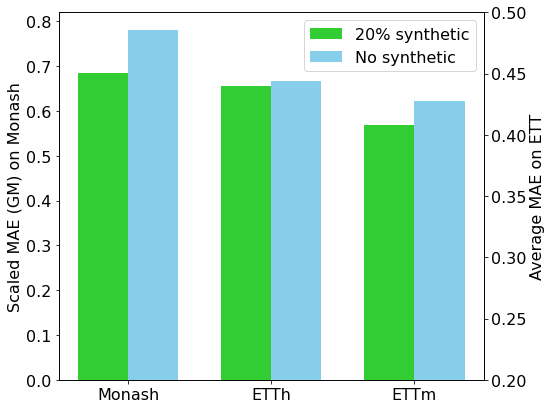
\includegraphics[width=0.8\linewidth]{dataset_abl_new.png}
% \caption{Average scaled MAE for Monash on the left and average MAE on ETT datasets on the right. We compare the performance of 200M model with and without the synthetic data.}
% \label{fig:datasets-abl}
% \end{figure}

\rev{우리는 부록~\ref{sec:finetuning}의 ~\citep{zhou2023one}과 동일한 설정에서 미세 조정 연구를 제공합니다. 여기서 우리 모델은 보고된 모든 데이터 세트의 모든 기준보다 더 나은 성능을 발휘합니다. 이는 다운스트림 작업에 대한 우리 모델의 유용성을 보여줍니다.}


% We are interested evaluating the performance of a single foundation model pretrained on a large time-series dataset on different target datasets never seen before by the model or, in other words, \textit{zero-shot evaluation}. To test the generalization performance of our baselines, we choose target datasets covering a variety of data domains, scales and time granularities. We will first discuss the pretraining and target datasets, along with the baselines we use. Then we demonstrate the (Z)ero-(S)hot performance of our model \ours(ZS) compared against state-of-the-art models trained directly on the target datasets. 
% %We also compare against other architectures pretrained on the same source datasets. 


% {\bf Target Datasets.} To benchmark our model's performance, we choose commonly used forecasting datasets of varying sizes that cover various domains, granularities, context lengths and horizon lengths, to test the generalization power of our foundation model against other baselines. The details are summarized in Table~\ref{tab:datasets}.

% \begin{table}
% \centering
% \resizebox{0.5\textwidth}{!}{%
% \begin{tabular}{lccccc}
% \toprule
% Dataset & \# Time-Series & Time Length & Granularity & Context & Horizon \\
% \midrule
% ETTm1 & 7 & 69680 & 15 Min. & 512 & 96 \\
% ETTm2 & 7 & 69680 & 15 Min. & 512 & 96 \\
% ETTh1 & 7 & 17420 & 1 Hour & 512 & 96 \\
% ETTh2 & 7 & 17420 & 1 Hour & 512 & 96 \\
% Wiki & 115084 & 803 & 1 Day & 256 & 56 \\
% ILI & 7 & 966 & 1 Week & 96 & 24 \\
% TourismL & 555 & 228 & 1 Month & 64 & 12 \\
% \bottomrule
% \end{tabular}%
% }
% \caption{Statistics and task definitions of the target datasets.}
% \label{tab:datasets}
% \end{table}

% {\it (Sub)Hourly.~} For 15 min. granularity we use the ETTm1, ETTm2 datasets and test all models on the task of predicting a horizon of 96 time-points after seeing a context of size 512. For hourly granularity, we choose the ETTh1, ETTh2 datasets and test all models on the same task as the 15 min. datasets. The datasets and the context, horizon pair have been widely used in long-term forecasting benchmarks~\citep{zhou2021informer, nie2022time}. Note that we used the more challenging original, unscaled versions of these datasets in order to test our model's zero-shot performance on time-series of different scales. 

% {\it Daily.~} For the daily granularity, we use the Wikipedia web-traffic dataset from the corresponding Kaggle competition~\footnote{\url{https://www.kaggle.com/code/muonneutrino/wikipedia-traffic-data-exploration}}. It has 115k time-series with over two years of data if we exclude the time-series with missing values. The dataset contains web-traffic to Wikipedia articles and the task is to predict the web-traffic (in $\log$ scale) on future dates. We choose a context length of 256 to predict a horizon of 56 days (8 weeks). This dataset has been used in prior multivariate forecasting papers such as like~\citep{sen2019think}.

% {\it Weekly.~} We use the ILI dataset\footnote{\url{https://gis.cdc.gov/grasp/fluview/fluportaldashboard.html}} that collects the number of patients and influenza-like illness ratio in a weekly
% frequency. We use a context length of 96 to predict 24 weeks into the future. This is one of the configurations used in long-term forecasting papers like~\citep{zhou2021informer}.

% {\it Monthly.~} We choose TourismL (Tourism Large)~\citep{wickramasuriya2019optimal} as one of the target datasets. It contains monthly tourist visit data in Australia that has been grouped into various regions. It consists of 555 time-series with very different scales. We choose the task of predicting a 12 month horizon given a context length of 64. 

% All the target datasets are divided into \texttt{train:validation:test} splits (periods) chronologically with the proportions being 7:1:2. We evaluate the models based on metrics resulting from rolling windows in the \texttt{test} period. Specifically, \ours(ZS) solely predicts in the \texttt{test} period as it has already been pretrained. The supervised learning models (per dataset) are trained on the \texttt{train} part with the hyper-parameters being tuned using the \texttt{validation} split. Then they predict in the \texttt{test} period for a head-to-head comparison with the zero-shot \ours(ZS). 

% {\bf Baselines.}  We  compare our model against three recently published state-of-the-art supervised forecasting models PatchTST~\citep{nie2022time}, TiDE~\citep{das2023longterm} and FEDFormer~\citep{zhou2022fedformer} as well as the popular N-BEATS~\citep{oreshkin2019n} and DeepAR models~\citep{salinas2020deepar}. Note that these models have already been shown~\citep{zhou2022fedformer,zhou2021informer} to be  superior to common statistical forecasting methods such as Prophet~\citep{taylor2018forecasting} and ARIMA;  hence we do not include them in our baselines. We train the above supervised models on the train split of each target dataset and measure their performance on the corresponding test split. For these supervised models we report the best metrics among models trained with and without date-derived features. See Appendix~\ref{app:moremodels} for the hyper-parameters used for each dataset. We compare our zero-shot metrics from \ours(ZS) to these state-of-the-art supervised metrics, which we denote by PatchTST(S), TiDE(S), N-BEATS(S), FEDFormer(S) and DeepAR(S) in our results below.

% %For all models we use standard normalization based reversible instance normalization (RevIN). Note that for foundation models learnable affine parameters for the instance normalization~\citep{kim2021reversible} is not possible as the inference dataset is not fixed a priori. Therefore we only use standard normalization RevIN for all the models in the interest of fair comparison. 

% In \ours(ZS), we set \texttt{input\textunderscore patch\textunderscore len=32},  \texttt{output\textunderscore patch\textunderscore len=128}. We train a model with about 225M parameters that uses 16 head multi-head attention in each transformer layer.

% {\bf Results.} In Table~\ref{tab:zsresults} we present the main results on all our target datasets. We report normalized metrics NRMSE and WAPE, that are proportional to MSE and MAE, and are defined (for each time-series) as
% \begin{align*}
%      \mathrm{NRMSE} \left(\*y_{L+1:L+H},  \hat{\*y}_{L+1:L+H}\right) &= \frac{\sqrt{\frac{1}{H} \norm{\*y_{L+1:L+H} - \hat{\*y}_{L+1:L+H}}_2^2}}{\frac{1}{H}  \norm{\*y_{L+1:L+H}}_1}, \\
%      \mathrm{WAPE} \left(\*y_{L+1:L+H},  \hat{\*y}_{L+1:L+H}\right) &= \frac{\frac{1}{H} \norm{\*y_{L+1:L+H} - \hat{\*y}_{L+1:L+H}}_1}{\frac{1}{H}  \norm{\*y_{L+1:L+H}}_1}.
% \end{align*}
%  The metrics in the table are across all time-series in the test period of the target datasets. The metrics are calculated over all rolling window (context, horizon) pairs that can be extracted from the test period. Note that FEDformer and DeepAR training was not able to scale to the Wiki dataset (the largest of our target datasets) and hence their metrics for Wiki in the table are left blank.
 
%  For each column in the table (corresponding to a metric computed for a dataset), we color-code the best performance by blue, the second-best performance by green, the worst  performances by red and the second-worst performance by orange. We observe that \ours(ZS) obtained uniformly good results (in the ballpark of the best supervised models) for a majority of the target datasets. In particular, \ours(ZS) obtained the best performance for the TourismL dataset, and close to the best performing models for Wiki, ETTh1 and ETTh2. It was among the best or second-best performing model for $8$ out of the $14$ columns in the table, and never among the worst two performing models in any column except one (where it was second-worst for NRMSE on ILI). This is particularly remarkable since we use a single, pretrained model evaluated in zero-shot manner on the target datasets, and are comparing here against state-of-the-art supervised baselines  trained separately on each of the datasets.  
 
% \begin{table*}[!ht]
% \centering
% \resizebox{\textwidth}{!}{%
% \begin{tabular}{lcc|cc|cc|cc|cc|cc|cc}
% \toprule
%  \multirow{2}{*}{Model} & \multicolumn{2}{c}{ETTh1} & \multicolumn{2}{c}{ETTh2} & \multicolumn{2}{c}{ETTm1} & \multicolumn{2}{c}{ETTm2} & \multicolumn{2}{c}{Wiki} & \multicolumn{2}{c}{ILI} & \multicolumn{2}{c}{TourismL} \\
% \cmidrule(lr){2-3} \cmidrule(lr){4-5} \cmidrule(lr){6-7} \cmidrule(lr){8-9} \cmidrule(lr){10-11} \cmidrule(lr){12-13} \cmidrule(lr){14-15}
%  & NRMSE & WAPE & NRMSE & WAPE & NRMSE & WAPE & NRMSE & WAPE & NRMSE & WAPE & NRMSE & WAPE & NRMSE & WAPE\\
% \midrule
% PatchTST(S) & \textbf{\best{0.656}} & 0.380 & 0.245 & 0.161 & \textbf{\best{0.571}} & \textbf{\best{0.307}} & \secondbest{0.180} & \secondbest{0.114} & \worst{0.115} & \worst{0.081} & \secondbest{0.414} & \secondbest{0.132} & 0.590 & 0.203 \\
% TiDE(S)  & \secondbest{0.663} & \textbf{\best{0.374}} & 0.245 & 0.161 & \secondbest{0.588} & 0.320 & 0.186 & 0.120 & \textbf{\best{0.103}} & \secondbest{0.070} & 0.455 & \textbf{\best{0.131}} & \secondbest{0.574} & \secondbest{0.194} \\
% N-BEATS(S) & \secondworst{0.687} & \secondworst{0.421} & \textbf{\best{0.235}} & \secondbest{0.152} & 0.608 & 0.320 & \textbf{\best{0.179}} & \textbf{\best{0.111}} & \textbf{\best{0.103}} & \textbf{\best{0.069}} & \textbf{\best{0.410}} & 0.137 & 0.666 & 0.213 \\
% FEDFormer(S) & 0.675 & 0.411 & \secondworst{0.294} & \secondworst{0.205} & \secondworst{0.635} & \secondworst{0.381} & \secondworst{0.240} & \secondworst{0.152} & - & - & 0.441 & \secondworst{0.164} & \worst{1.080} & \worst{0.266} \\
% DeepAR(S) & \worst{0.851} & \worst{0.468} & \worst{0.331} & \worst{0.228} & \worst{0.892} & \worst{0.453} & \worst{0.283} & \worst{0.177} & - & - & \worst{0.844} & \worst{0.534} & \secondworst{0.859} & \secondworst{0.264} \\
% \midrule
% \ours(ZS) & 0.672 & \secondbest{0.378} & \secondbest{0.238} & \textbf{\best{0.151}} & 0.591 & \secondbest{0.310} & 0.199 & 0.123 & \secondbest{0.107} & \secondbest{0.070} & \secondworst{0.477} & 0.152 & \textbf{\best{0.514}} & \textbf{\best{0.192}} \\
% \bottomrule
% \end{tabular}%
% }
% \caption{We present NRMSE and WAPE metrics for (S)upervised models and our (Z)ero-(S)hot model. The supervised models are trained, tuned and evaluated on the specific target datasets. \ours(ZS) metrics are reported on zero-shot performance i.e the model has never seen the target dataset prior to inference. The \best{best} number in each column is colored blue, and the \secondbest{second-best} number is colored green. The \worst{worst}  performing model metrics per column is colored red and the \secondworst{second-worst} is colored orange. It can be seen that the \ours(ZS) metrics are uniformly good across all datasets and was among the best or second-best performing model for $8$ out of the $14$ columns. We report standard errors for the supervised metrics in Table~\ref{tab:zsresults_full} in the appendix.}
% \label{tab:zsresults}
% \end{table*}

% \subsection{Ablation}
% \label{sec:ablation}
% Next, we perform several ablation studies that inform  the design decisions we made for our foundation model architecture.

% {\bf Different architectures on same pretraining data.} 
% % PatchTST~\citep{nie2022time} and N-BEATS~\citep{oreshkin2021meta} have been both shown to be able to meta-learn across datasets. Therefore, we train these models on the same pretraining dataset as \ours(ZS) and measure their zero-shot performance on the target datasets. 
% \citep{nie2022time} have shown that PatchTST can be used to learn semi-supervised representations of time-series. Similarly ~\citep{oreshkin2021meta} have shown that the N-BEATS architecture can be used for transfer learning in time-series. Therefore, we also consider pre-training a foundation model based on the  PatchTST and N-BEATS architecture using the same pretraining dataset, and evaluate them in a zero-shot manner on the target datasets, similar to \ours(ZS). These baselines will be denoted by PatchTST(ZS) and N-BEATS(ZS). Note that N-BEATS(ZS) was restricted to training and inference with a fixed context length on account of being a MLP model. 

% The results are shown in Table~\ref{tab:arch}. It can be seen that \ours(ZS) performs better than or similar to  PatchTST(ZS) on ETTh1, ETTh2, ETTm2, Wiki and TourismL, but we are dramatically better than PatchTST(ZS) on ETTm2 and ILI. Note that because of encoder-decoder only training PatchTST can only adapt to context lengths that are used for pretraining which are 512, 256 and 64 as mentioned in the \textit{Pretraining  Data} section above. This is evident by its bad performance on the ILI dataset which has a context length of 96. This can be further seen in the study in Table~\ref{tab:context}, discussed subsequently. N-BEATS(ZS) performs slightly better than us on ETTm2, slightly worse on ETTm1, and similar on ETTh1 and ETTh2. But it cannot adapt to varying context lengths, so it could not generalize to the other datasets for Wiki, ILI and TourismL.
% \begin{table*}[!ht]
% \centering
% \resizebox{\textwidth}{!}{%
% \begin{tabular}{lcc|cc|cc|cc|cc|cc|cc}
% \toprule
%  \multirow{2}{*}{Model} & \multicolumn{2}{c}{ETTh1} & \multicolumn{2}{c}{ETTh2} & \multicolumn{2}{c}{ETTm1} & \multicolumn{2}{c}{ETTm2} & \multicolumn{2}{c}{Wiki} & \multicolumn{2}{c}{ILI} & \multicolumn{2}{c}{TourismL} \\
% \cmidrule(lr){2-3} \cmidrule(lr){4-5} \cmidrule(lr){6-7} \cmidrule(lr){8-9} \cmidrule(lr){10-11} \cmidrule(lr){12-13} \cmidrule(lr){14-15}
%  & NRMSE & WAPE & NRMSE & WAPE & NRMSE & WAPE & NRMSE & WAPE & NRMSE & WAPE & NRMSE & WAPE & NRMSE & WAPE\\
% \midrule
% \ours(ZS) & 0.672 & 0.378 & \textbf{0.238} & \textbf{0.151} & \textbf{0.591} & \textbf{0.310} & 0.199 & 0.123 & \textbf{0.107} & \textbf{0.070} & \textbf{0.477} & \textbf{0.152} & 0.514 & 0.192 \\
% PatchTST(ZS)  & \textbf{0.670} & \textbf{0.374} & 0.239 & \textbf{0.151} & 0.740 & 0.370 & 0.205 & 0.127 & 0.109 & 0.073 & 0.618 & 0.199 & \textbf{0.505} & \textbf{0.186} \\
% N-BEATS(ZS)  & \textbf{0.670} & 0.381 & 0.239 & 0.153 & 0.617 & 0.323 & \textbf{0.189} & \textbf{0.119} & - & - & - & - & - & - \\
% \bottomrule
% \end{tabular}%
% }
% \caption{We present metrics for the three different zero-shot model architectures. It can be see that \ours(ZS) does uniformly well across all datasets. PatchTST(ZS) does not do well on ILI on account of not being able to generalize to context 96 because of encoder-decoder mode of training. N-BEATS numbers could not be obtained on non-ETT datasets because it has a fixed context length due to its MLP architecture. The best number in each column is made \textbf{bold}.}
% \label{tab:arch}
% \end{table*}


% {\bf Adapting to different context lengths.~} A good foundation model should be able to adapt to a variety of different context lengths. This is possible in our model because of decoder-only training - the output token of every patch extracts features from all the patches that come before it, and is trained to predict the next output patch. In Table~\ref{tab:context} we show the performance (in terms of NRMSE) of \ours(ZS) with different context lengths on the same task as before of predicting 96 time-points. We also juxtapose our performance with PatchTST(ZS) that is trained in encoder-decoder fashion. It can be seen that our model has good performance throughout which becomes progressively better with more context. On the other hand the performance of PatchTST is only good for context length 512 because it has not been optimized for other context lengths because of encoder-decoder model training. Note that because of overlapping stride the original PatchTST model does not lend itself easily to decoder-only training.

% \begin{table*}[!ht]
%     \centering
%     \resizebox{\textwidth}{!}{%
%     \begin{tabular}{lcccc|cccc|cccc|cccc}
%          \toprule
%          \multirow{2}{*}{Model} & \multicolumn{4}{c}{ETTh1} & \multicolumn{4}{c}{ETTh2} & \multicolumn{4}{c}{ETTm1} & \multicolumn{4}{c}{ETTm2} \\
%          \cmidrule(lr){2-5} \cmidrule(lr){6-9} \cmidrule(lr){10-13} \cmidrule(lr){14-17}
%          & 96 & 192 & 384 & 512 & 96 & 192 & 384 & 512 & 96 & 192 & 384 & 512 & 96 & 192 & 384 & 512 \\
%          \midrule
%          \ours(ZS) & \textbf{0.779} & \textbf{0.715} & \textbf{0.692} & 0.672 & \textbf{0.253} & \textbf{0.250} & \textbf{0.239} & \textbf{0.238} & \textbf{0.663} & \textbf{0.631} & \textbf{0.607} & \textbf{0.591} & \textbf{0.204} & \textbf{0.202} & \textbf{0.201} & \textbf{0.199} \\
%          PatchTST(ZS) & 1.429 & 1.125 & 0.995 & \textbf{0.670} & 0.333 & 0.279 & 0.245 & 0.239 & 1.168 & 1.327 & 1.106 & 0.740 & 0.320 & 0.261 & 0.220 & 0.205 \\
%          \bottomrule
%     \end{tabular}%
%     }
%     \caption{NRMSE numbers are presented for the pretrained models when the context length is varied at inference time. The prediction horizon is held fixed at 96. It can be seen that \ours(ZS) can adapt to different context lengths at inference time.}
%     \label{tab:context}
% \end{table*}

% {\bf Input patch length.~} The size of \texttt{input\textunderscore patch\textunderscore len} represents an important trade-off. We have typically seen that increasing its value from 8 to 64 increases performance but having too high a \texttt{input\textunderscore patch\textunderscore len} is impractical because the model cannot be easily applied to context lengths that are less than \texttt{input\textunderscore patch\textunderscore len}, at inference time. In many monthly and higher granularity tasks, it is common to have small context lengths. In Table~\ref{tab:patch} we show the NRMSE of another \ours(ZS) model with \texttt{input\textunderscore patch\textunderscore len=8} on ETT datasets, which is clearly worse than our original model that uses \texttt{input\textunderscore patch\textunderscore len=32}.

% \begin{table}[!ht]
%     \centering
%     \resizebox{0.5\textwidth}{!}{%
%     \begin{tabular}{l|cccc}
%          \toprule
%          \texttt{input\textunderscore patch\textunderscore len} & ETTh1 & ETTh2 & ETTm1 & ETTm2 \\
%          \midrule
%          32 & \textbf{0.672} & \textbf{0.238} & \textbf{0.591} & \textbf{0.199} \\
%          8 & 0.680 & 0.263 & 0.706 & 0.209 \\
%          \bottomrule
%     \end{tabular}%
%     }
%     \caption{Ablation with respect to input patch length. NRMSE numbers are reported.}
%     \label{tab:patch}
% \end{table}

% {\bf Autoregressive decoding.} In recent long-term forecasting works~\citep{zeng2022transformers,nie2022time,das2023longterm} it has been observed that directly predicting the entire forecasting horizon in one shot  from a decoder can yield better results than auto-regressive decoding on long horizon benchmarks. For a foundation model the horizon length of the task is not known before inference time, therefore one-shot decoding might not be possible for very long horizons. However, by keeping the \texttt{output\textunderscore patch\textunderscore len} longer than \texttt{input\textunderscore patch\textunderscore len} one can ensure fewer autoregressive steps. This was one of the key decisions in the design of \ours, that is quite different from LLMs. In order to showcase this we choose the task of predicting 512 time-steps into the future for the ETT datasets. In Table~\ref{tab:auto}, we present results from a model with \texttt{output\textunderscore patch\textunderscore len=32} vs our original model that uses \texttt{output\textunderscore patch\textunderscore len=128}. The former has to perform 16 autoregressive steps while the latter has to do only 4. It can be clearly seen that having a larger \texttt{output\textunderscore patch\textunderscore len} helps in this case.

% \begin{table}[!ht]
%     \centering
%      \resizebox{0.5\textwidth}{!}{%
%     \begin{tabular}{l|cccc}
%          \toprule
%          \texttt{output\textunderscore patch\textunderscore len} & ETTh1 & ETTh2 & ETTm1 & ETTm2 \\
%          \midrule
%          128 & \textbf{0.724} & \textbf{0.286} & \textbf{0.711} & \textbf{0.256} \\
%          32 & 0.746 & 0.292 & 0.737 & 0.259 \\
%          \bottomrule
%     \end{tabular}%
%     }
%     \caption{Ablation with respect to output patch length for the task of predicting 512 steps into the future. NRMSE numbers are reported.}
%     \label{tab:auto}
% \end{table}

% \section{Discussion and Future Work}
% We train a decoder-only foundation model for time-series forecasting using a large pretraining corpus of about 1B time-points, the majority of it being search interest time-series derived from Google trends. We show that even a relatively small 225M parameter pretrained model that uses our \ours~architecture displays impressive zero-shot performance on a variety of public benchmarks from different domains and granularities. The \ours(ZS) model can rival the performance of recent state-of-the-art supervised baselines that have been specifically trained on the target datasets. This is remarkable since the \ours(ZS) model has not seen the target datasets before inference.

% In future work, it would be interesting to push the boundaries of scale in both the pretraining data as well as the number of parameters in the model. It would be a insightful to perform a scaling study in the lines of~\citep{hoffmann2022training} for time-series foundation model. An empirical analysis of probabilistic zero-shot forecasting from an appropriately trained foundation model is also an interesting direction for future work.

\section{결론}
본 논문에서는 제로샷 성능이 다양한 시계열 데이터 세트에 대한 완전 감독 예측 모델의 정확도에 근접하는 실용적인 예측 기반 모델인 \ours을 제시했습니다. 이 모델은 O(100B) 시점으로 구성된 실제 및 합성 데이터 세트에 대해 사전 훈련되었습니다. \rev{부록~\ref{sec:lims}}에서 제한사항과 향후 작업에 대해 자세히 논의합니다.

\section{영향 진술}
\rev{이 문서는 다양한 예측 작업에서 경이로운 제로샷 성능을 갖는 단일 사전 학습 모델을 훈련할 수 있음을 보여 주며, 따라서 다운스트림 애플리케이션에 대한 흥미로운 가능성을 열어줍니다. 따라서 그러한 모델 사용에 대한 윤리적, 사회적 고려 사항과 관련 우려 사항 중 일부를 완화할 수 있는 방법을 논의하는 것이 중요합니다.}

{\it 데이터 개인정보 보호.} \rev{대부분의 데이터 소스는 공개적으로 제공되며 집계됩니다. 즉, 개별 사용자 활동이 시점을 구성하지 않습니다. 또한 Google 트렌드 데이터는 차등 비공개입니다.}

{\it 편향.} \rev{편향은 특히 데이터를 통해 다양한 소스를 통해 기반 모델에 스며들 수 있습니다. 모델은 예측에서 이러한 편향을 지속시켜 불공정한 결과를 초래할 수 있습니다. 편향된 예측은 실제 결과를 초래할 수 있습니다. 예를 들어, 인근 지역의 범죄율에 대한 편향된 예측은 경찰의 증가로 이어질 수 있으며 특정 지역사회에 불균형적인 영향을 미칠 수 있습니다. 우리 모델은 공변량으로 학습되지 않았으므로 이러한 민감도 중 일부는 감소하지만 배제할 수는 없습니다.}

\rev{이와 관련하여 훈련에 사용된 데이터 세트의 정확한 세부 정보를 공개하는 것이 가장 좋다고 생각하므로 데이터 소스를 Table~\ref{tab:train_data}에 요약했습니다. 또한 커뮤니티가 다운스트림 작업에 대한 모델을 분석할 수 있도록 모델의 공개 가중치 릴리스를 수행할 계획입니다. 꼭 좋은 모델카드 출시하도록 하겠습니다~\citep{mitchell2019model}. 이는 또한 보다 다양한 데이터 소스로 모델을 미세 조정하는 데 도움이 됩니다.}

{\it 교육 비용.} \rev{우리의 가장 큰 모델에는 더 작은 규모의 LLM에 비해 훨씬 작은 2억 개의 매개변수가 있습니다. 우리의 데이터 볼륨은 상당히 크지만 SOTA LLM에 비해 여전히 작습니다. 우리는 모델, 즉 16코어 TPUv5e에 대한 정확한 계산 요구 사항을 2일 동안 공개했습니다. 물론 실험과 시험 실행에는 최종 모델 실행보다 비용이 더 많이 듭니다. 따라서 형평성을 위해 우리는 책임감 있는 방식으로 모델의 가중치를 해제하고 싶습니다.}

\rev{마지막으로 LLM과 유사하게 모델이 잘 수행되지 않거나 환각을 느끼는 입력이 있을 수 있다는 점에 주목하고 싶습니다. 따라서 많은 중요한 사용 사례에서는 인간 참여 방식으로 모델을 사용하거나 광범위한 테스트 또는 미세 조정을 수행하는 것이 좋습니다.}

 
\bibliography{refs}
\bibliographystyle{alpha}
\clearpage

\onecolumn
\appendix
\section{부록}

\subsection{한계와 향후 연구}
\label{sec:lims}

\rev{저희 연구에서는 다양한 맥락과 범위 길이를 사용하는 다양한 실제 예측 벤치마크에서 인상적인 제로샷 성능을 보이는 200M 매개변수 사전 훈련된 예측 모델을 훈련할 수 있음을 보여줍니다. 이 섹션에서는 제한 사항과 향후 작업에 대해 논의하고 싶습니다.}

{\it 프롬프트 튜닝.} \rev{LLM에서는 생각의 사슬~\citep{wei2022chain}과 같은 프롬프트 튜닝 기술이 간단한 프롬프트로 모델이 부정확한 경우 성능을 대폭 향상시킬 수 있다는 것이 잘 알려져 있습니다. 이러한 기술은 시계열 기반 모델의 경우 덜 명확합니다. 컨텍스트 길이와 같은 간단한 하이퍼 매개변수를 순간적으로 조정할 수 있습니다. 그러나 확률적 예측을 사용하면 다양한 통계를 출력할 수 있을 뿐만 아니라 가능성을 줄이지 않으면서도 사용자의 기대에 더 부합하는 기술을 생각해낼 수 있습니다.}

{\it 확률적 예측.} \rev{섹션~\ref{sec:model}의 "손실 함수" 부분에 자세히 설명된 대로 프레임워크에서 확률적 손실 함수를 사용하여 학습하는 것이 간단해야 합니다. 그러나 예측을 위한 단일 기반 모델을 구축하는 첫 번째 작업 중 하나이기 때문에 이는 우리의 주요 초점이 아니었고 향후 탐색에 남아 있습니다. 앞에서 언급했듯이 모델 가중치를 공개할 계획이며 이후에는 미세 조정 중에 이러한 손실 함수~\citep{salinas2020deepar, awasthi2021benefits}을 추가할 수 있습니다.}

{\it 공변량 처리.} \rev{현재 모델은 공변량으로 사전 학습되지 않습니다. 주요 과제 중 하나는 (날짜 특성과는 별도로) 의미 있는 공변량이 있는 사전 학습된 대량의 데이터를 찾는 것입니다. 또한 공변량을 공동으로 보편적으로 표현하는 방법도 필요합니다. 현재 공변량을 처리하기 위해 생각할 수 있는 두 가지 간단한 기술이 있습니다. (i) 추론 시간의 제로샷 설정에서 우리는 상황 내에서 예측하고 공변량에 대한 잔차를 선형적으로 회귀할 수 있습니다. 그런 다음 모델 + 잔차 모델을 사용하여 지평선 예측에 사용할 수 있습니다. (ii) 미세 조정 중에 공변량을 입력 및 출력 잔차 블록에 입력으로 추가하여 공변량을 처리하는 것은 간단합니다. 범주형 변수를 임베딩으로 추가할 수 있습니다.}

{\it 추가 미세 조정 연구.} \rev{사전 작업에 이어 부록~\ref{sec:finetuning}에서 미세 조정 연구를 수행합니다. 그러나 공변량이 있는 경우 미세 조정을 포함하는 보다 심층적인 연구가 도움이 될 것입니다. 이는 예측을 위한 단일 기반 모델을 구축하는 첫 번째 작업 중 하나이므로 이는 우리의 주요 초점이 아니며 향후 탐색에 남아 있습니다. 이와 관련하여 ~\citep{chen2023tsmixer}과 같은 최근 작업의 아이디어가 유용할 수 있습니다.}

{\it 기타 아키텍처.} \rev{기초 모델 학습 비용을 고려하여 사전 학습에서 초매개변수 조정을 많이 수행하지 않았으며 변환기 학습에 대해 잘 확립된 몇 가지 모범 사례를 따랐습니다. 비슷한 맥락에서 ~\citep{chen2023tsmixer}과 같은 모든 MLP 구조의 흥미로운 방향이나 Mamba~\citep{gu2023mamba}(및 해당 참조)과 같은 효율적인 선형 상태 공간 모델과 같은 대안을 시험해 보는 것도 흥미로울 것입니다.}

{\it 해석 가능성.} \rev{거대한 데이터 모음에 대해 훈련된 심층 기반 모델은 ARIMA, ETS~\citep{box1968some}과 같은 통계 방법에 비해 본질적으로 해석하기 어려울 수 있습니다. 이와 관련하여 LOCO, SHAP(~\citep{verdinelli2023feature} 및 참조 참조)와 같은 방법을 어느 정도 사용하여 모델에 제공된 컨텍스트의 다양한 지연에 기능 중요성을 부여할 수 있습니다. 그러나 이것이 문제를 완전히 해결하는 것은 아니며 가장 좋은 방법 중 하나는 적절한 모델 카드를 사용하여 모델 버전을 오픈소스화하는 것입니다.~\citep{mitchell2019model}.}




\subsection{평가지표}
\label{app:metrics}
이 백서에서 결과를 보고하는 데 사용되는 측정항목은 다음과 같습니다.

\begin{itemize}
    \item 마에~\citep{godahewa2021monash}
    \begin{equation}
    \mathrm{MAE} \left(\*y_{L+1:L+H}, \hat{\*y}_{L+1:L+H}\right) \\
    = \frac{1}{H} \norm{\*y_{L+1:L+H} - \hat{\*y}_{L+1:L+H}}_1. \numberthis \label{eq:mae}
    \end{equation}
    \item msMAPE~\citep{godahewa2021monash}
    \begin{equation}
     \mathrm{msMAPE} \left(\*y_{L+1:L+H}, \hat{\*y}_{L+1:L+H}\right) \\
    = \frac{1}{H} \sum_{i=1}^{H} \frac{2\lvert y_{L+i} - \hat{y}_{L+i}\rvert }{\max\left\{\lvert y_{L+i} \rvert + \lvert \hat{y}_{L+i}\rvert + \epsilon , 0.5 + \epsilon \right\}}. \numberthis \label{eq:msmape}
    \end{equation}
    Monash 벤치마크에서는 ~\citep{godahewa2021monash} $\epsilon=0.1$을 사용했습니다. 이 메트릭은 MAPE와 같은 다른 정규화된 메트릭에서 정의되지 않은 값을 방지하기 위해 사용됩니다. 다변량 데이터세트에서는 측정항목이 각 시계열에 대해 계산된 다음 평균 또는 중앙값을 취합니다. 이 논문에서는 평균 버전만 사용합니다.

\end{itemize}

{\bf 데이터 세트 전체에서 집계.} 데이터 세트는 MAE와 같은 정규화되지 않은 측정항목을 평균화하는 매우 다른 규모를 가지므로 정결하지 않습니다. 따라서 ~\citep{gruver2023large}에 따라 해당 데이터 세트의 순진한 기준에 의해 달성된 동일한 측정 항목으로 데이터 세트에 대한 각 기준의 측정 항목을 확장합니다. 순진한 기준선은 예측 길이 전체에 걸쳐 지속적인 예측 $y_{L}$을 반복하게 만듭니다. Informer 데이터세트에서는 메트릭이 일반적으로 표준 정규화된 데이터~\citep{nie2022time}에 대해 보고되므로 이를 수행할 필요가 없었습니다.

\subsection{ETT에 대한 파인튜닝 연구}
\label{sec:finetuning}
\rev{이 섹션에서는 \ours~이 더 나은 성능을 제공하기 위해 데이터 세트의 작은 부분에서 정밀 조정될 수 있는지 테스트합니다. 우리는 GPT4TS~\citep{zhou2023one}과 동일한 프로토콜을 따릅니다(해당 논문의 표 13 참조).  \citep{zhou2023one} 원본 데이터세트의 10\%에 대한 장기 예측 벤치마크에서 GPT2 입력 및 출력 블록을 미세 조정하고 동일한 데이터에 대해 처음부터 훈련된 모델과 비교합니다. 그런 다음 ~\citep{zhou2021informer}의 원래 테스트 세트 작업에서 모델을 평가합니다. 또한 훈련 세트의 10\%에서 입력 및 출력 잔여 블록을 조정하고 결과를 Table~\ref{tab:finetune}에 표시합니다. 우리 모델이 큰 차이로 가장 좋은 성능을 발휘한다는 것을 알 수 있습니다. ETTh1, ETTh2, ETTm1에서 우리의 미세 조정 모델은 각각 GPT4TS보다 18\%, 3\% 및 12\%보다 우수합니다. 실제로 우리는 10\% 미세 조정 모델의 성능이 ~\citep{zhou2023one}의 표 14에 보고된 대로 전체 훈련 데이터 세트에 대해 훈련된 대부분의 기준선의 성능과 비슷하거나 더 낫다는 것을 알 수 있습니다. 이는 대규모 시계열 코퍼스를 미세 조정하여 모델 가중치에 인코딩된 귀납적 편향이 GPT2와 같은 기성 언어 모델보다 다운스트림 예측 작업에 더 낫다는 것을 보여줍니다. 비록 우리 모델이 훨씬 더 작음에도 불구하고 말이죠.}

\begin{table}[h]
\centering
\caption{\rev{ETT 데이터세트에 대한 다양한 방법의 MAE. 모든 방법은 훈련 또는 미세 조정을 위해 원래 훈련 세트의 10\%을 사용합니다. 기준 수치는 ~\citep{zhou2021informer}}의 표 13에 나와 있습니다.}
\label{tab:finetune}
\resizebox{0.9\textwidth}{!}{%
\begin{tabular}{l|l|c|c|c|c|c|c|c}
\toprule
\multicolumn{2}{c|}{Dataset} & \ours(FT) & GPT4TS(FT) & DLinear & PatchTST & TimeNet & FEDFormer & Autoformer  \\
\midrule
\multirow{5}{*}{ETTh1} & 96 & 0.398 & 0.456 & 0.495 & 0.485 & 0.628 & 0.499 & 0.552    \\
                      & 192 & 0.424 & 0.516 & 0.538 & 0.524 & 0.593 & 0.555 & 0.598    \\
                      & 336 & 0.436 & 0.535 & 0.622 & 0.550 & 0.648 & 0.574 & 0.619  \\
                      & 720 & 0.445 & 0.591 & 0.743 & 0.610 & 0.641 & 0.614 & 0.616   \\
                      & Avg & \textbf{0.426} & 0.525 & 0.600 & 0.542 & 0.628 & 0.561 & 0.596  \\
\midrule
\multirow{5}{*}{ETTh2} & 96 & 0.356 & 0.374 & 0.411 & 0.389 & 0.409 & 0.416 & 0.451 \\
                      & 192 & 0.400 & 0.411 & 0.519 & 0.414 & 0.467 & 0.474 & 0.477 \\
                      & 336 & 0.428 & 0.433 & 0.572 & 0.441 & 0.494 & 0.501 & 0.543 \\
                      & 720 & 0.457 & 0.464 & 0.648 & 0.480 & 0.491 & 0.509 & 0.523  \\
                      & Avg & \textbf{0.410} & 0.421 & 0.538 & 0.431 & 0.465 & 0.475 & 0.499  \\
\midrule
\multirow{5}{*}{ETTm1} & 96 & 0.345 & 0.404 & 0.392 & 0.419 & 0.501 & 0.518 & 0.614 \\
                      & 192 & 0.374 & 0.423 & 0.412 & 0.434 & 0.528 & 0.546 & 0.592  \\
                      & 336 & 0.397 & 0.439 & 0.434 & 0.454 & 0.568 & 0.775 & 0.677 \\
                      & 720 & 0.436 & 0.498 & 0.477 & 0.556 & 0.549 & 0.579 & 0.630 \\
                      & Avg & \textbf{0.388} & 0.441 & 0.429 & 0.466 & 0.537 & 0.605 & 0.628  \\
\midrule
\multirow{5}{*}{ETTm2} & 96 & 0.263 & 0.269 & 0.303 & 0.274 & 0.285 & 0.399 & 0.454  \\
                      & 192 & 0.309 & 0.309 & 0.345 & 0.317 & 0.323 & 0.379 & 0.691  \\
                      & 336 & 0.349 & 0.346 & 0.385 & 0.353 & 0.353 & 0.559 & 1.407  \\
                      & 720 & 0.415 & 0.417 & 0.440 & 0.427 & 0.449 & 0.614 & 1.166  \\
                      & Avg & \textbf{0.334} & 0.335 & 0.368 & 0.343 & 0.353 & 0.488 & 0.930  \\
\midrule
\end{tabular}
}
\end{table}


\subsection{PatchTST 사전학습}
\label{app:pretrain_patchtst}
\rev{\ours~는 PatchTST~\citep{nie2022time}과 유사한 패치 전략을 적용하므로 절제 연구를 위해 동일한 데이터 로더를 사용하고 200M 매개변수의 PatchTST 모델을 최종 200M \ours~모델과 동일한 수의 FLOPS로 사전 훈련합니다. PatchTST(ZS)로 표시합니다. 두 모델은 변환기 스택의 동일한 하이퍼파라미터를 공유합니다. PatchTST(ZS)의 경우 원래 PatchTST 논문에서 수행된 것과 동일한 입력 패치 길이 = 32와 입력 패치 크기의 절반 길이의 스트라이드(즉, 스트라이드 = 16)를 사용합니다.}

\rev{Monash와 ETT에 대한 자세한 결과는 부록~\ref{app:monash} 및~\ref{app:informer}에 보고되어 있습니다. Monash의 PatchTST(ZS)에 대해서는 결과가 그다지 좋지 않은 것을 알 수 있습니다. 이는 사전 학습 데이터 로더가 Monash에서와 같이 더 짧은 컨텍스트 길이 대신 주로 512의 컨텍스트 길이를 갖기 때문에 예상됩니다. 게다가 PatchTST 모델은 동일한 FLOPS 수에서 더 적은 반복을 수행합니다. ETT 데이터 세트에서 PatchTST(ZS) 모델은 TimesFM(ZS) 및 PatchTST와 유사하게 수행됩니다. 이 연구의 컨텍스트 길이가 실제로 512이기 때문에 이는 또한 예상됩니다.}

\rev{PatchTST(ZS)는 인코더-디코더 모델이므로 제로샷 예측을 위해 사전 학습하려면 이론적으로 사전 학습 데이터 세트에서 가능한 모든 컨텍스트 길이와 수평선 길이를 준비해야 합니다. 최대 성능으로 사전 학습하려면 \ours 사전 학습에 비해 훨씬 더 많은 컴퓨팅이 필요하고 더 주의 깊게 조정해야 합니다.}
% Our metrics on PatchTST(ZS) here should be close to, whereas do not reflect, its full potential as a pretrained foundation model.}


\subsection{추가 실증 결과}
\label{app:moreexp}
이 섹션에서는 섹션~\ref{sec:zeroshot}에 설명된 제로샷 데이터세트 및 실험에 대한 보다 자세한 표를 제공합니다. AM 기반 집계 메트릭은 Figure~\ref{fig:all_bar_charts_am}에 표시됩니다.

\begin{figure*}[!ht]
  \centering
  \begin{subfigure}[b]{0.3\textwidth}
     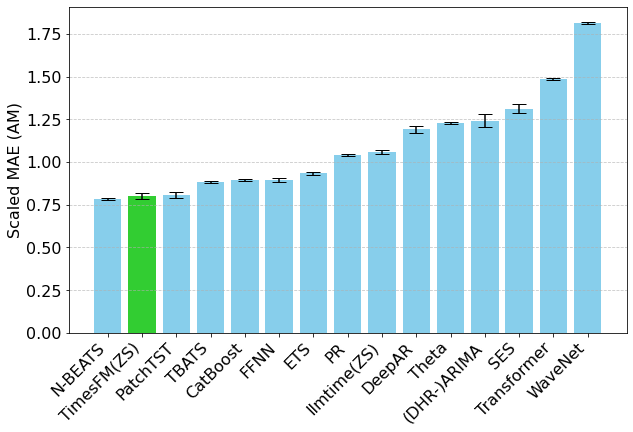
\includegraphics[width=\textwidth]{monash_mae_am.png} % 'placeholder1'을 이미지 파일 이름으로 바꾸세요.
     \caption{\scriptsize{\rev{Monash Archive}~\citep{godahewa2021monash}}}
     \label{fig:monash_mae_am}
  \end{subfigure}
  \hfill % 하위 그림 사이에 약간의 공백을 추가합니다.
  \begin{subfigure}[b]{0.3\textwidth}
     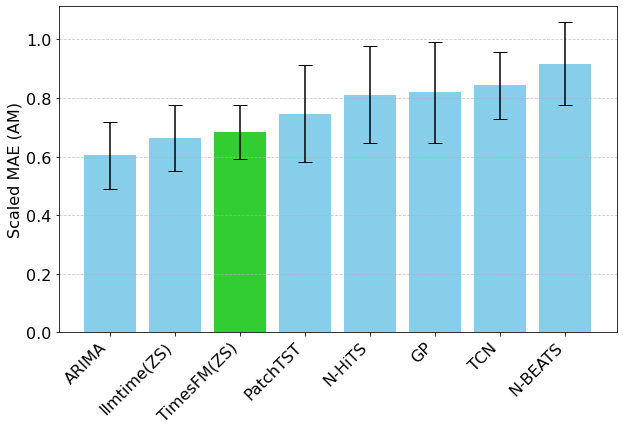
\includegraphics[width=\textwidth]{darts_chart_200m_am_final.png} % 'placeholder2'를 이미지 파일 이름으로 바꾸세요.
     \caption{\scriptsize{\rev{Darts}~\citep{herzen2022darts}}}
     \label{fig:darts_am}
  \end{subfigure}
  \hfill % 하위 그림 사이에 약간의 공백을 추가합니다.
  \begin{subfigure}[b]{0.3\textwidth}
     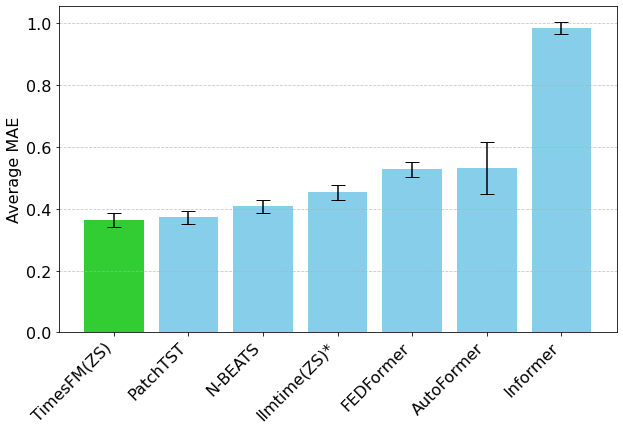
\includegraphics[width=\textwidth]{autoformer_chart_200m_final.png} % 'placeholder3'을 이미지 파일 이름으로 바꾸세요.
     \caption{\scriptsize{ETT (Horizons 96 and 192)~\citep{zhou2021informer}}}
     \label{fig:informer_am}
  \end{subfigure}
\caption{\rev{우리는 세 가지 데이터 세트 그룹의 평균 성능을 보고합니다. 모든 수치에서 측정항목이 낮을수록 더 좋고 오류 막대는 하나의 표준 오류를 나타냅니다. 기준선 중에서 \ours~및 llmtime만 제로샷입니다. (a)에서는 Monash 데이터세트에 대한 결과를 보고합니다. \rev{데이터세트의 규모가 다르기 때문에 우리는 순진한 기준선의 MAE에 의해 조정된 산술 평균(AM)을 취합니다.} \ours~은 톱모델 엔비츠(N-BEATS)의 의미 속에 있음을 알 수 있습니다. (b)에서는 Darts 벤치마크에서 유사한 규모의 MAE를 보고합니다. \ours~는 이 경우 ARIMA인 메서드의 최상위에 해당합니다. 이러한 데이터 세트에는 각각 하나의 시계열이 있으므로 통계 방법은 딥 러닝 방법과 경쟁력이 있습니다. 마지막으로 (c)에서는 4개 ETT 데이터 세트, 즉 총 8개 작업에 대한 96개 및 192개 지평선 예측 작업에 대한 평균 MAE를 보고합니다. \ours~및 PatchTST는 이 경우 가장 성능이 좋은 모델입니다.}}
  \label{fig:all_bar_charts_am}
\end{figure*}

\subsubsection{Darts}
\label{app:darts}
Table~\ref{tab:darts}의 8개 데이터세트 모두에서 개별적으로 MAE 결과를 제시합니다. \ours~은 명확한 계절 패턴이 있는 모든 데이터세트에서 좋은 성능을 보이는 것을 볼 수 있습니다. 평균적으로 우리는 최고의 모델의 상당한 수준 내에 있습니다. Darts에는 전체적으로 8개의 시계열만 있으므로 이러한 평가의 신뢰 구간은 매우 넓습니다.

그림~\ref{fig:darts_all_4x4}에서는 예측과 일부 기준선을 시각적으로 비교합니다.
\begin{table}[!ht]
\centering
\caption{Darts 데이터세트용 MAE. 또한 컨텍스트의 마지막 값을 반복적으로 예측하는 순진한 기준선도 포함합니다.}
\label{tab:darts}
\resizebox{\textwidth}{!}{
\begin{tabular}{lrrrrrrrrr}
\toprule
 & GP & ARIMA & TCN & N-BEATS & N-HiTS & llmtime(ZS) & \ours(ZS) & \rev{패치TST} & NAIVE \\
\midrule
AirPassengersDataset & 34.67 & 24.03 & 54.96 & 97.89 & 59.16 & 34.37 & \rev{62.51} & \rev{44.65} & 81.45 \\
AusBeerDataset & 102.05 & 17.13 & 30.90 & 10.39 & 34.23 & 16.13 & \rev{11.94} & \rev{21.97} & 96.35 \\
GasRateCO2Dataset & 2.27 & 2.37 & 2.64 & 2.63 & 3.85 & 3.50 & \rev{2.50} & \rev{2.67} & 2.29 \\
MonthlyMilkDataset & 30.33 & 37.19 & 70.86 & 33.64 & 32.73 & 9.68 & \rev{28.09} & \rev{42.60} & 85.71 \\
SunspotsDataset & 53.74 & 43.56 & 51.82 & 73.15 & 49.93 & 47.34 & \rev{41.40} & \rev{62.33} & 48.24 \\
WineDataset & 4552.06 & 2306.70 & 3287.14 & 4562.02 & 3909.51 & 1569.32 & \rev{2871.33} & \rev{2498.69} & 4075.28 \\
WoolyDataset & 649.98 & 588.78 & 1158.79 & 903.01 & 382.09 & 808.73 & \rev{728.92} & \rev{542.28}  & 1210.33 \\
HeartRateDataset & 5.65 & 5.56 & 5.49 & 6.57 & 6.10 & 6.21 & \rev{5.85} & \rev{6.74} & 5.92 \\
\midrule
스케일링된 MAE(산술 평균) & 0.8193 & 0.6045 & 0.8427 & 0.9176 & 0.8109 & 0.6641 & 0.6829 & \rev{0.7462} &1.0000 \\
스케일링된 MAE(기하 평균) & 0.7509 & 0.5219 & 0.7946 & 0.7316 & 0.6936 & 0.4882 & 0.5767 & \rev{0.6458} &1.0000 \\
\bottomrule
\end{tabular}
}
\end{table}


\subsubsection{Monash}
\label{app:monash}

\begin{table}[!ht]
\centering
\caption{우리는 Monash 기준선 크기에 따라 방법에 대한 평균 MAE 결과를 제시합니다. 또한 컨텍스트의 마지막 값을 반복적으로 예측하는 순진한 기준선도 포함합니다.}
\label{tab:monash_mae}
\resizebox{1\textwidth}{!}{
\begin{tabular}{lrrrrrrrrrrrrrrrr}
\toprule
 & llmtime(ZS) & SES & Theta & TBATS & ETS & (DHR-)ARIMA & PR & CatBoost & FFNN & DeepAR & N-BEATS & WaveNet & Transformer & \rev{패치TST(ZS)} & \ours(ZS) &  NAIVE \\
Dataset &  &  &  &  &  &  &  &  &  &  &  &  &  &  &  &  \\
\midrule
호주의 전력 수요 & 459.96 & 659.60 & 665.04 & 370.74 & 1282.99 & 1045.92 & 247.18 & 241.77 & 258.76 & 302.41 & 213.83 & 227.50 & 231.45 & \rev{382.23} & \rev{448.81} & 659.60 \\
bitcoin & 1.75e18 & 5.33e18 & 5.33e18 & 9.90e17 & 1.10e18 & 3.62e18 & 6.66e17 & 1.93e18 & 1.45e18 & 1.95e18 & 1.06e18 & 2.46e18 & 2.61e18 & \rev{1.11e18} & \rev{1.3e18} & \rev{7.77e17} \\
보행자 수 & 70.20 & 170.87 & 170.94 & 222.38 & 216.50 & 635.16 & 44.18 & 43.41 & 46.41 & 44.78 & 66.84 & 46.46 & 47.29 & \rev{51.27} & \rev{40.71} & 170.88 \\
weather & 2.32 & 2.24 & 2.51 & 2.30 & 2.35 & 2.45 & 8.17 & 2.51 & 2.09 & 2.02 & 2.34 & 2.29 & 2.03 & \rev{2.07} & \rev{2.07} & 2.36 \\
매일 nn5 & 9.39 & 6.63 & 3.80 & 3.70 & 3.72 & 4.41 & 5.47 & 4.22 & 4.06 & 3.94 & 4.92 & 3.97 & 4.16 & \rev{3.77} & \rev{3.54} & 8.26 \\
매주 nn5 & 15.91 & 15.66 & 15.30 & 14.98 & 15.70 & 15.38 & 14.94 & 15.29 & 15.02 & 14.69 & 14.19 & 19.34 & 20.34 & \rev{17.00} & \rev{14.67} & 16.71 \\
연간 관광 & 140081.78 & 95579.23 & 90653.60 & 94121.08 & 94818.89 & 95033.24 & 82682.97 & 79567.22 & 79593.22 & 71471.29 & 70951.80 & 69905.47 & 74316.52 & \rev{224411.89} & \rev{109977.29} & 99456.05 \\
분기별 관광 & 14121.09 & 15014.19 & 7656.49 & 9972.42 & 8925.52 & 10475.47 & 9092.58 & 10267.97 & 8981.04 & 9511.37 & 8640.56 & 9137.12 & 9521.67 & \rev{21276.98} &  \rev{12102.04} & 15845.10 \\
월간 관광 & 4724.94 & 5302.10 & 2069.96 & 2940.08 & 2004.51 & 2536.77 & 2187.28 & 2537.04 & 2022.21 & 1871.69 & 2003.02 & 2095.13 & 2146.98 & \rev{4596.21} & \rev{3183.77} & 5636.83 \\
CIF 2016 & 715086.33 & 581875.97 & 714818.58 & 855578.40 & 642421.42 & 469059.49 & 563205.57 & 603551.30 & 1495923.44 & 3200418.00 & 679034.80 & 5998224.62 & 4057973.04 & \rev{8374813.14} & \rev{773980.44} & 386526.37 \\
코로나 사망 & 304.68 & 353.71 & 321.32 & 96.29 & 85.59 & 85.77 & 347.98 & 475.15 & 144.14 & 201.98 & 158.81 & 1049.48 & 408.66 & \rev{348.60} & \rev{209.80} & \rev{353.71} \\
프레드 MD & 2013.49 & 2798.22 & 3492.84 & 1989.97 & 2041.42 & 2957.11 & 8921.94 & 2475.68 & 2339.57 & 4264.36 & 2557.80 & 2508.40 & 4666.04 & \rev{4965.51} & \rev{947.12} & 2825.67 \\
시간당 교통량 & 0.03 & 0.03 & 0.03 & 0.04 & 0.03 & 0.04 & 0.02 & 0.02 & 0.01 & 0.01 & 0.02 & 0.02 & 0.01 & \rev{0.01} & \rev{0.01} & 0.03 \\
주간 교통량 & 1.17 & 1.12 & 1.13 & 1.17 & 1.14 & 1.22 & 1.13 & 1.17 & 1.15 & 1.18 & 1.11 & 1.20 & 1.42 & \rev{1.23} & \rev{1.12} & 1.19 \\
saugeenday & 28.63 & 21.50 & 21.49 & 22.26 & 30.69 & 22.38 & 25.24 & 21.28 & 22.98 & 23.51 & 27.92 & 22.17 & 28.06 & \rev{22.33} & \rev{24.6}3 & 21.50 \\
우리 탄생 & 459.43 & 1192.20 & 586.93 & 399.00 & 419.73 & 526.33 & 574.93 & 441.70 & 557.87 & 424.93 & 422.00 & 504.40 & 452.87 & \rev{1193.28} & \rev{437.27} & 1152.67 \\
hospital & 24.62 & 21.76 & 18.54 & 17.43 & 17.97 & 19.60 & 19.24 & 19.17 & 22.86 & 18.25 & 20.18 & 19.35 & 36.19 & \rev{20.87} & \rev{19.41} & 24.07 \\
태양 주간 & 2049.09 & 1202.39 & 1210.83 & 908.65 & 1131.01 & 839.88 & 1044.98 & 1513.49 & 1050.84 & 721.59 & 1172.64 & 1996.89 & 576.35 & \rev{1093.46} & \rev{1258.27} & 1729.41 \\
\midrule
스케일링된 MAE(산술 평균) & 1.0588 & 1.3115 & 1.2295 & 0.8824 & 0.9337 & 1.2427 & 1.0382 & 0.8924 & 0.8942 & 1.1925 & 0.7844 & 1.8119 & 1.4840 & 2.1419 & 0.8005 & 1.0000 \\
스케일링된 MAE(기하 평균) & 0.9715 & 1.0855 & 0.9371 & 0.7736 & 0.8104 & 0.9449 & 0.8218 & 0.7733 & 0.7044 & 0.7477 & 0.7005 & 0.9384 & 0.8619 & 1.0557 & 0.6846 & 1.0000 \\
\bottomrule
\end{tabular}
}



\end{table}

% \begin{table}[!ht]
% \centering
% \caption{We present the mean msMAPE results for our methods along size monash baselines. We also include the naive baseline that predicts the last values in the context repeatedly.}
% \label{tab:monash_msmape}
% \resizebox{\textwidth}{!}{
% \begin{tabular}{lrrrrrrrrrrrrrrr}
% \toprule
%  & llmtime(ZS) & SES & Theta & TBATS & ETS & (DHR-)ARIMA & PR & CatBoost & FFNN & DeepAR & N-BEATS & WaveNet & Transformer & \ours(ZS) & NAIVE \\
% Dataset &  &  &  &  &  &  &  &  &  &  &  &  &  &  &  \\
% \midrule
% australian electricity demand & 15.30 & 22.07 & 22.18 & 13.70 & 44.22 & 28.75 & 8.76 & 8.35 & 9.22 & 12.77 & 7.74 & 8.07 & 8.68 & 17.27 & 22.07 \\
% bitcoin & 22.70 & 30.31 & 40.36 & 20.12 & 20.65 & 31.11 & 21.48 & 29.78 & 21.00 & 21.16 & 31.95 & 22.16 & 23.32 & 42.00 & 192.46 \\
% pedestrian counts & 53.02 & 121.39 & 122.08 & 119.76 & 148.48 & 138.58 & 40.29 & 45.54 & 39.30 & 36.10 & 54.15 & 34.22 & 36.16 & 50.73 & 121.35 \\
% weather & 34.05 & 50.85 & 56.19 & 58.06 & 51.47 & 57.98 & 106.01 & 59.12 & 38.17 & 36.46 & 50.87 & 40.13 & 35.35 & 50.85 & 36.81 \\
% nn5 daily & 47.43 & 35.38 & 21.93 & 21.11 & 21.49 & 25.91 & 30.20 & 24.04 & 23.30 & 23.75 & 28.47 & 22.65 & 23.18 & 23.46 & 48.09 \\
% nn5 weekly & 12.28 & 12.24 & 11.96 & 11.62 & 12.29 & 11.83 & 11.45 & 11.67 & 11.49 & 11.52 & 10.93 & 14.95 & 14.83 & 11.01 & 13.26 \\
% tourism yearly & 48.28 & 34.10 & 31.93 & 33.94 & 36.52 & 33.39 & 46.92 & 31.54 & 33.73 & 34.06 & 30.24 & 28.80 & 34.66 & 30.14 & 42.14 \\
% tourism quarterly & 25.25 & 27.41 & 15.37 & 17.16 & 15.07 & 16.58 & 15.86 & 16.53 & 16.20 & 15.29 & 14.45 & 15.56 & 16.97 & 19.92 & 31.68 \\
% tourism monthly & 33.53 & 36.39 & 19.89 & 21.20 & 19.02 & 19.73 & 21.11 & 21.10 & 20.11 & 18.35 & 20.42 & 18.92 & 19.74 & 22.77 & 40.40 \\
% cif 2016 & 18.63 & 14.94 & 13.04 & 12.19 & 12.18 & 11.69 & 12.32 & 14.86 & 12.31 & 13.54 & 11.71 & 18.82 & 12.55 & 20.00 & 15.41 \\
% covid deaths & 20.65 & 15.35 & 15.57 & 8.71 & 8.64 & 9.26 & 18.34 & 15.40 & 18.58 & 34.18 & 32.36 & 14.50 & 40.71 & 15.89 & 134.79 \\
% fred md & 9.75 & 8.72 & 9.72 & 7.97 & 8.40 & 7.98 & 30.77 & 9.16 & 8.99 & 8.33 & 8.32 & 9.08 & 11.26 & 8.47 & 8.76 \\
% traffic hourly & 11.70 & 8.73 & 8.73 & 12.58 & 9.84 & 11.72 & 5.97 & 7.94 & 4.30 & 4.16 & 5.16 & 5.22 & 4.10 & 4.76 & 8.73 \\
% traffic weekly & 12.85 & 12.40 & 12.48 & 12.80 & 12.63 & 13.45 & 12.46 & 12.90 & 12.64 & 13.13 & 12.31 & 13.21 & 15.18 & 12.48 & 12.98 \\
% saugeenday & 58.53 & 35.99 & 35.97 & 37.34 & 67.50 & 37.55 & 45.32 & 35.55 & 39.32 & 40.22 & 56.03 & 37.02 & 56.62 & 43.31 & 35.99 \\
% us births & 4.48 & 11.77 & 5.82 & 3.81 & 4.05 & 5.17 & 5.75 & 4.23 & 5.55 & 4.13 & 4.17 & 4.88 & 4.36 & 3.94 & 11.35 \\
% hospital & 21.68 & 17.94 & 17.27 & 17.55 & 17.46 & 17.79 & 17.56 & 18.04 & 18.29 & 17.41 & 17.72 & 17.51 & 20.04 & 17.86 & 21.55 \\
% solar weekly & 37.33 & 24.59 & 24.76 & 19.05 & 22.93 & 17.87 & 21.65 & 29.35 & 21.52 & 15.00 & 24.05 & 32.50 & 12.26 & 24.20 & 32.80 \\
% \bottomrule
% \end{tabular}
% }
% \end{table}

Table~\ref{tab:monash_mae}에는 주요 Figure~\ref{fig:monash_mae} 뒤에 있는 실제 MAE 번호가 표시됩니다. Figure~\ref{fig:monash_4x4}에서는 제로샷 예측의 몇 가지 예를 제시합니다. 대부분의 데이터세트의 경우 컨텍스트 창을 512개로 제한되는 데이터세트의 계열의 최대 길이로 설정합니다(공식 Monash 기준선에서 사용되는 통계 모델과 유사). \rev{일부 데이터세트의 경우 컨텍스트 길이에 대한 추론 시간 조정을 수행했습니다. 즉, 컨텍스트 길이가 32, 64이고 최대 허용되는 훈련 세트의 마지막 수평선 길이 포인트 수를 예측하고 이 검증 측정 항목과 관련하여 가장 적합한 것을 선택했습니다. 대부분의 Monash DL 기준선은 훈련 중에 다양한 데이터세트에 대해 서로 다른 컨텍스트 길이를 사용하고 우리 모델은 완전히 제로샷이기 때문에 이것은 공평합니다. 이러한 데이터세트에 사용된 최대 컨텍스트 길이는 (cif 2016, 32), (연간 관광, 32), (covid 사망, 32), (비트코인, 32), (월간 관광, 32) 및 (월간 관광, 64)}입니다.


\subsubsection{Informer}
\label{app:informer}
Table~\ref{tab:inf}에서 고려된 수평선 쌍인 모든 데이터 세트에 대한 테스트 세트의 마지막 분할에 MAE를 제시합니다. llmtime에 대한 값비싼 평가로 인해 ~\citep{gruver2023large}에서와 같이 원래 테스트 분할의 마지막 테스트 창에 결과가 보고됩니다.


\begin{table}[!ht]
\centering
\caption{예측 범위 96 및 192에 대한 ETT 데이터 세트에 대한 MAE. llmtime에 대한 값비싼 평가로 인해 결과는 원래 테스트 분할의 마지막 테스트 창에 보고됩니다.}
\label{tab:inf}
\resizebox{1\textwidth}{!}{
\begin{tabular}{lrrrrrrr}
\toprule
& lm시간(ZS)* & PatchTST & \rev{패치TST(ZS)} & FEDFormer & AutoFormer & Informer  & TimesFM(ZS) \\
Dataset &  &  &  &  &  &  & \\
\midrule
ETTh1(수평=96)   & 0.42 & 0.41 & \rev{0.39} & 0.58 & 0.55 & 0.76 & \rev{0.45} \\
ETTh1(수평=192)  & 0.50 & 0.49 & \rev{0.50} & 0.64 & 0.64 & 0.78 & \rev{0.53} \\
ETTh2(수평=96)   & 0.33 & 0.28 & \rev{0.37} & 0.67 & 0.65 & 1.94 & \rev{0.35} \\
ETTh2(수평=192)  & 0.70 & 0.68 & \rev{0.59} & 0.82 & 0.82 & 2.02 & \rev{0.62} \\
ETTm1(수평=96)   & 0.37 & 0.33 & \rev{0.24} & 0.41 & 0.54 & 0.71 & \rev{0.19} \\
ETTm1(수평=192)  & 0.71 & 0.31 & \rev{0.26} & 0.49 & 0.46 & 0.68 & \rev{0.26} \\
ETTm2(수평=96)   & 0.29 & 0.23 & \rev{0.22} & 0.36 & 0.29 & 0.48 & \rev{0.24} \\
ETTm2(수평=192)  & 0.31 & 0.25 & \rev{0.22} & 0.25 & 0.30 & 0.51 & \rev{0.27} \\
\midrule
Avg                  & 0.45 & 0.37 & 0.35        & 0.53 & 0.53 & 0.99 & 0.36 \\ 
\bottomrule
\end{tabular}
}
\end{table}

% \begin{table}[!ht]
% \centering
% \caption{MAE for ETT datasets for prediction horizons 96 and 192. Owing to expensive evaluations for llmtime, the results are reported on the last test window of the original test split.}
% \label{tab:inf_alt}
% \begin{tabular}{lrrrrrr}
% \toprule
%  & llmtime(ZS) & PatchTST & \ours(ZS) & FEDFormer & AutoFormer & Informer \\
% Dataset &  &  &  &  &  &  \\
% \midrule
% ETTh1 (Horizon=96) & 0.42 & 0.41 & 0.37 & 0.58 & 0.55 & 0.76 \\
% ETTh1 (Horizon=192) & 0.50 & 0.49 & 0.49 & 0.64 & 0.64 & 0.78 \\
% ETTh2 (Horizon=96) & 0.33 & 0.28 & 0.28 & 0.67 & 0.65 & 1.94 \\
% ETTh2 (Horizon=192) & 0.70 & 0.68 & 0.58 & 0.82 & 0.82 & 2.02 \\
% ETTm1 (Horizon=96) & 0.37 & 0.33 & 0.25 & 0.41 & 0.54 & 0.71 \\
% ETTm1 (Horizon=192) & 0.71 & 0.31 & 0.24 & 0.49 & 0.46 & 0.68 \\
% ETTm2 (Horizon=96) & 0.29 & 0.23 & 0.28 & 0.36 & 0.29 & 0.48 \\
% ETTm2 (Horizon=192) & 0.31 & 0.25 & 0.24 & 0.25 & 0.30 & 0.51 \\
% \bottomrule
% \end{tabular}
% \end{table}
\subsection{모델에 대한 추가 세부 사항}
\label{app:moremodels}
이제 \ours~및 기타 기준에 대한 구현 세부 정보를 제공합니다.

{\bf \ours.} 주요 200M 모델의 경우 주의 헤드 16개, 레이어 20개, 입력 패치 길이 32, 출력 패치 길이 128을 사용합니다. 모델 차원은 1280으로 설정됩니다. 최대 학습 속도 $5e-4$의 레이어 표준과 코사인 붕괴 학습 속도 일정으로 훈련합니다. 다양한 크기에 대한 \ours~의 하이퍼파라미터는 Table~\ref{tab:hparams}에 나와 있습니다. 설정은 절제 모델이 아닌 기본 모델에 대한 것입니다. 변환기 레이어의 잔여 블록과 FFN의 숨겨진 희미함은 모델 치수와 동일하게 설정됩니다. 변환기 레이어에서는 레이어 규범을 유지하지만 잔차 블록에서는 유지하지 않습니다.

\begin{table}[!ht]
\centering
\caption{\ours의 초매개변수}
\label{tab:hparams}
\begin{tabular}{lrrrrrr}
\toprule
 & num\textunderscore 레이어 & 모델\textunderscore 어두워짐 & 출력\textunderscore 패치\textunderscore 렌& 입력\textunderscore 패치\textunderscore 렌 & num\textunderscore 헤드 & dropout \\
Size &  &  &  &  &  &  \\
\midrule
200M  & 20 & 1280 & 128 & 32 & 16 & 0.2 \\
70M  & 10 & 1024 & 128 & 32 & 16 & 0.2 \\
17M  & 10 & 512 & 128 & 32 & 16 & 0.2 \\
\bottomrule
\end{tabular}
\end{table}

{\bf Monash 기준선.} Monash 기준선에 대한 원시 측정항목은 원본 논문 보충 자료의 표 9 및 11에서 직접 가져왔습니다~\citep{godahewa2021monash}. llmtime의 경우 ~\citep{gruver2023large} 작성자가 제공한 미리 계산된 출력을 사용합니다.

{\bf Darts 기준선.} 모든 Darts 기준선에 대해 ~\citep{gruver2023large} 작성자가 제공한 미리 계산된 출력을 사용합니다. 자세한 내용은 해당 문서의 섹션 C.1을 참조하세요.


{\bf Informer Baselines.} FEDFormer~\citep{zhou2022fedformer}, Autoformer~\citep{wu2021autoformer}, Informer~\citep{zhou2021informer} 및 PatchTST~\citep{nie2022time}의 경우 원래 하이퍼 매개변수와 구현을 사용합니다. 본 논문에 제시된 결과는 llmtime~\citep{gruver2023large} 논문에 명시된 대로 length horizon length의 마지막 테스트 창에서 얻은 것입니다.

저자~\footnote{\url{https://github.com/ngruver/llmtime/blob/main/experiments/run_monash.py}}가 제공했지만 ETT 데이터세트에 맞게 조정된 코드를 사용하여 llmtime 예측을 생성합니다. 2024년 1월부터 OpenAI는 GPT-3에 대한 액세스를 중단했기 때문에 GPT-3.5-Turbo 모델을 사용해야 했습니다.


\subsection{날짜 특징}
\label{app:date_features}
앞서 언급했듯이 사전 훈련된 단일 모델을 구축하고 있으므로 훈련 시간 동안 데이터 세트 특정 동적 또는 정적 공변량을 가질 수 없습니다. 그러나 날짜/시간 열은 모든 시계열 데이터 어디에나 존재하므로 기술적으로 요일, 월 등과 같은 날짜 파생 기능을 $\*x_{t} \in \-R^{r}$로 표시되는 각 시점 $t$에서 벡터로 처리할 수 있습니다.

그렇다면 학습 과제는 다음과 같이 다시 작성될 수 있습니다.
\begin{equation*}
     f: \left( \*y_{1:L}, \*x_{1:L+H} \right) \longrightarrow \hat{\*y}_{L+1:L+H}.
\end{equation*}

이러한 기능을 모델에 통합하는 방법에는 여러 가지가 있습니다. 그 중 하나는 각 패치의 시점 이후에 기능을 직접 연결하는 것입니다. 이 논문에서 우리는 일변량 시계열 입력에 초점을 맞추기로 결정하고 향후 이 개선 사항을 조사할 것입니다.

\subsection{합성 데이터}
\label{app:syn}

우리는 전통적인 통계 모델을 사용하여 일반적인 시계열 패턴을 반영하는 합성 데이터를 생성합니다. 네 가지 간단한 시계열 패턴으로 시작합니다.
\begin{itemize}
    \item 조각별 선형 추세(I). 여기서 조각별 선형 구성 요소의 수는 2와 8 사이에서 무작위로 선택됩니다.
    \item ARMA$(p, q)$ (II), 여기서 $1 \leq p, q \leq 8$ 및 해당 계수는 다변량 가우스 또는 균일에서 생성된 다음 정규화됩니다.
    \item 계절 패턴. 특히 우리는 4~\rev{최대 컨텍스트 길이/2} 시점과 시간 지연 사이의 서로 다른 임의 기간의 사인(III) 및 코사인(IV) 파동을 생성합니다.
\end{itemize}

그런 다음 이 네 가지 구성 요소 (I) - (IV)를 무작위로 활성화/비활성화하고 각각 길이 2048의 시계열을 생성한 다음 균일하게 샘플링된 무작위 가중치를 사용하여 이를 합산하여 합성 데이터 세트에서 각 시계열을 생성합니다. 또한 추세 구성 요소가 선택된 횟수의 50\%을 곱셈적으로 추세를 적용하도록 선택합니다.


\subsection{예시 사례}
\label{app:syn_exp}

우리는 \ours이 생성한 예측을 먼저 몇 가지 합성 사례를 대상으로 한 다음 벤치마크 데이터 세트를 대상으로 시각적 검사를 수행합니다.

그림~\ref{fig:viz-syn-4p}에는 4개의 서로 다른 합성 곡선이 표시됩니다. (1) 서로 다른 기간의 5개 사인 곡선의 합, (2) 선형 스케일링된 사인 곡선, (3) 선형 추세가 있는 사인 곡선, (4) 선형 추세가 있는 최소 2개의 사인 곡선. 우리의 결과는 \ours~가 사람이 쉽게 해석할 수 있는 추세와 계절적 구성 요소를 선택하는 반면 ARIMA와 (적지만) llmtime은 일부 인스턴스에서 실패한다는 것을 나타냅니다.

그림~\ref{fig:visualization-4p}에 표시된 대로 \ours~는 묘사된 실제 시계열의 추세와 계절 패턴 모두 내에서 이러한 미묘한 특성을 효과적으로 포착합니다. 예를 들어 Air Passenger 데이터세트에서 \ours~는 추세에 따른 진폭 증가를 올바르게 포착합니다. 이는 이 데이터세트에서 최고의 MAE를 달성한다는 사실에도 반영됩니다(표~\ref{tab:darts} 참조). 왼쪽의 시간별 교통량 예에서는 \ours~가 컨텍스트에 이상값이 있는 경우에도 계절별 최고치를 정확하게 식별할 수 있는 반면 llmtime은 제외되는 것을 볼 수 있습니다.

\begin{figure}[!ht]
    \centering
    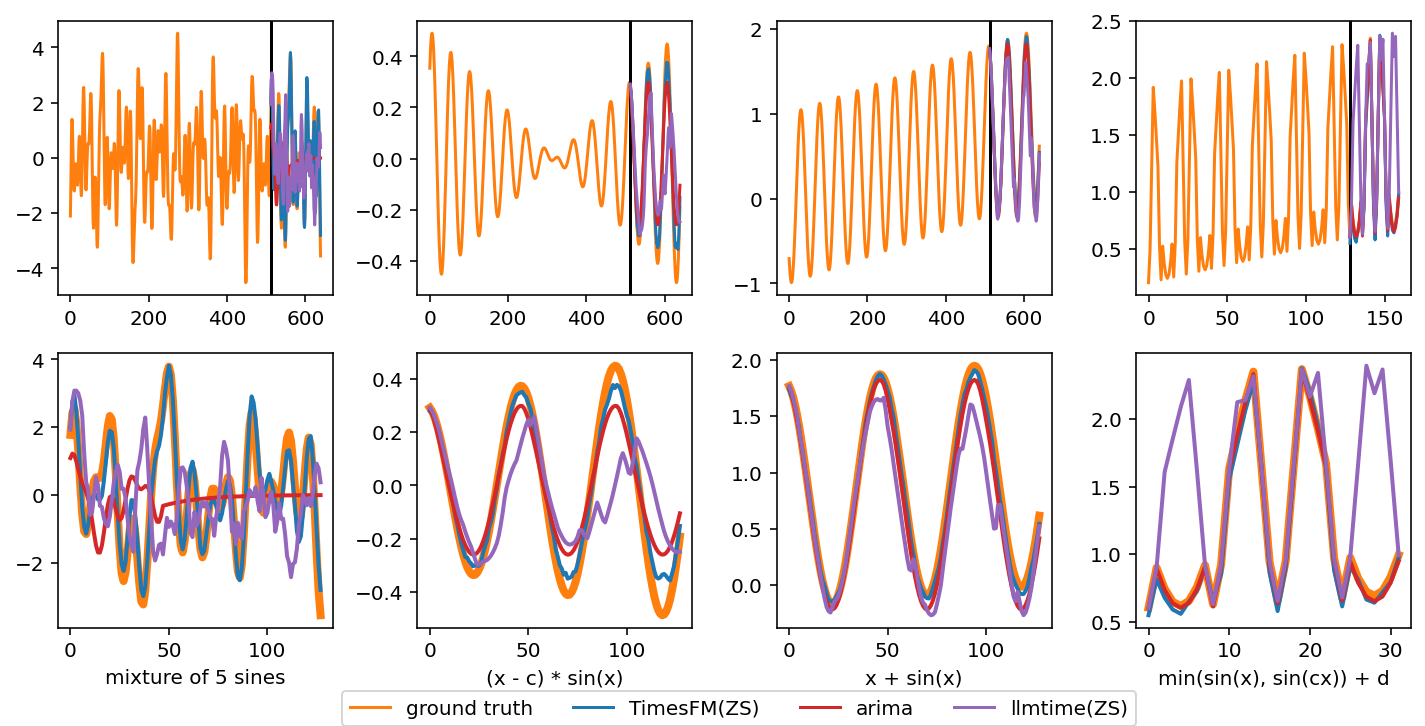
\includegraphics[width=1.0\linewidth]{syn_4.png}
\caption{합성 곡선으로 시각화된 예측. 맨 아래 행은 명확성을 위해 예측 범위를 확대한 것입니다.}
\label{fig:viz-syn-4p}
\end{figure}

\begin{figure}[!ht]
    \centering
    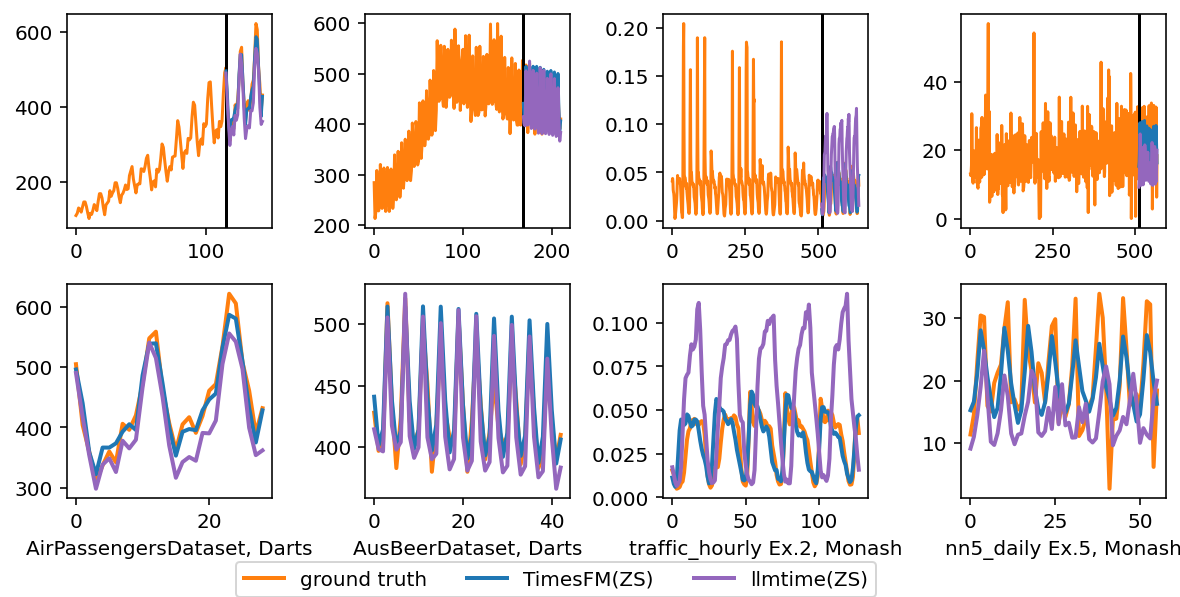
\includegraphics[width=1.0\linewidth]{visualization-4p-darts-monash.png}
\caption{Darts 및 Monash에서 시각화된 예측. 맨 아래 행은 명확성을 위해 예측 범위를 확대한 것입니다.}
\label{fig:visualization-4p}
\end{figure}

Figure~\ref{fig:syn_4x4}, Figure~\ref{fig:darts_all_4x4} 및 Figure~\ref{fig:monash_4x4}에서 더 많은 시각화를 제공합니다.

\begin{figure}[!ht]
\centering
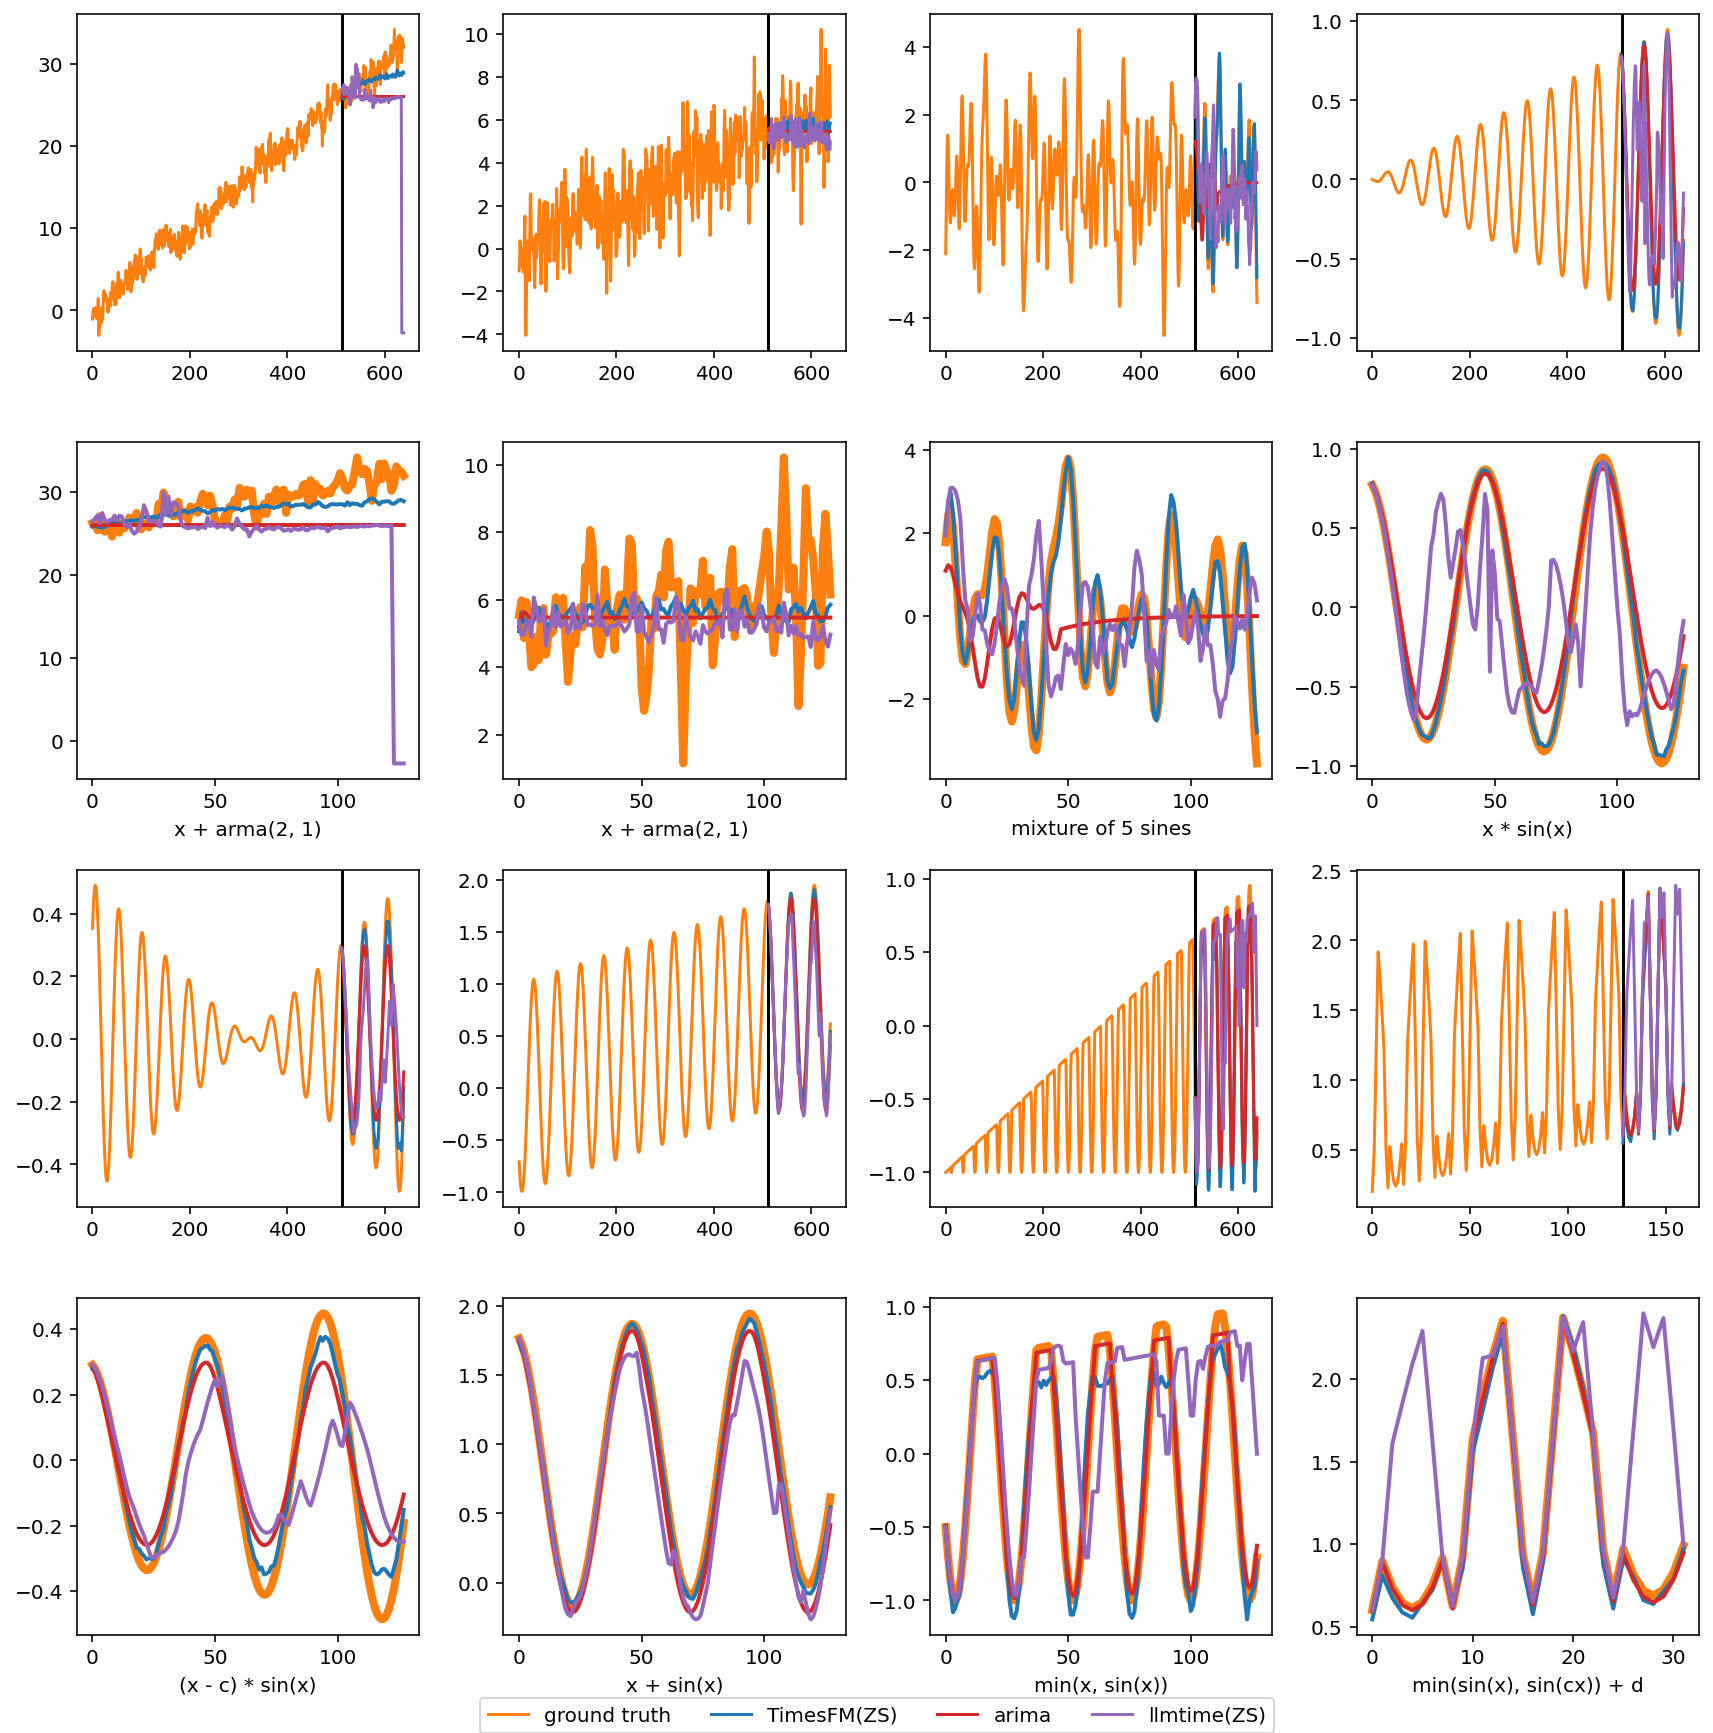
\includegraphics[width=\linewidth]{syn_4x4.png}
\caption{합성 곡선으로 시각화된 예측. 두 번째 행은 명확성을 위해 예측 범위를 확대하여 표시합니다.}
\label{fig:syn_4x4}
\end{figure}

\begin{figure}[!ht]
\centering
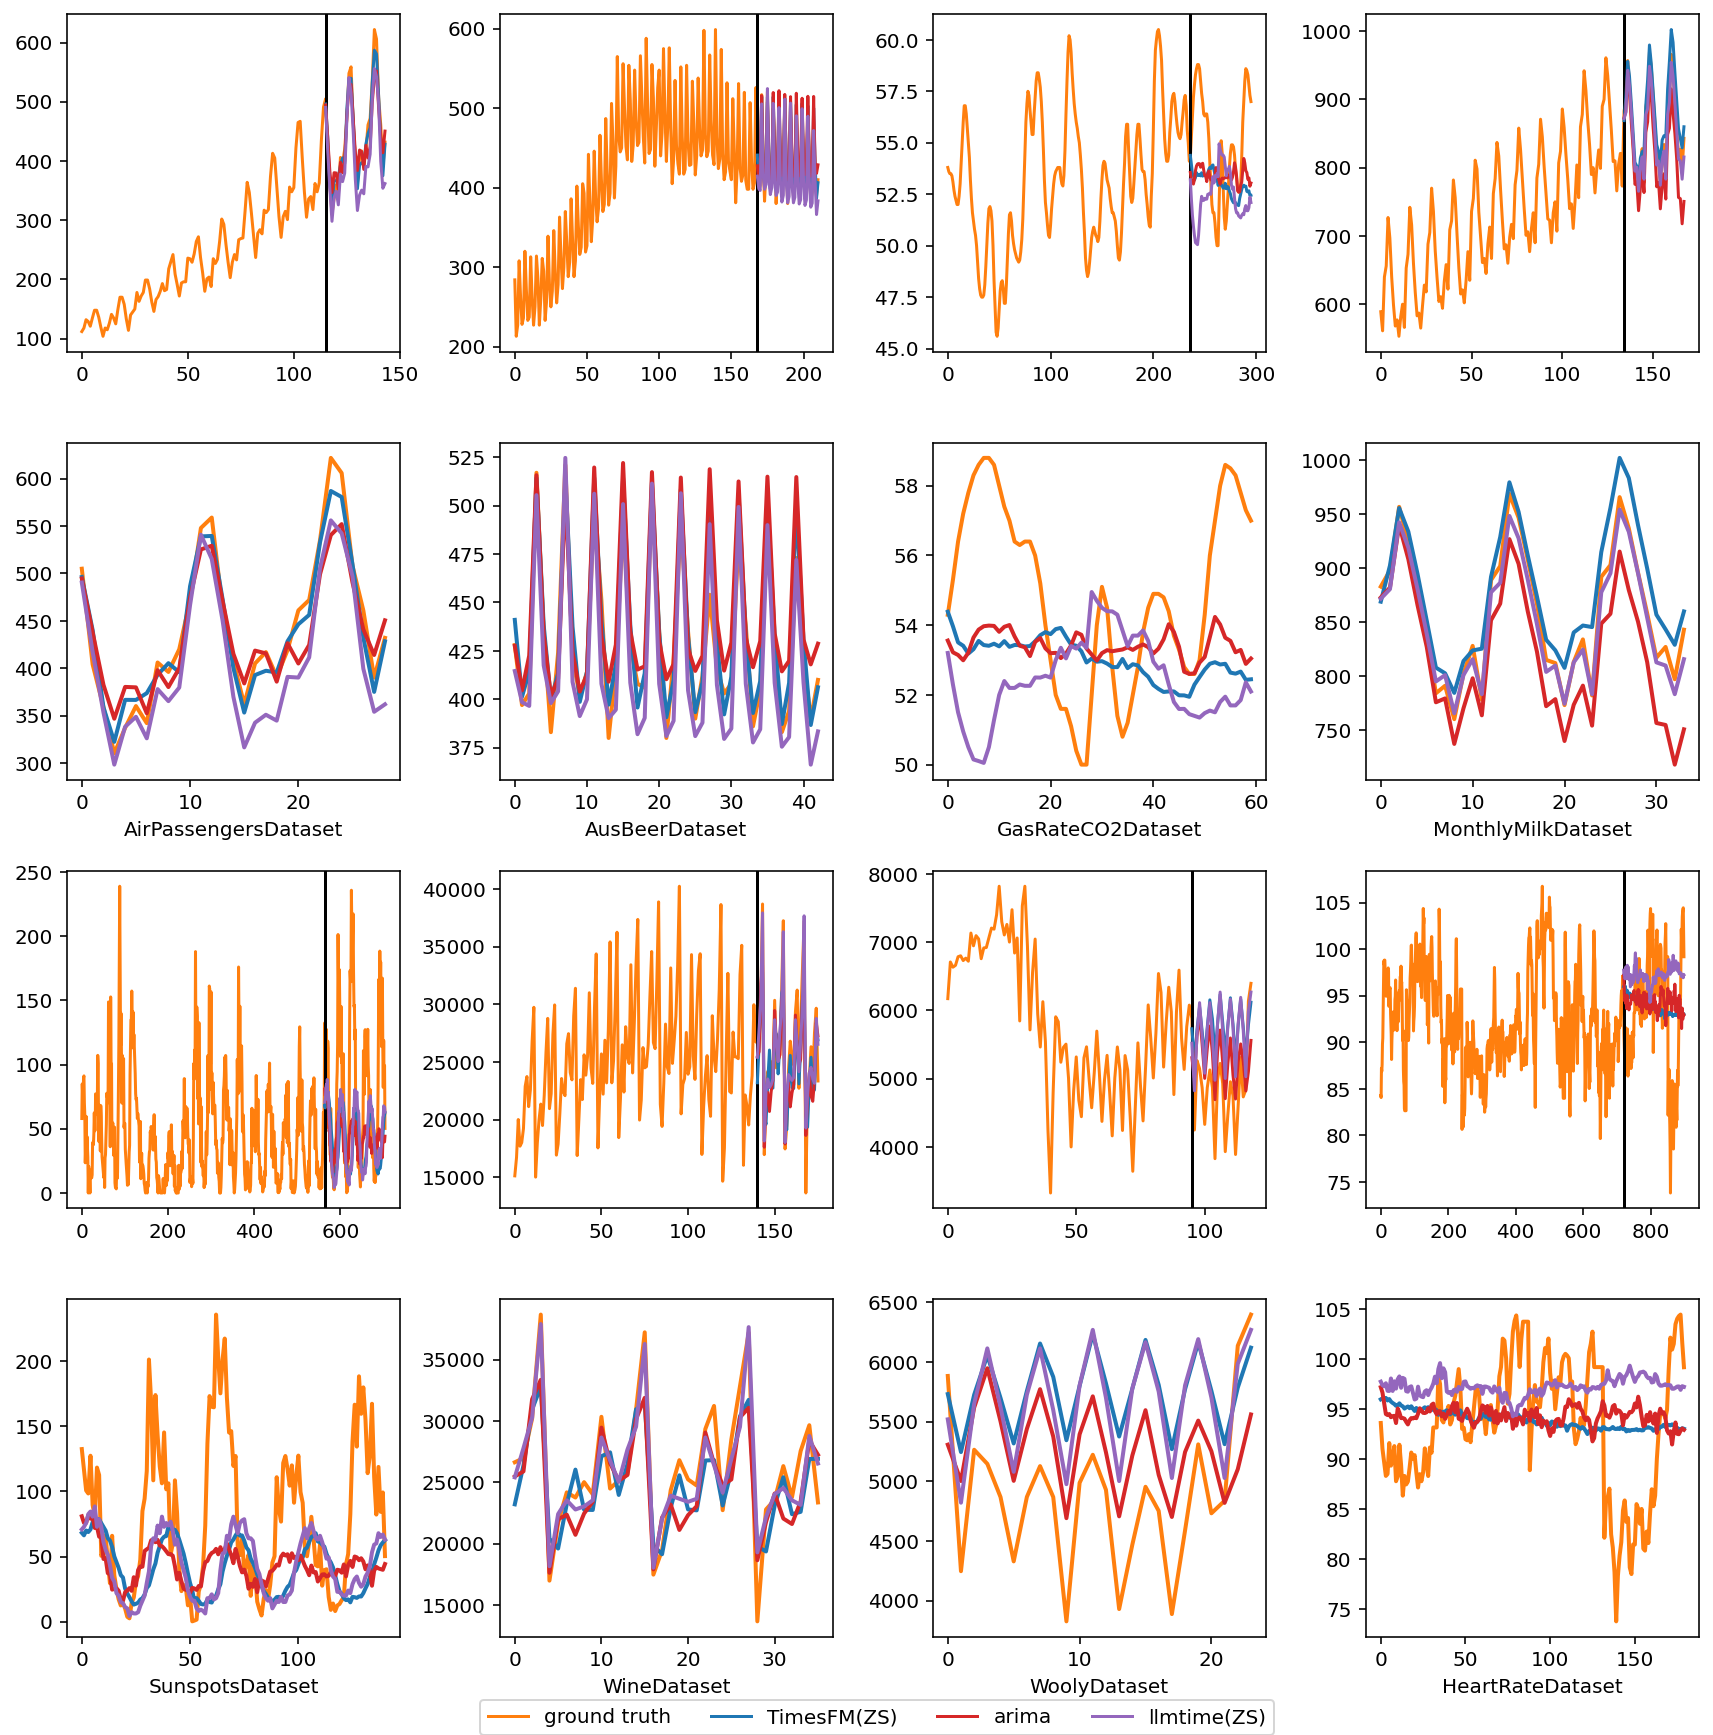
\includegraphics[width=\linewidth]{darts_all_4x4.png}
\caption{모든 Darts 데이터세트에서 시각화된 예측입니다. 두 번째 행은 명확성을 위해 예측 범위를 확대하여 표시합니다.}
\label{fig:darts_all_4x4}
\end{figure}

\begin{figure}[!ht]
\centering
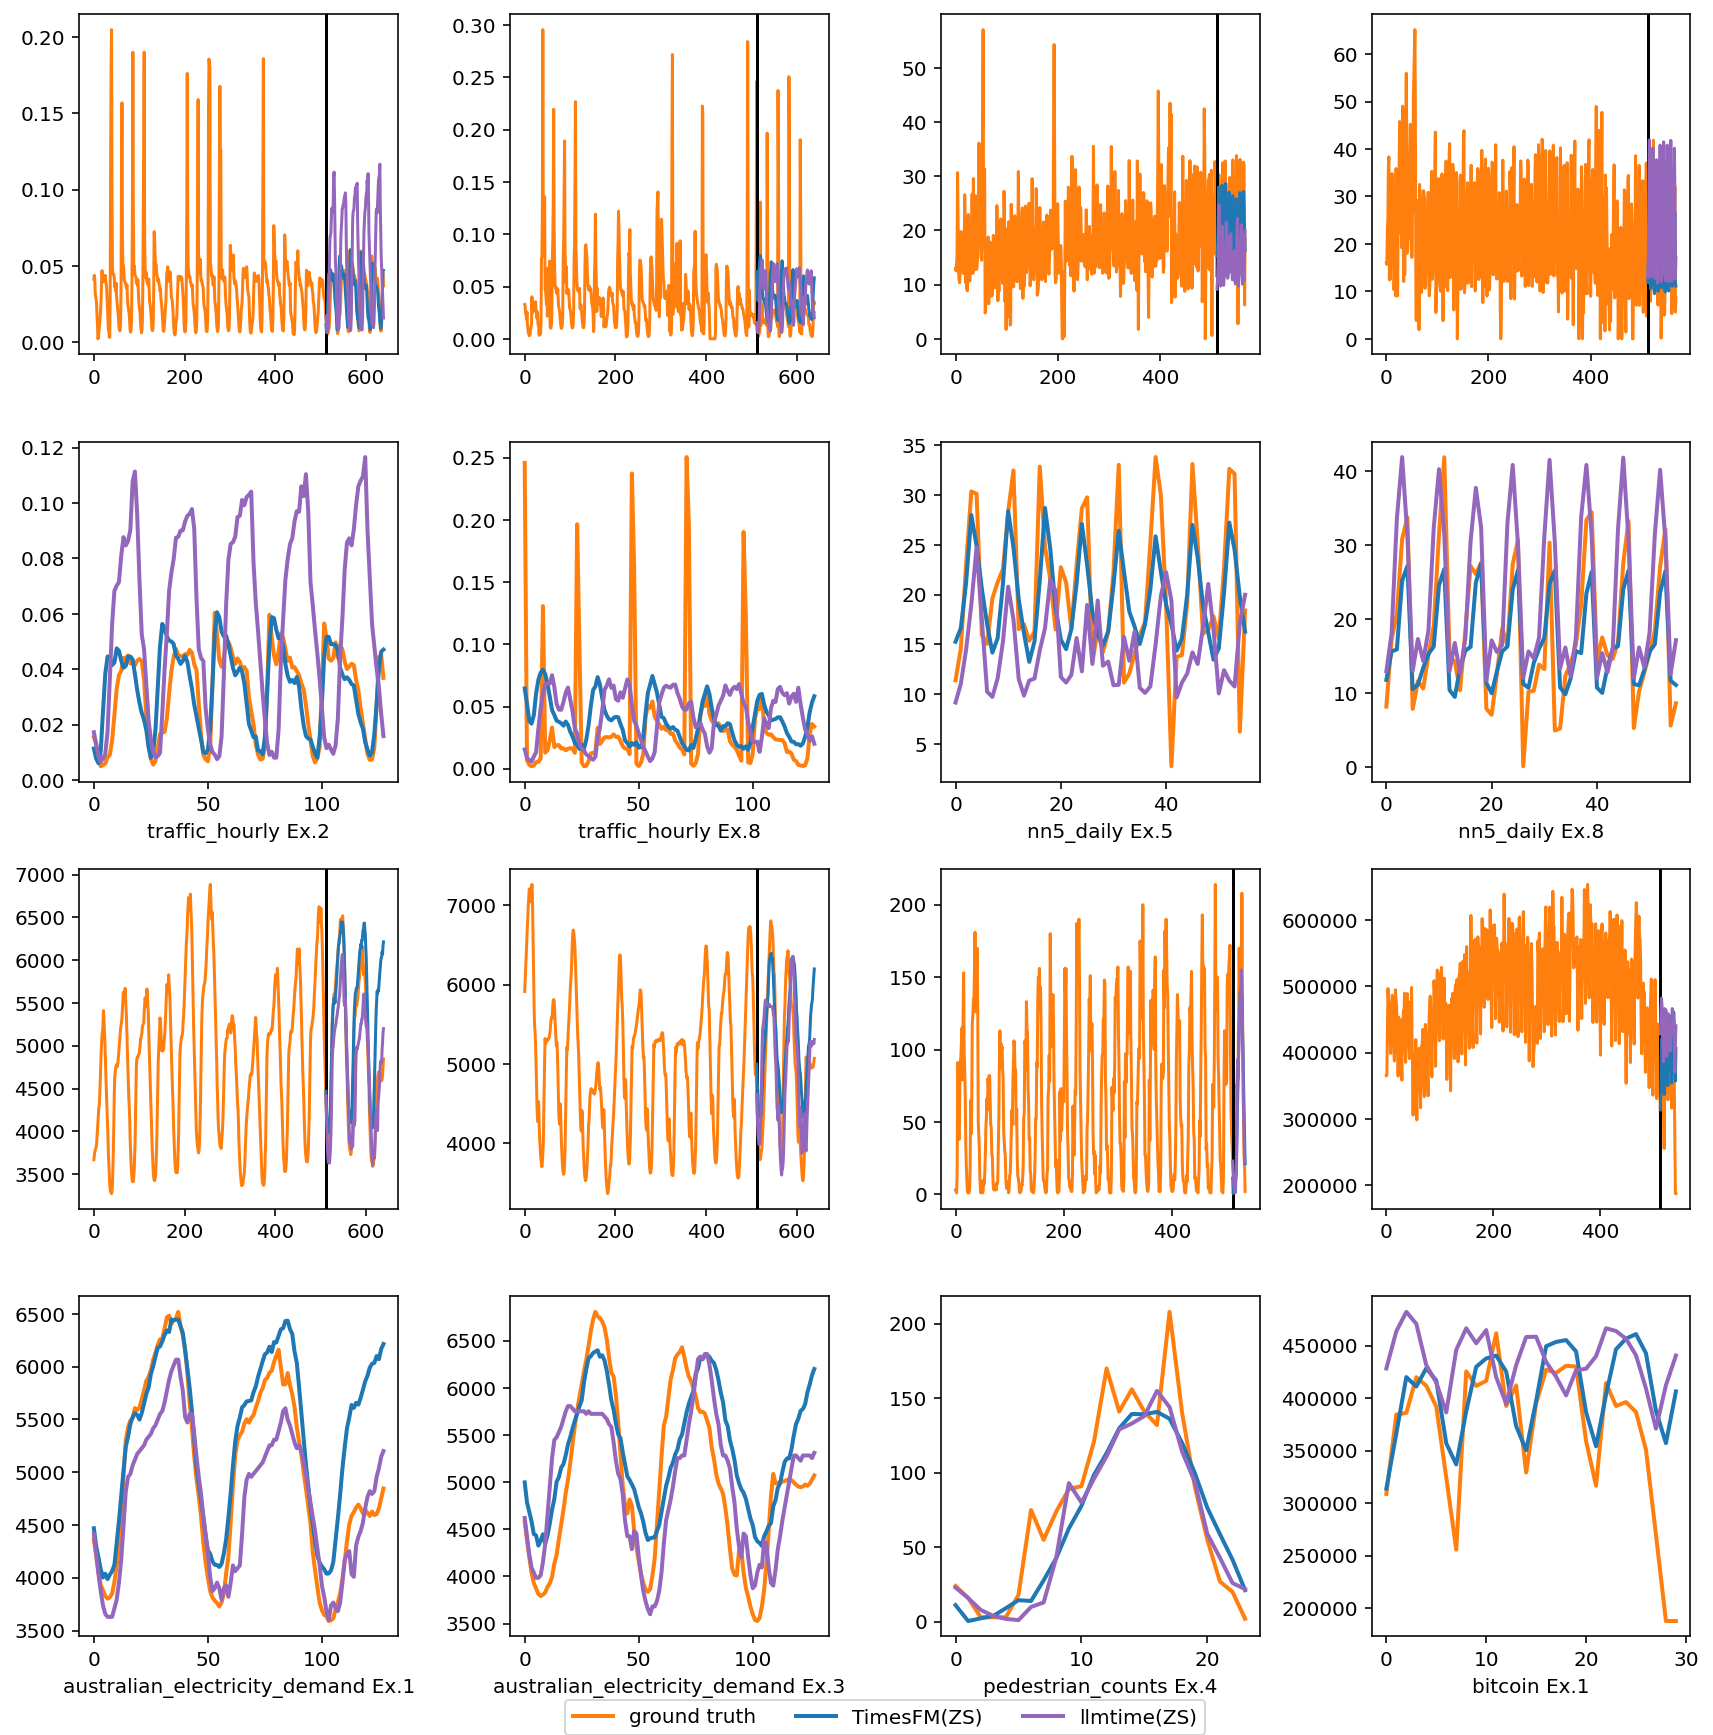
\includegraphics[width=\linewidth]{monash_4x4.png}
\caption{몇 가지 Monash 데이터 세트에서 시각화된 예측. 두 번째 행은 명확성을 위해 예측 범위를 확대하여 표시합니다.}
\label{fig:monash_4x4}
\end{figure}


% \subsubsection{Synthetic Data Visualizations}


% In this section we aim to investigate how \ours~generalizes to some common temporal patterns that are potentially out of distribution from the synthetic parts of its pretraining dataset. We present some examples in Figure~\ref{fig:syn_4x4}. We also compare how ARIMA and llmtime behaves on these examples.

% In particular, we generate these curves by (i) and (ii) linear trend + ARMA(2, 1), (iii) sum of 5 sines of different periods, (iv) and (v) a sine curve scaled linearly, (vi) a sine curve with a linear trend, (vii) a sine curve capped linearly, and (viii) minimum of two sines with a linear trend.

% We notice that, compared to (Auto)ARIMA and llmtime, \ours~is more capable of following trends and nuanced seasonal patterns. For example, Plot 3 shows the sum of 5 sine curves which is out of the distribution of our synthetic dataset. However \ours~ still correctly identifies the seasonal pattern, likely because similar pattern occurred in the context. Plot 4 and 5 demonstrate that \ours~correctly identifies the multiplicative trend which seems hard for either llmtime or ARIMA.

% It is worth pointing out that \ours~is practically the fastest and the easiest forecasting method to run here. In order for (Auto)ARIMA to work the best one needs to properly identify the seasonal length and the trend. Even so the per time-series optimization takes way longer then \ours~simply decoding.




\end{document}
